%&preformat-disser
\RequirePackage[l2tabu,orthodox]{nag} % Раскомментировав, можно в логе получать рекомендации относительно правильного использования пакетов и предупреждения об устаревших и нерекомендуемых пакетах
% Формат А4, 14pt (ГОСТ Р 7.0.11-2011, 5.3.6)
\documentclass[a4paper,14pt,oneside,openany]{memoir}

%%%%%%%%%%%%%%%%%%%%%%%%%%%%%%%%%%%%%%%%%%%%%%%%%%%%%%
%%%% Файл упрощённых настроек шаблона диссертации %%%%
%%%%%%%%%%%%%%%%%%%%%%%%%%%%%%%%%%%%%%%%%%%%%%%%%%%%%%

%%% Инициализирование переменных, не трогать!  %%%
\newcounter{intvl}
\newcounter{otstup}
\newcounter{contnumeq}
\newcounter{contnumfig}
\newcounter{contnumtab}
\newcounter{pgnum}
\newcounter{chapstyle}
\newcounter{headingdelim}
\newcounter{headingalign}
\newcounter{headingsize}
\newcounter{tabcap}
\newcounter{tablaba}
\newcounter{tabtita}
%%%%%%%%%%%%%%%%%%%%%%%%%%%%%%%%%%%%%%%%%%%%%%%%%%%%%%

%%% Область упрощённого управления оформлением %%%

%% Интервал между заголовками и между заголовком и текстом %%
% Заголовки отделяют от текста сверху и снизу
% тремя интервалами (ГОСТ Р 7.0.11-2011, 5.3.5)
\setcounter{intvl}{3}               % Коэффициент кратности к размеру шрифта

%% Отступы у заголовков в тексте %%
\setcounter{otstup}{0}              % 0 --- без отступа; 1 --- абзацный отступ

%% Нумерация формул, таблиц и рисунков %%
% Нумерация формул
\setcounter{contnumeq}{0}   % 0 --- пораздельно (во введении подряд,
                            %       без номера раздела);
                            % 1 --- сквозная нумерация по всей диссертации
% Нумерация рисунков
\setcounter{contnumfig}{0}  % 0 --- пораздельно (во введении подряд,
                            %       без номера раздела);
                            % 1 --- сквозная нумерация по всей диссертации
% Нумерация таблиц
\setcounter{contnumtab}{0}  % 0 --- пораздельно (во введении подряд,
                            %       без номера раздела);
                            % 1 --- сквозная нумерация по всей диссертации

%% Оглавление %%
\setcounter{pgnum}{1}       % 0 --- номера страниц никак не обозначены;
                            % 1 --- Стр. над номерами страниц (дважды
                            %       компилировать после изменения настройки)
\settocdepth{subsection}    % до какого уровня подразделов выносить в оглавление
\setsecnumdepth{subsection} % до какого уровня нумеровать подразделы


%% Текст и форматирование заголовков %%
\setcounter{chapstyle}{1}     % 0 --- разделы только под номером;
                              % 1 --- разделы с названием "Глава" перед номером
\setcounter{headingdelim}{1}  % 0 --- номер отделен пропуском в 1em или \quad;
                              % 1 --- номера разделов и приложений отделены
                              %       точкой с пробелом, подразделы пропуском
                              %       без точки;
                              % 2 --- номера разделов, подразделов и приложений
                              %       отделены точкой с пробелом.

%% Выравнивание заголовков в тексте %%
\setcounter{headingalign}{0}  % 0 --- по центру;
                              % 1 --- по левому краю

%% Размеры заголовков в тексте %%
\setcounter{headingsize}{0}   % 0 --- по ГОСТ, все всегда 14 пт;
                              % 1 --- пропорционально изменяющийся размер
                              %       в зависимости от базового шрифта

%% Подпись таблиц %%
\setcounter{tabcap}{0}  % 0 --- по ГОСТ, номер таблицы и название разделены
                        %       тире, выровнены по левому краю, при
                        %       необходимостина нескольких строках;
                        % 1 --- подпись таблицы не по ГОСТ, на двух и более
                        %       строках, дальнейшие настройки:
%Выравнивание первой строки, с подписью и номером
\setcounter{tablaba}{2} % 0 --- по левому краю;
                        % 1 --- по центру;
                        % 2 --- по правому краю
%Выравнивание строк с самим названием таблицы
\setcounter{tabtita}{1} % 0 --- по левому краю;
                        % 1 --- по центру;
                        % 2 --- по правому краю
%Разделитель записи «Таблица #» и названия таблицы
\newcommand{\tablabelsep}{ }

%% Подпись рисунков %%
%Разделитель записи «Рисунок #» и названия рисунка
\newcommand{\figlabelsep}{~\cyrdash\ }  % (ГОСТ 2.105, 4.3.1)
                                        % "--- здесь не работает

%%% Цвета гиперссылок %%%
% Latex color definitions: http://latexcolor.com/
\definecolor{linkcolor}{rgb}{0.9,0,0}
\definecolor{citecolor}{rgb}{0,0.6,0}
\definecolor{urlcolor}{rgb}{0,0,1}
%\definecolor{linkcolor}{rgb}{0,0,0} %black
%\definecolor{citecolor}{rgb}{0,0,0} %black
%\definecolor{urlcolor}{rgb}{0,0,0} %black
            % общие настройки шаблона
%%% Проверка используемого TeX-движка %%%
\newif\ifxetexorluatex   % определяем новый условный оператор (http://tex.stackexchange.com/a/47579)
\ifxetex
    \xetexorluatextrue
\else
    \ifluatex
        \xetexorluatextrue
    \else
        \xetexorluatexfalse
    \fi
\fi

\newif\ifsynopsis           % Условие, проверяющее, что документ --- автореферат

\usepackage{etoolbox}[2015/08/02]               % Для продвинутой проверки разных условий
\providebool{presentation}

%%% Поля и разметка страницы %%%
\usepackage{pdflscape}                              % Для включения альбомных страниц
\usepackage{geometry}                               % Для последующего задания полей
\usepackage{changepage}

%\usepackage{caption}                               % Для подписей

%%% Математические пакеты %%%
\usepackage{amsthm,amsmath,amscd}   % Математические дополнения от AMS
\usepackage{amsfonts,amssymb}       % Математические дополнения от AMS
\usepackage{mathtools}              % Добавляет окружение multlined
\usepackage{xfrac}                  % Красивые дроби
\usepackage[
    locale = DE,
    list-separator       = {;\,},
    list-final-separator = {;\,},
    list-pair-separator  = {;\,},
    range-phrase={\text{\ensuremath{-}}},
    % quotient-mode        = fraction, % красивые дроби могут не соответствовать ГОСТ
    fraction-function    = \sfrac,
    separate-uncertainty,
    ]{siunitx}                      % Размерности SI
\sisetup{inter-unit-product = \ensuremath{{}\cdot{}}}

% Кириллица в нумерации subequations
% Для правильной работы требуется выполнение сразу после загрузки пакетов
\patchcmd{\subequations}{\def\theequation{\theparentequation\alph{equation}}}
{\def\theequation{\theparentequation\asbuk{equation}}}
{\typeout{subequations patched}}{\typeout{subequations not patched}}

%%%% Установки для размера шрифта 14 pt %%%%
%% Формирование переменных и констант для сравнения (один раз для всех подключаемых файлов)%%
%% должно располагаться до вызова пакета fontspec или polyglossia, потому что они сбивают его работу
\newlength{\curtextsize}
\newlength{\bigtextsize}
\setlength{\bigtextsize}{13.9pt}

\makeatletter
%\show\f@size                                       % неплохо для отслеживания, но вызывает стопорение процесса, если документ компилируется без команды  -interaction=nonstopmode
\setlength{\curtextsize}{\f@size pt}
\makeatother

%%% Кодировки и шрифты %%%
\ifxetexorluatex
    \PassOptionsToPackage{no-math}{fontspec}        % https://tex.stackexchange.com/a/26295/104425
    \usepackage{polyglossia}[2014/05/21]            % Поддержка многоязычности (fontspec подгружается автоматически)
\else
   %%% Решение проблемы копирования текста в буфер кракозябрами
    \ifnumequal{\value{usealtfont}}{0}{}{
        \input glyphtounicode.tex
        \input glyphtounicode-cmr.tex %from pdfx package
        \pdfgentounicode=1
    }
    \usepackage{cmap}                               % Улучшенный поиск русских слов в полученном pdf-файле
    \ifnumequal{\value{usealtfont}}{2}{}{
        \defaulthyphenchar=127                      % Если стоит до fontenc, то переносы не впишутся в выделяемый текст при копировании его в буфер обмена
    }
    \usepackage{textcomp}
    \usepackage[T1,T2A]{fontenc}                    % Поддержка русских букв
    \ifnumequal{\value{usealtfont}}{1}{% Используется pscyr, при наличии
        \IfFileExists{pscyr.sty}{\usepackage{pscyr}}{}  % Подключение pscyr
    }{}
    \usepackage[utf8]{inputenc}[2014/04/30]         % Кодировка utf8
    \usepackage[english, russian]{babel}[2014/03/24]% Языки: русский, английский
    \ifnumequal{\value{usealtfont}}{2}{
        % http://dxdy.ru/post1238763.html#p1238763
        \usepackage[scaled=0.960]{XCharter}[2017/12/19] % Подключение русифицированных шрифтов XCharter
        \usepackage[charter, vvarbb, scaled=1.048]{newtxmath}[2017/12/14]
        \ifpresentation
        \else
            \setDisplayskipStretch{-0.078}
        \fi
    }{}
\fi

%%% Оформление абзацев %%%
\usepackage{indentfirst}                            % Красная строка

%%% Цвета %%%
\ifpresentation
\else
    \usepackage[dvipsnames, table, hyperref]{xcolor} % Совместимо с tikz
\fi

%%% Таблицы %%%
\usepackage{longtable,ltcaption} % Длинные таблицы
\usepackage{multirow,makecell}   % Улучшенное форматирование таблиц
\usepackage{tabu, tabulary}      % таблицы с автоматически подбирающейся
                                 % шириной столбцов (tabu обязательно
                                 % до hyperref вызывать)
\usepackage{threeparttable}      % автоматический подгон ширины подписи таблицы
\usepackage{diagbox}             % Диагональные клетки

%%% Общее форматирование
\usepackage{soulutf8}                               % Поддержка переносоустойчивых подчёркиваний и зачёркиваний
\usepackage{icomma}                                 % Запятая в десятичных дробях

%%% Оптимизация расстановки переносов и длины последней строки абзаца
\IfFileExists{impnattypo.sty}{% проверка установленности пакета impnattypo
    \ifluatex
        \ifnumequal{\value{draft}}{1}{% Черновик
            \usepackage[hyphenation, lastparline, nosingleletter, homeoarchy,
            rivers, draft]{impnattypo}
        }{% Чистовик
            \usepackage[hyphenation, lastparline, nosingleletter]{impnattypo}
        }
    \else
        \usepackage[hyphenation, lastparline]{impnattypo}
    \fi
}{}

%% Векторная графика

\usepackage{tikz}                   % Продвинутый пакет векторной графики
\usetikzlibrary{chains}             
\usetikzlibrary{shapes.geometric}   
\usetikzlibrary{shapes.symbols}     
\usetikzlibrary{arrows}             
\usetikzlibrary{positioning,decorations.pathreplacing}

%%% Гиперссылки %%%
\usepackage{hyperref}[2012/11/06]

%%% Изображения %%%
\usepackage{graphicx}[2014/04/25]                   % Подключаем пакет работы с графикой

%%% Счётчики %%%
\usepackage[figure,table]{totalcount}               % Счётчик рисунков и таблиц
\usepackage{totcount}                               % Пакет создания счётчиков на основе последнего номера подсчитываемого элемента (может требовать дважды компилировать документ)
\usepackage{totpages}                               % Счётчик страниц, совместимый с hyperref (ссылается на номер последней страницы). Желательно ставить последним пакетом в преамбуле

%%% Продвинутое управление групповыми ссылками (пока только формулами) %%%
\ifpresentation
\else
    \usepackage[russian]{cleveref} % cleveref имеет сложности со считыванием
    % языка из babel. Такое решение русификации вывода выбрано вместо
    % определения в documentclass из опасности что-то лишнее передать во все
    % остальные пакеты, включая библиографию.
    \creflabelformat{equation}{#2#1#3} % Формат по умолчанию ставил круглые
    % скобки вокруг каждого номера ссылки, теперь просто номера ссылок без
    % какого-либо дополнительного оформления
    \crefrangelabelformat{equation}{#3#1#4\cyrdash#5#2#6} % Интервалы в русском
    % языке принято делать через тире, если иное не оговорено

    % решение проблемы с "и" в \labelcref
    % https://tex.stackexchange.com/a/455124/104425
    \ifxetexorluatex
        \DeclareTextSymbol{\cyri}\UnicodeEncodingName{"0438} % и
    \fi

    % Добавление возможности использования пробелов в \labelcref
    % https://tex.stackexchange.com/a/340502/104425
    \usepackage{kvsetkeys}
    \makeatletter
    \let\org@@cref\@cref
    \renewcommand*{\@cref}[2]{%
        \edef\process@me{%
            \noexpand\org@@cref{#1}{\zap@space#2 \@empty}%
        }\process@me
    }
    \makeatother

    \newcommand{\eqrefs}[1]{(\labelcref{#1})}
    \newcommand{\refs}[1]{\labelcref{#1}}
\fi

\ifnumequal{\value{draft}}{1}{% Черновик
    \usepackage[firstpage]{draftwatermark}
    \SetWatermarkText{DRAFT}
    \SetWatermarkFontSize{14pt}
    \SetWatermarkScale{15}
    \SetWatermarkAngle{45}
}{}

%%% Исправление положения якорей подписей (под)рисунков %%%
% Без hypcap и патча, при клике по ссылке на подрисунок, просмотрщик pdf прыгает "к подписи" а не "к рисунку".
% Подробнее: https://github.com/AndreyAkinshin/Russian-Phd-LaTeX-Dissertation-Template/issues/238
% (!) Даже с патчем, если мешать в одной фиге разные типы подфиг (subbottom и subcaption) - ссылки всё равно будут работать неправильно  (см. https://www.overleaf.com/read/czmbmmtnqrrg ).
\ifpresentation
\else
    \usepackage[all]{hypcap}

    \makeatletter
    \ltx@ifclasslater{memoir}{2018/12/13}{
        % Предполагается, что в следующей версии класс будет исправлен
        \typeout{Assuming this version of memoir is free from the jumping-to-caption bug.}
    }{
        \usepackage{xpatch}

        \newcommand\mem@step@subcounter{\refstepcounter{sub\@captype}\@contkeep}

        \xpatchcmd{\@memsubbody}%
        {\refstepcounter{sub\@captype}\@contkeep}% search pattern
        {}% replacement
        {\typeout{@memsubbody is patched}}%
        {\typeout{@memsubbody is NOT patched}}%

        \xpatchcmd{\@memcontsubbody}%
        {\refstepcounter{sub\@captype}\@contkeep}% pattern
        {}% replacement
        {\typeout{@memcontsubbody is patched}}%
        {\typeout{@memcontsubbody is NOT patched}}%

        \xpatchcmd{\@memsubfloat}%
        {\vbox\bgroup}% search pattern
        {\vbox\bgroup\mem@step@subcounter}% replacement
        {\typeout{@memsubfloat patch is ok}}%
        {\typeout{@memsubfloat patch is NOT ok}}%

        \xpatchcmd{\subcaption}%
        {\refstepcounter{sub\@captype}}% search pattern
        {\H@refstepcounter{sub\@captype}}% replacement
        {\typeout{subcaption second patch is ok}}%
        {\typeout{subcaption second patch is NOT ok}}%
    }
    \makeatother
\fi

%%% Цитата, не приводимая в автореферате:
% возможно, актуальна только для biblatex
%\newcommand{\citeinsynopsis}[1]{\ifsynopsis\else ~\cite{#1} \fi}

% если текущий процесс запущен библиотекой tikz-external, то прекомпиляция должна быть включена
\ifdefined\tikzexternalrealjob
    \setcounter{imgprecompile}{1}
\fi

\ifnumequal{\value{imgprecompile}}{1}{% Только если у нас включена предкомпиляция
    \usetikzlibrary{external}   % подключение возможности предкомпиляции
    \tikzexternalize[prefix=images/cache/] % activate! % здесь можно указать отдельную папку для скомпилированных файлов
    \ifxetex
        \tikzset{external/up to date check={diff}}
    \fi
}{}
         % Пакеты общие для диссертации и автореферата
\synopsisfalse                      % Этот документ --- не автореферат
%%% Прикладные пакеты %%%
%\usepackage{calc}               % Пакет для расчётов параметров, например длины

%%% Для добавления Стр. над номерами страниц в оглавлении
%%% http://tex.stackexchange.com/a/306950
\usepackage{afterpage}

%%% Списки %%%
\usepackage{enumitem}

\usepackage{adjustbox}
    % Пакеты для диссертации
\usepackage{fr-longtable}    %ради \endlasthead

% Листинги с исходным кодом программ
\usepackage{fancyvrb}
\usepackage{listings}
\lccode`\~=0\relax %Без этого хака из-за особенностей пакета listings перестают работать конструкции с \MakeLowercase и т. п. в (xe|lua)latex

% Русская традиция начертания греческих букв
\usepackage{upgreek} % прямые греческие ради русской традиции

%%% Микротипографика
%\ifnumequal{\value{draft}}{0}{% Только если у нас режим чистовика
%    \usepackage[final, babel, shrink=45]{microtype}[2016/05/14] % улучшает представление букв и слов в строках, может помочь при наличии отдельно висящих слов
%}{}

% Отметка о версии черновика на каждой странице
% Чтобы работало надо в своей локальной копии по инструкции
% https://www.ctan.org/pkg/gitinfo2 создать небходимые файлы в папке
% ./git/hooks
% If you’re familiar with tweaking git, you can probably work it out for
% yourself. If not, I suggest you follow these steps:
% 1. First, you need a git repository and working tree. For this example,
% let’s suppose that the root of the working tree is in ~/compsci
% 2. Copy the file post-xxx-sample.txt (which is in the same folder of
% your TEX distribution as this pdf) into the git hooks directory in your
% working copy. In our example case, you should end up with a file called
% ~/compsci/.git/hooks/post-checkout
% 3. If you’re using a unix-like system, don’t forget to make the file executable.
% Just how you do this is outside the scope of this manual, but one
% possible way is with commands such as this:
% chmod g+x post-checkout.
% 4. Test your setup with “git checkout master” (or another suitable branch
% name). This should generate copies of gitHeadInfo.gin in the directories
% you intended.
% 5. Now make two more copies of this file in the same directory (hooks),
% calling them post-commit and post-merge, and you’re done. As before,
% users of unix-like systems should ensure these files are marked as
% executable.
\ifnumequal{\value{draft}}{1}{% Черновик
   \IfFileExists{.git/gitHeadInfo.gin}{
      \usepackage[mark,pcount]{gitinfo2}
      \renewcommand{\gitMark}{rev.\gitAbbrevHash\quad\gitCommitterEmail\quad\gitAuthorIsoDate}
      \renewcommand{\gitMarkFormat}{\rmfamily\color{Gray}\small\bfseries}
   }{}
}{}

%гостовая нумерация
\usepackage{enumitem}
   % Пакеты для специфических пользовательских задач

%%%%%%%%%%%%%%%%%%%%%%%%%%%%%%%%%%%%%%%%%%%%%%%%%%%%%%
%%%% Файл упрощённых настроек шаблона диссертации %%%%
%%%%%%%%%%%%%%%%%%%%%%%%%%%%%%%%%%%%%%%%%%%%%%%%%%%%%%

%%% Инициализирование переменных, не трогать!  %%%
\newcounter{intvl}
\newcounter{otstup}
\newcounter{contnumeq}
\newcounter{contnumfig}
\newcounter{contnumtab}
\newcounter{pgnum}
\newcounter{chapstyle}
\newcounter{headingdelim}
\newcounter{headingalign}
\newcounter{headingsize}
\newcounter{tabcap}
\newcounter{tablaba}
\newcounter{tabtita}
%%%%%%%%%%%%%%%%%%%%%%%%%%%%%%%%%%%%%%%%%%%%%%%%%%%%%%

%%% Область упрощённого управления оформлением %%%

%% Интервал между заголовками и между заголовком и текстом %%
% Заголовки отделяют от текста сверху и снизу
% тремя интервалами (ГОСТ Р 7.0.11-2011, 5.3.5)
\setcounter{intvl}{3}               % Коэффициент кратности к размеру шрифта

%% Отступы у заголовков в тексте %%
\setcounter{otstup}{0}              % 0 --- без отступа; 1 --- абзацный отступ

%% Нумерация формул, таблиц и рисунков %%
% Нумерация формул
\setcounter{contnumeq}{0}   % 0 --- пораздельно (во введении подряд,
                            %       без номера раздела);
                            % 1 --- сквозная нумерация по всей диссертации
% Нумерация рисунков
\setcounter{contnumfig}{0}  % 0 --- пораздельно (во введении подряд,
                            %       без номера раздела);
                            % 1 --- сквозная нумерация по всей диссертации
% Нумерация таблиц
\setcounter{contnumtab}{0}  % 0 --- пораздельно (во введении подряд,
                            %       без номера раздела);
                            % 1 --- сквозная нумерация по всей диссертации

%% Оглавление %%
\setcounter{pgnum}{1}       % 0 --- номера страниц никак не обозначены;
                            % 1 --- Стр. над номерами страниц (дважды
                            %       компилировать после изменения настройки)
\settocdepth{subsection}    % до какого уровня подразделов выносить в оглавление
\setsecnumdepth{subsection} % до какого уровня нумеровать подразделы


%% Текст и форматирование заголовков %%
\setcounter{chapstyle}{1}     % 0 --- разделы только под номером;
                              % 1 --- разделы с названием "Глава" перед номером
\setcounter{headingdelim}{1}  % 0 --- номер отделен пропуском в 1em или \quad;
                              % 1 --- номера разделов и приложений отделены
                              %       точкой с пробелом, подразделы пропуском
                              %       без точки;
                              % 2 --- номера разделов, подразделов и приложений
                              %       отделены точкой с пробелом.

%% Выравнивание заголовков в тексте %%
\setcounter{headingalign}{0}  % 0 --- по центру;
                              % 1 --- по левому краю

%% Размеры заголовков в тексте %%
\setcounter{headingsize}{0}   % 0 --- по ГОСТ, все всегда 14 пт;
                              % 1 --- пропорционально изменяющийся размер
                              %       в зависимости от базового шрифта

%% Подпись таблиц %%
\setcounter{tabcap}{0}  % 0 --- по ГОСТ, номер таблицы и название разделены
                        %       тире, выровнены по левому краю, при
                        %       необходимостина нескольких строках;
                        % 1 --- подпись таблицы не по ГОСТ, на двух и более
                        %       строках, дальнейшие настройки:
%Выравнивание первой строки, с подписью и номером
\setcounter{tablaba}{2} % 0 --- по левому краю;
                        % 1 --- по центру;
                        % 2 --- по правому краю
%Выравнивание строк с самим названием таблицы
\setcounter{tabtita}{1} % 0 --- по левому краю;
                        % 1 --- по центру;
                        % 2 --- по правому краю
%Разделитель записи «Таблица #» и названия таблицы
\newcommand{\tablabelsep}{ }

%% Подпись рисунков %%
%Разделитель записи «Рисунок #» и названия рисунка
\newcommand{\figlabelsep}{~\cyrdash\ }  % (ГОСТ 2.105, 4.3.1)
                                        % "--- здесь не работает

%%% Цвета гиперссылок %%%
% Latex color definitions: http://latexcolor.com/
\definecolor{linkcolor}{rgb}{0.9,0,0}
\definecolor{citecolor}{rgb}{0,0.6,0}
\definecolor{urlcolor}{rgb}{0,0,1}
%\definecolor{linkcolor}{rgb}{0,0,0} %black
%\definecolor{citecolor}{rgb}{0,0,0} %black
%\definecolor{urlcolor}{rgb}{0,0,0} %black
      % Упрощённые настройки шаблона

% Новые переменные, которые могут использоваться во всём проекте
% ГОСТ 7.0.11-2011
% 9.2 Оформление текста автореферата диссертации
% 9.2.1 Общая характеристика работы включает в себя следующие основные структурные
% элементы:
% актуальность темы исследования;
\newcommand{\actualityTXT}{Актуальность темы.}
% степень ее разработанности;
\newcommand{\progressTXT}{Степень разработанности темы.}
% цели и задачи;
\newcommand{\aimTXT}{Целью}
\newcommand{\tasksTXT}{задачи}
% научную новизну;
\newcommand{\noveltyTXT}{Научная новизна:}
% теоретическую и практическую значимость работы;
%\newcommand{\influenceTXT}{Теоретическая и практическая значимость}
% или чаще используют просто
\newcommand{\influenceTXT}{Практическая значимость}
% методологию и методы исследования;
\newcommand{\methodsTXT}{Методология и методы исследования.}
% положения, выносимые на защиту;
\newcommand{\defpositionsTXT}{Основные положения, выносимые на~защиту:}
% степень достоверности и апробацию результатов.
\newcommand{\reliabilityTXT}{Достоверность}
\newcommand{\probationTXT}{Апробация работы.}

\newcommand{\contributionTXT}{Личный вклад.}
\newcommand{\publicationsTXT}{Публикации.}


%%% Заголовки библиографии:

% для автореферата:
\newcommand{\bibtitleauthor}{Публикации автора по теме диссертации}

% для стиля библиографии `\insertbiblioauthorgrouped`
\newcommand{\bibtitleauthorvak}{В изданиях из списка ВАК РФ}
\newcommand{\bibtitleauthorscopus}{В изданиях, входящих в международную базу цитирования Scopus}
\newcommand{\bibtitleauthorwos}{В изданиях, входящих в международную базу цитирования Web of Science}
\newcommand{\bibtitleauthorother}{В прочих изданиях}
\newcommand{\bibtitleauthorconf}{В сборниках трудов конференций}

% для стиля библиографии `\insertbiblioauthorimportant`:
\newcommand{\bibtitleauthorimportant}{Наиболее значимые \protect\MakeLowercase\bibtitleauthor}

% для списка литературы в диссертации и списка чужих работ в автореферате:
\newcommand{\bibtitlefull}{Список литературы} % (ГОСТ Р 7.0.11-2011, 4)

\newcommand{\ProgModule}{ПМ АПНДВ} % Название программного модуля

\newcommand\diag[4]{%
    \multicolumn{1}{p{#2}|}{
        \hskip-\tabcolsep
        $\vcenter{
            \begin{tikzpicture}[baseline=0,anchor=south west,inner sep=#1]
                \path[use as bounding box] (0,0) rectangle (#2+2\tabcolsep,\baselineskip);
                \node[minimum width={#2+2\tabcolsep},minimum height=\baselineskip+\extrarowheight] (box) {};
                \draw (box.north west) -- (box.south east);
                \node[anchor=south west] at (box.south west) {#3};
                \node[anchor=north east] at (box.north east) {#4};
            \end{tikzpicture}
        }$\hskip-\tabcolsep
   }
}

\newcommand{\redcell}[1]{
    \cellcolor{red!30} #1 }

\newcommand{\greencell}[1]{
    \cellcolor{green!30} #1 }

\newcommand{\yellowcell}[1]{
    \cellcolor{yellow!30} #1 }

\newcommand{\rpt}[2][1]{%
    \newcounter{loopcntr}
    \forloop{loopcntr}{0}{\value{loopcntr}<#1}{#2}%
  }
         % Новые переменные, для всего проекта

%%% Основные сведения %%%
\newcommand{\thesisAuthorLastName}{\todo{Уманский}}
\newcommand{\thesisAuthorOtherNames}{\todo{Александр Александрович}}
\newcommand{\thesisAuthorInitials}{\todo{A.\,A.}}
\newcommand{\thesisAuthor}             % Диссертация, ФИО автора
{%
    \texorpdfstring{% \texorpdfstring takes two arguments and uses the first for (La)TeX and the second for pdf
        \thesisAuthorLastName~\thesisAuthorOtherNames% так будет отображаться на титульном листе или в тексте, где будет использоваться переменная
    }{%
        \thesisAuthorLastName, \thesisAuthorOtherNames% эта запись для свойств pdf-файла. В таком виде, если pdf будет обработан программами для сбора библиографических сведений, будет правильно представлена фамилия.
    }
}
\newcommand{\thesisAuthorShort}        % Диссертация, ФИО автора инициалами
{\thesisAuthorInitials~\thesisAuthorLastName}
\newcommand{\thesisUdk}                % Диссертация, УДК
{\todo{004.492.3}}
\newcommand{\thesisTitle}              % Диссертация, название
{\todo{Разработка программного модуля для анализа программ, написанных
на языке C/C++, на предмет программных закладок}}
\newcommand{\thesisSpecialtyNumber}    % Диссертация, специальность, номер
{\todo{09.03.04}}
\newcommand{\thesisSpecialtyTitle}     % Диссертация, специальность, название (название взято с сайта ВАК для примера)
{\todo{Программная инженерия}}
%% \newcommand{\thesisSpecialtyTwoNumber} % Диссертация, вторая специальность, номер
%% {\todo{XX.XX.XX}}
%% \newcommand{\thesisSpecialtyTwoTitle}  % Диссертация, вторая специальность, название
%% {\todo{Теория и~методика физического воспитания, спортивной тренировки,
%% оздоровительной и~адаптивной физической культуры}}
\newcommand{\thesisDegree}             % Диссертация, ученая степень
{\todo{студента института СПИНТЕХ}}
\newcommand{\thesisDegreeShort}        % Диссертация, ученая степень, краткая запись
{\todo{канд. физ.-мат. наук}}
\newcommand{\thesisCity}               % Диссертация, город написания диссертации
{\todo{Москва, г. Зеленоград}}
\newcommand{\thesisYear}               % Диссертация, год написания диссертации
{\todo{2020}}
\newcommand{\thesisOrganization}       % Диссертация, организация
{\todo{Федеральное государственное автономное образовательное учреждение высшего
образования <<Национальный исследовательский университет <<Московский институт электронной техники>>}}
\newcommand{\thesisOrganizationShort}  % Диссертация, краткое название организации для доклада
{\todo{НазУчДисРаб}}

\newcommand{\thesisInOrganization}     % Диссертация, организация в предложном падеже: Работа выполнена в ...
{\todo{Федеральном государственном образовательном учреждении высшего образования <<Национальный исследовательский университет
<<Московский институт электронной техники>>}}

%% \newcommand{\supervisorDead}{}           % Рисовать рамку вокруг фамилии
\newcommand{\supervisorFio}              % Научный руководитель, ФИО
{\todo{Кононова Алексадра Игоревна}}
\newcommand{\supervisorRegalia}          % Научный руководитель, регалии
{\todo{кандидат технических наук, доцент}}
\newcommand{\supervisorFioShort}         % Научный руководитель, ФИО
{\todo{А.\,И.~Кононова}}
\newcommand{\supervisorRegaliaShort}     % Научный руководитель, регалии
{\todo{уч.~ст.,~уч.~зв.}}

%% \newcommand{\supervisorTwoDead}{}        % Рисовать рамку вокруг фамилии
%% \newcommand{\supervisorTwoFio}           % Второй научный руководитель, ФИО
%% {\todo{Фамилия Имя Отчество}}
%% \newcommand{\supervisorTwoRegalia}       % Второй научный руководитель, регалии
%% {\todo{уч. степень, уч. звание}}
%% \newcommand{\supervisorTwoFioShort}      % Второй научный руководитель, ФИО
%% {\todo{И.\,О.~Фамилия}}
%% \newcommand{\supervisorTwoRegaliaShort}  % Второй научный руководитель, регалии
%% {\todo{уч.~ст.,~уч.~зв.}}

\newcommand{\opponentOneFio}           % Оппонент 1, ФИО
{\todo{Фамилия Имя Отчество}}
\newcommand{\opponentOneRegalia}       % Оппонент 1, регалии
{\todo{доктор физико-математических наук, профессор}}
\newcommand{\opponentOneJobPlace}      % Оппонент 1, место работы
{\todo{Не очень длинное название для места работы}}
\newcommand{\opponentOneJobPost}       % Оппонент 1, должность
{\todo{старший научный сотрудник}}

\newcommand{\opponentTwoFio}           % Оппонент 2, ФИО
{\todo{Фамилия Имя Отчество}}
\newcommand{\opponentTwoRegalia}       % Оппонент 2, регалии
{\todo{кандидат физико-математических наук}}
\newcommand{\opponentTwoJobPlace}      % Оппонент 2, место работы
{\todo{Основное место работы c длинным длинным длинным длинным названием}}
\newcommand{\opponentTwoJobPost}       % Оппонент 2, должность
{\todo{старший научный сотрудник}}

%% \newcommand{\opponentThreeFio}         % Оппонент 3, ФИО
%% {\todo{Фамилия Имя Отчество}}
%% \newcommand{\opponentThreeRegalia}     % Оппонент 3, регалии
%% {\todo{кандидат физико-математических наук}}
%% \newcommand{\opponentThreeJobPlace}    % Оппонент 3, место работы
%% {\todo{Основное место работы c длинным длинным длинным длинным названием}}
%% \newcommand{\opponentThreeJobPost}     % Оппонент 3, должность
%% {\todo{старший научный сотрудник}}

\newcommand{\leadingOrganizationTitle} % Ведущая организация, дополнительные строки. Удалить, чтобы не отображать в автореферате
{\todo{Федеральное государственное бюджетное образовательное учреждение высшего
профессионального образования с~длинным длинным длинным длинным названием}}

\newcommand{\defenseDate}              % Защита, дата
{\todo{DD mmmmmmmm YYYY~г.~в~XX часов}}
\newcommand{\defenseCouncilNumber}     % Защита, номер диссертационного совета
{\todo{Д\,123.456.78}}
\newcommand{\defenseCouncilTitle}      % Защита, учреждение диссертационного совета
{\todo{Название учреждения}}
\newcommand{\defenseCouncilAddress}    % Защита, адрес учреждение диссертационного совета
{\todo{Адрес}}
\newcommand{\defenseCouncilPhone}      % Телефон для справок
{\todo{+7~(0000)~00-00-00}}

\newcommand{\defenseSecretaryFio}      % Секретарь диссертационного совета, ФИО
{\todo{Фамилия Имя Отчество}}
\newcommand{\defenseSecretaryRegalia}  % Секретарь диссертационного совета, регалии
{\todo{д-р~физ.-мат. наук}}            % Для сокращений есть ГОСТы, например: ГОСТ Р 7.0.12-2011 + http://base.garant.ru/179724/#block_30000

\newcommand{\synopsisLibrary}          % Автореферат, название библиотеки
{\todo{Название библиотеки}}
\newcommand{\synopsisDate}             % Автореферат, дата рассылки
{\todo{DD mmmmmmmm YYYY года}}

% To avoid conflict with beamer class use \providecommand
\providecommand{\keywords}%            % Ключевые слова для метаданных PDF диссертации и автореферата
{}
             % Основные сведения
%%% Кодировки и шрифты %%%
\ifxetexorluatex
    \setmainlanguage[babelshorthands=true]{russian}    % Язык по-умолчанию русский с поддержкой приятных команд пакета babel
    \setotherlanguage{english}                         % Дополнительный язык = английский (в американской вариации по-умолчанию)

    % Проверка существования шрифтов. Недоступна в pdflatex
    \ifnumequal{\value{fontfamily}}{1}{
        \IfFontExistsTF{Times New Roman}{}{\setcounter{fontfamily}{0}}
    }{}
    \ifnumequal{\value{fontfamily}}{2}{
        \IfFontExistsTF{LiberationSerif}{}{\setcounter{fontfamily}{0}}
    }{}

    \ifnumequal{\value{fontfamily}}{0}{                    % Семейство шрифтов CMU. Используется как fallback
        \setmonofont{CMU Typewriter Text}                  % моноширинный шрифт
        \newfontfamily\cyrillicfonttt{CMU Typewriter Text} % моноширинный шрифт для кириллицы
        \defaultfontfeatures{Ligatures=TeX}                % стандартные лигатуры TeX, замены нескольких дефисов на тире и т. п. Настройки моноширинного шрифта должны идти до этой строки, чтобы при врезках кода программ в коде не применялись лигатуры и замены дефисов
        \setmainfont{CMU Serif}                            % Шрифт с засечками
        \newfontfamily\cyrillicfont{CMU Serif}             % Шрифт с засечками для кириллицы
        \setsansfont{CMU Sans Serif}                       % Шрифт без засечек
        \newfontfamily\cyrillicfontsf{CMU Sans Serif}      % Шрифт без засечек для кириллицы
    }

    \ifnumequal{\value{fontfamily}}{1}{                    % Семейство MS шрифтов
        \setmonofont{Courier New}                          % моноширинный шрифт
        \newfontfamily\cyrillicfonttt{Courier New}         % моноширинный шрифт для кириллицы
        \defaultfontfeatures{Ligatures=TeX}                % стандартные лигатуры TeX, замены нескольких дефисов на тире и т. п. Настройки моноширинного шрифта должны идти до этой строки, чтобы при врезках кода программ в коде не применялись лигатуры и замены дефисов
        \setmainfont{Times New Roman}                      % Шрифт с засечками
        \newfontfamily\cyrillicfont{Times New Roman}       % Шрифт с засечками для кириллицы
        \setsansfont{Arial}                                % Шрифт без засечек
        \newfontfamily\cyrillicfontsf{Arial}               % Шрифт без засечек для кириллицы
    }

    \ifnumequal{\value{fontfamily}}{2}{                    % Семейство шрифтов Liberation (https://pagure.io/liberation-fonts)
        \setmonofont{LiberationMono}[Scale=0.87] % моноширинный шрифт
        \newfontfamily\cyrillicfonttt{LiberationMono}[     % моноширинный шрифт для кириллицы
            Scale=0.87]
        \defaultfontfeatures{Ligatures=TeX}                % стандартные лигатуры TeX, замены нескольких дефисов на тире и т. п. Настройки моноширинного шрифта должны идти до этой строки, чтобы при врезках кода программ в коде не применялись лигатуры и замены дефисов
        \setmainfont{LiberationSerif}                      % Шрифт с засечками
        \newfontfamily\cyrillicfont{LiberationSerif}       % Шрифт с засечками для кириллицы
        \setsansfont{LiberationSans}                       % Шрифт без засечек
        \newfontfamily\cyrillicfontsf{LiberationSans}      % Шрифт без засечек для кириллицы
    }

\else
    \ifnumequal{\value{usealtfont}}{1}{% Используется pscyr, при наличии
        %\IfFileExists{pscyr.sty}
        {\renewcommand{\rmdefault}{ftm}}{}
    }{}
\fi
            % Определение шрифтов (частичное)
%%% Шаблон %%%
\DeclareRobustCommand{\todo}{\textcolor{black}}       % решаем проблему превращения названия цвета в результате \MakeUppercase, http://tex.stackexchange.com/a/187930, \DeclareRobustCommand protects \todo from expanding inside \MakeUppercase
\AtBeginDocument{%
    \setlength{\parindent}{2.5em}                   % Абзацный отступ. Должен быть одинаковым по всему тексту и равен пяти знакам (ГОСТ Р 7.0.11-2011, 5.3.7).
}

%%% Подписи %%%
\setlength{\abovecaptionskip}{0pt}   % Отбивка над подписью
\setlength{\belowcaptionskip}{0pt}   % Отбивка под подписью
\captionwidth{\linewidth}
\normalcaptionwidth

%%% Таблицы %%%
\ifnumequal{\value{tabcap}}{0}{%
    \newcommand{\tabcapalign}{\raggedright}  % по левому краю страницы или аналога parbox
    \renewcommand{\tablabelsep}{~\cyrdash\ } % тире как разделитель идентификатора с номером от наименования
    \newcommand{\tabtitalign}{}
}{%
    \ifnumequal{\value{tablaba}}{0}{%
        \newcommand{\tabcapalign}{\raggedright}  % по левому краю страницы или аналога parbox
    }{}

    \ifnumequal{\value{tablaba}}{1}{%
        \newcommand{\tabcapalign}{\centering}    % по центру страницы или аналога parbox
    }{}

    \ifnumequal{\value{tablaba}}{2}{%
        \newcommand{\tabcapalign}{\raggedleft}   % по правому краю страницы или аналога parbox
    }{}

    \ifnumequal{\value{tabtita}}{0}{%
        \newcommand{\tabtitalign}{\par\raggedright}  % по левому краю страницы или аналога parbox
    }{}

    \ifnumequal{\value{tabtita}}{1}{%
        \newcommand{\tabtitalign}{\par\centering}    % по центру страницы или аналога parbox
    }{}

    \ifnumequal{\value{tabtita}}{2}{%
        \newcommand{\tabtitalign}{\par\raggedleft}   % по правому краю страницы или аналога parbox
    }{}
}

\precaption{\tabcapalign} % всегда идет перед подписью или \legend
\captionnamefont{\normalfont\normalsize} % Шрифт надписи «Таблица #»; также определяет шрифт у \legend
\captiondelim{\tablabelsep} % разделитель идентификатора с номером от наименования
\captionstyle[\tabtitalign]{\tabtitalign}
\captiontitlefont{\normalfont\normalsize} % Шрифт с текстом подписи

%%% Рисунки %%%
\setfloatadjustment{figure}{%
    \setlength{\abovecaptionskip}{0pt}   % Отбивка над подписью
    \setlength{\belowcaptionskip}{0pt}   % Отбивка под подписью
    \precaption{} % всегда идет перед подписью или \legend
    \captionnamefont{\normalfont\normalsize} % Шрифт надписи «Рисунок #»; также определяет шрифт у \legend
    \captiondelim{\figlabelsep} % разделитель идентификатора с номером от наименования
    \captionstyle[\centering]{\centering} % Центрирование подписей, заданных командой \caption и \legend
    \captiontitlefont{\normalfont\normalsize} % Шрифт с текстом подписи
    \postcaption{} % всегда идет после подписи или \legend, и с новой строки
}

%%% Подписи подрисунков %%%
\newsubfloat{figure} % Включает возможность использовать подрисунки у окружений figure
\renewcommand{\thesubfigure}{\asbuk{subfigure}}           % Буквенные номера подрисунков
\subcaptionsize{\normalsize} % Шрифт подписи названий подрисунков (не отличается от основного)
\subcaptionlabelfont{\normalfont}
\subcaptionfont{\!\!) \normalfont} % Вот так тут добавили скобку после буквы.
\subcaptionstyle{\centering}
%\subcaptionsize{\fontsize{12pt}{13pt}\selectfont} % объявляем шрифт 12pt для использования в подписях, тут же надо интерлиньяж объявлять, если не наследуется

%%% Настройки гиперссылок %%%
\ifluatex
    \hypersetup{
        unicode,                % Unicode encoded PDF strings
    }
\fi

\hypersetup{
    linktocpage=true,           % ссылки с номера страницы в оглавлении, списке таблиц и списке рисунков
%    linktoc=all,                % both the section and page part are links
%    pdfpagelabels=false,        % set PDF page labels (true|false)
    plainpages=false,           % Forces page anchors to be named by the Arabic form  of the page number, rather than the formatted form
    colorlinks,                 % ссылки отображаются раскрашенным текстом, а не раскрашенным прямоугольником, вокруг текста
    linkcolor={black}, %{linkcolor},      % цвет ссылок типа ref, eqref и подобных
    citecolor={black}, %{citecolor},      % цвет ссылок-цитат
    urlcolor={black}, %{urlcolor},        % цвет гиперссылок
%    hidelinks,                  % Hide links (removing color and border)
    pdftitle={\thesisTitle},    % Заголовок
    pdfauthor={\thesisAuthor},  % Автор
    pdfsubject={\thesisSpecialtyNumber\ \thesisSpecialtyTitle},      % Тема
%    pdfcreator={Создатель},     % Создатель, Приложение
%    pdfproducer={Производитель},% Производитель, Производитель PDF
    pdfkeywords={\keywords},    % Ключевые слова
    pdflang={ru},
}
\ifnumequal{\value{draft}}{1}{% Черновик
    \hypersetup{
        draft,
    }
}{}

%%% Списки %%%
% Используем короткое тире (endash) для ненумерованных списков (ГОСТ 2.105-95, пункт 4.1.7, требует дефиса, но так лучше смотрится)
\renewcommand{\labelitemi}{\normalfont\bfseries{--}}

% Перечисление строчными буквами латинского алфавита (ГОСТ 2.105-95, 4.1.7)
%\renewcommand{\theenumi}{\alph{enumi}}
%\renewcommand{\labelenumi}{\theenumi)}

% Перечисление строчными буквами русского алфавита (ГОСТ 2.105-95, 4.1.7)
\makeatletter
\AddEnumerateCounter{\asbuk}{\russian@alph}{щ}      % Управляем списками/перечислениями через пакет enumitem, а он 'не знает' про asbuk, потому 'учим' его
\makeatother
%\renewcommand{\theenumi}{\asbuk{enumi}} %первый уровень нумерации
%\renewcommand{\labelenumi}{\theenumi)} %первый уровень нумерации
\renewcommand{\theenumii}{\asbuk{enumii}} %второй уровень нумерации
\renewcommand{\labelenumii}{\theenumii)} %второй уровень нумерации
\renewcommand{\theenumiii}{\arabic{enumiii}} %третий уровень нумерации
\renewcommand{\labelenumiii}{\theenumiii)} %третий уровень нумерации

\setlist{nosep,%                                    % Единый стиль для всех списков (пакет enumitem), без дополнительных интервалов.
    labelindent=\parindent,leftmargin=*%            % Каждый пункт, подпункт и перечисление записывают с абзацного отступа (ГОСТ 2.105-95, 4.1.8)
}

%%% Правильная нумерация приложений, рисунков и формул %%%
%% По ГОСТ 2.105, п. 4.3.8 Приложения обозначают заглавными буквами русского алфавита,
%% начиная с А, за исключением букв Ё, З, Й, О, Ч, Ь, Ы, Ъ.
%% Здесь также переделаны все нумерации русскими буквами.
\ifxetexorluatex
    \makeatletter
    \def\russian@Alph#1{\ifcase#1\or
       А\or Б\or В\or Г\or Д\or Е\or Ж\or
       И\or К\or Л\or М\or Н\or
       П\or Р\or С\or Т\or У\or Ф\or Х\or
       Ц\or Ш\or Щ\or Э\or Ю\or Я\else\xpg@ill@value{#1}{russian@Alph}\fi}
    \def\russian@alph#1{\ifcase#1\or
       а\or б\or в\or г\or д\or е\or ж\or
       и\or к\or л\or м\or н\or
       п\or р\or с\or т\or у\or ф\or х\or
       ц\or ш\or щ\or э\or ю\or я\else\xpg@ill@value{#1}{russian@alph}\fi}
    \def\cyr@Alph#1{\ifcase#1\or
        А\or Б\or В\or Г\or Д\or Е\or Ж\or
        И\or К\or Л\or М\or Н\or
        П\or Р\or С\or Т\or У\or Ф\or Х\or
        Ц\or Ш\or Щ\or Э\or Ю\or Я\else\xpg@ill@value{#1}{cyr@Alph}\fi}
    \def\cyr@alph#1{\ifcase#1\or
        а\or б\or в\or г\or д\or е\or ж\or
        и\or к\or л\or м\or н\or
        п\or р\or с\or т\or у\or ф\or х\or
        ц\or ш\or щ\or э\or ю\or я\else\xpg@ill@value{#1}{cyr@alph}\fi}
    \makeatother
\else
    \makeatletter
    \if@uni@ode
      \def\russian@Alph#1{\ifcase#1\or
        А\or Б\or В\or Г\or Д\or Е\or Ж\or
        И\or К\or Л\or М\or Н\or
        П\or Р\or С\or Т\or У\or Ф\or Х\or
        Ц\or Ш\or Щ\or Э\or Ю\or Я\else\@ctrerr\fi}
    \else
      \def\russian@Alph#1{\ifcase#1\or
        \CYRA\or\CYRB\or\CYRV\or\CYRG\or\CYRD\or\CYRE\or\CYRZH\or
        \CYRI\or\CYRK\or\CYRL\or\CYRM\or\CYRN\or
        \CYRP\or\CYRR\or\CYRS\or\CYRT\or\CYRU\or\CYRF\or\CYRH\or
        \CYRC\or\CYRSH\or\CYRSHCH\or\CYREREV\or\CYRYU\or
        \CYRYA\else\@ctrerr\fi}
    \fi
    \if@uni@ode
      \def\russian@alph#1{\ifcase#1\or
        а\or б\or в\or г\or д\or е\or ж\or
        и\or к\or л\or м\or н\or
        п\or р\or с\or т\or у\or ф\or х\or
        ц\or ш\or щ\or э\or ю\or я\else\@ctrerr\fi}
    \else
      \def\russian@alph#1{\ifcase#1\or
        \cyra\or\cyrb\or\cyrv\or\cyrg\or\cyrd\or\cyre\or\cyrzh\or
        \cyri\or\cyrk\or\cyrl\or\cyrm\or\cyrn\or
        \cyrp\or\cyrr\or\cyrs\or\cyrt\or\cyru\or\cyrf\or\cyrh\or
        \cyrc\or\cyrsh\or\cyrshch\or\cyrerev\or\cyryu\or
        \cyrya\else\@ctrerr\fi}
    \fi
    \makeatother
\fi
           % Стили общие для диссертации и автореферата
%%% Переопределение именований, если иначе не сработает %%%
\gappto\captionsrussian{
    \renewcommand{\chaptername}{Глава}
%    \renewcommand{\appendixname}{Приложение} % (ГОСТ Р 7.0.11-2011, 5.7)
}

%%% Изображения %%%
\graphicspath{{images/}{Dissertation/images/}}         % Пути к изображениям

%%% Интервалы %%%
%% По ГОСТ Р 7.0.11-2011, пункту 5.3.6 требуется полуторный интервал
%% Реализация средствами класса (на основе setspace) ближе к типографской классике.
%% И правит сразу и в таблицах (если со звёздочкой)
%\DoubleSpacing*     % Двойной интервал
\OnehalfSpacing*    % Полуторный интервал
%\setSpacing{1.42}   % Полуторный интервал, подобный Ворду (возможно, стоит включать вместе с предыдущей строкой)

%%% Макет страницы %%%
% Выставляем значения полей (ГОСТ 7.0.11-2011, 5.3.7)
%\geometry{a4paper, top=2cm, bottom=2cm, left=2.5cm, right=1cm, nofoot, nomarginpar} %, heightrounded, showframe
\geometry{a4paper, top=2cm, bottom=2cm, left=2cm, right=1cm, nofoot, nomarginpar} %, heightrounded, showframe
\setlength{\topskip}{0pt}   %размер дополнительного верхнего поля
\setlength{\footskip}{12.3pt} % снимет warning, согласно https://tex.stackexchange.com/a/334346

%%% Выравнивание и переносы %%%
%% http://tex.stackexchange.com/questions/241343/what-is-the-meaning-of-fussy-sloppy-emergencystretch-tolerance-hbadness
%% http://www.latex-community.org/forum/viewtopic.php?p=70342#p70342
\tolerance 1414
\hbadness 1414
\emergencystretch 1.5em % В случае проблем регулировать в первую очередь
\hfuzz 0.3pt
\vfuzz \hfuzz
%\raggedbottom
%\sloppy                 % Избавляемся от переполнений
\clubpenalty=10000      % Запрещаем разрыв страницы после первой строки абзаца
\widowpenalty=10000     % Запрещаем разрыв страницы после последней строки абзаца
\brokenpenalty=4991     % Ограничение на разрыв страницы, если строка заканчивается переносом

%%% Блок управления параметрами для выравнивания заголовков в тексте %%%
\newlength{\otstuplen}
\setlength{\otstuplen}{\theotstup\parindent}
\ifnumequal{\value{headingalign}}{0}{% выравнивание заголовков в тексте
    \newcommand{\hdngalign}{\centering}                % по центру
    \newcommand{\hdngaligni}{}% по центру
    \setlength{\otstuplen}{0pt}
}{%
    \newcommand{\hdngalign}{}                 % по левому краю
    \newcommand{\hdngaligni}{\hspace{\otstuplen}}      % по левому краю
} % В обоих случаях вроде бы без переноса, как и надо (ГОСТ Р 7.0.11-2011, 5.3.5)

%%% Оглавление %%%
\renewcommand{\cftchapterdotsep}{\cftdotsep}                % отбивка точками до номера страницы начала главы/раздела

%% Переносить слова в заголовке не допускается (ГОСТ Р 7.0.11-2011, 5.3.5). Заголовки в оглавлении должны точно повторять заголовки в тексте (ГОСТ Р 7.0.11-2011, 5.2.3). Прямого указания на запрет переносов в оглавлении нет, но по той же логике невнесения искажений в смысл, лучше в оглавлении не переносить:
\setrmarg{2.55em plus1fil}                             %To have the (sectional) titles in the ToC, etc., typeset ragged right with no hyphenation
\renewcommand{\cftchapterpagefont}{\normalfont}        % нежирные номера страниц у глав в оглавлении
\renewcommand{\cftchapterleader}{\cftdotfill{\cftchapterdotsep}}% нежирные точки до номеров страниц у глав в оглавлении
%\renewcommand{\cftchapterfont}{}                       % нежирные названия глав в оглавлении

\ifnumgreater{\value{headingdelim}}{0}{%
    \renewcommand\cftchapteraftersnum{.\space}       % добавляет точку с пробелом после номера раздела в оглавлении
}{}
\ifnumgreater{\value{headingdelim}}{1}{%
    \renewcommand\cftsectionaftersnum{.\space}       % добавляет точку с пробелом после номера подраздела в оглавлении
    \renewcommand\cftsubsectionaftersnum{.\space}    % добавляет точку с пробелом после номера подподраздела в оглавлении
    \renewcommand\cftsubsubsectionaftersnum{.\space} % добавляет точку с пробелом после номера подподподраздела в оглавлении
    \AtBeginDocument{% без этого polyglossia сама всё переопределяет
        \setsecnumformat{\csname the#1\endcsname.\space}
    }
}{%
    \AtBeginDocument{% без этого polyglossia сама всё переопределяет
        \setsecnumformat{\csname the#1\endcsname\quad}
    }
}

\renewcommand*{\cftappendixname}{\appendixname\space} % Слово Приложение в оглавлении

%%% Колонтитулы %%%
% Порядковый номер страницы печатают на середине верхнего поля страницы (ГОСТ Р 7.0.11-2011, 5.3.8)
\makeevenhead{plain}{}{\thepage}{}
\makeoddhead{plain}{}{\thepage}{}
\makeevenfoot{plain}{}{}{}
\makeoddfoot{plain}{}{}{}
\pagestyle{plain}

%%% добавить Стр. над номерами страниц в оглавлении
%%% http://tex.stackexchange.com/a/306950
\newif\ifendTOC

\newcommand*{\tocheader}{
\ifnumequal{\value{pgnum}}{1}{%
    \ifendTOC\else\hbox to \linewidth%
      {\noindent{}~\hfill{}}\par%
      \ifnumless{\value{page}}{3}{}{%
        \vspace{0.5\onelineskip}
      }
      \afterpage{\tocheader}
    \fi%
}{}%
}%

%%% Оформление заголовков глав, разделов, подразделов %%%
%% Работа должна быть выполнена ... размером шрифта 12-14 пунктов (ГОСТ Р 7.0.11-2011, 5.3.8). То есть не должно быть надписей шрифтом более 14. Так и поставим.
%% Эти установки будут давать одинаковый результат независимо от выбора базовым шрифтом 12 пт или 14 пт
%\newcommand{\basegostsectionfont}{\fontsize{14pt}{16pt}\selectfont\bfseries}
\newcommand{\basegostsectionfont}{\fontsize{13pt}{13pt}\selectfont\bfseries}

\makechapterstyle{thesisgost}{%
    \chapterstyle{default}
    \setlength{\beforechapskip}{0pt}
    \setlength{\midchapskip}{0pt}
    \setlength{\afterchapskip}{\theintvl\curtextsize}
    \renewcommand*{\chapnamefont}{\basegostsectionfont}
    \renewcommand*{\chapnumfont}{\basegostsectionfont}
    \renewcommand*{\chaptitlefont}{\basegostsectionfont}
    \renewcommand*{\chapterheadstart}{}
    \ifnumgreater{\value{headingdelim}}{0}{%
        \renewcommand*{\afterchapternum}{.\space}   % добавляет точку с пробелом после номера раздела
    }{%
        \renewcommand*{\afterchapternum}{\quad}     % добавляет \quad после номера раздела
    }
    \renewcommand*{\printchapternum}{\hdngaligni\hdngalign\chapnumfont \thechapter}
    \renewcommand*{\printchaptername}{}
    \renewcommand*{\printchapternonum}{\hdngaligni\hdngalign}
}

\makeatletter
\makechapterstyle{thesisgostchapname}{%
    \chapterstyle{thesisgost}
    \renewcommand*{\printchapternum}{\chapnumfont \thechapter}
    \renewcommand*{\printchaptername}{\hdngaligni\hdngalign\chapnamefont \@chapapp} %
}
\makeatother

\chapterstyle{thesisgost}

\setsecheadstyle{\basegostsectionfont\hdngalign}
\setsecindent{\otstuplen}

\setsubsecheadstyle{\basegostsectionfont\hdngalign}
\setsubsecindent{\otstuplen}

\setsubsubsecheadstyle{\basegostsectionfont\hdngalign}
\setsubsubsecindent{\otstuplen}

\sethangfrom{\noindent #1} %все заголовки подразделов центрируются с учетом номера, как block

\ifnumequal{\value{chapstyle}}{1}{%
    \chapterstyle{thesisgostchapname}
    \renewcommand*{\cftchaptername}{\chaptername\space} % будет вписано слово Глава перед каждым номером раздела в оглавлении
}{}%

%%% Интервалы между заголовками
%\setbeforesecskip{\theintvl\curtextsize}% Заголовки отделяют от текста сверху и снизу тремя интервалами (ГОСТ Р 7.0.11-2011, 5.3.5).
%\setaftersecskip{\theintvl\curtextsize}
%\setbeforesubsecskip{\theintvl\curtextsize}
%\setaftersubsecskip{\theintvl\curtextsize}
%\setbeforesubsubsecskip{\theintvl\curtextsize}
%\setaftersubsubsecskip{\theintvl\curtextsize}

%%% Вертикальные интервалы глав (\chapter) в оглавлении как и у заголовков
% раскомментировать следующие 2
% \setlength{\cftbeforechapterskip}{0pt plus 0pt}   % ИЛИ эти 2 строки из учебника
% \renewcommand*{\insertchapterspace}{}
% или эту  
% \renewcommand*{\cftbeforechapterskip}{0em}       


%%% Блок дополнительного управления размерами заголовков
\ifnumequal{\value{headingsize}}{1}{% Пропорциональные заголовки и базовый шрифт 14 пт
    \renewcommand{\basegostsectionfont}{\large\bfseries}
    \renewcommand*{\chapnamefont}{\Large\bfseries}
    \renewcommand*{\chapnumfont}{\Large\bfseries}
    \renewcommand*{\chaptitlefont}{\Large\bfseries}
}{}

%%% Счётчики %%%

%% Упрощённые настройки шаблона диссертации: нумерация формул, таблиц, рисунков
\ifnumequal{\value{contnumeq}}{1}{%
    \counterwithout{equation}{chapter} % Убираем связанность номера формулы с номером главы/раздела
}{}
\ifnumequal{\value{contnumfig}}{1}{%
    \counterwithout{figure}{chapter}   % Убираем связанность номера рисунка с номером главы/раздела
}{}
\ifnumequal{\value{contnumtab}}{1}{%
    \counterwithout{table}{chapter}    % Убираем связанность номера таблицы с номером главы/раздела
}{}


%%http://www.linux.org.ru/forum/general/6993203#comment-6994589 (используется totcount)
\makeatletter
\def\formbytotal#1#2#3#4#5{%
    \newcount\@c
    \@c\totvalue{#1}\relax
    \newcount\@last
    \newcount\@pnul
    \@last\@c\relax
    \divide\@last 10
    \@pnul\@last\relax
    \divide\@pnul 10
    \multiply\@pnul-10
    \advance\@pnul\@last
    \multiply\@last-10
    \advance\@last\@c
    \total{#1}~#2%
    \ifnum\@pnul=1#5\else%
    \ifcase\@last#5\or#3\or#4\or#4\or#4\else#5\fi
    \fi
}
\makeatother

\AtBeginDocument{
%% регистрируем счётчики в системе totcounter
    \regtotcounter{totalcount@figure}
    \regtotcounter{totalcount@table}       % Если иным способом поставить в преамбуле то ошибка в числе таблиц
    \regtotcounter{TotPages}               % Если иным способом поставить в преамбуле то ошибка в числе страниц
}
  % Стили для диссертации
\input{Dissertation/userstyles} % Стили для специфических пользовательских задач

%%% Библиография. Выбор движка для реализации %%%
% Здесь только проверка установленного ключа. Сама настройка выбора движка
% размещена в common/setup.tex
\ifnumequal{\value{bibliosel}}{0}{%
    \input{biblio/predefined}   % Встроенная реализация с загрузкой файла через движок bibtex8
}{
    %%% Реализация библиографии пакетами biblatex и biblatex-gost с использованием движка biber %%%
%\usepackage[square,comma,sort&compress,numbers]{natbib}  
\usepackage{csquotes} % biblatex рекомендует его подключать. Пакет для оформления сложных блоков цитирования.
%%% Загрузка пакета с основными настройками %%%
\makeatletter
\ifnumequal{\value{draft}}{0}{% Чистовик
\usepackage[%
backend=biber,% движок
bibencoding=utf8,% кодировка bib файла
sorting=none,% настройка сортировки списка литературы
style=gost-numeric,% стиль цитирования и библиографии (по ГОСТ)
language=autobib,% получение языка из babel/polyglossia, default: autobib % если ставить autocite или auto, то цитаты в тексте с указанием страницы, получат указание страницы на языке оригинала
autolang=other,% многоязычная библиография
clearlang=true,% внутренний сброс поля language, если он совпадает с языком из babel/polyglossia
defernumbers=true,% нумерация проставляется после двух компиляций, зато позволяет выцеплять библиографию по ключевым словам и нумеровать не из большего списка
sortcites=true,% сортировать номера затекстовых ссылок при цитировании (если в квадратных скобках несколько ссылок, то отображаться будут отсортированно, а не абы как)
doi=false,% Показывать или нет ссылки на DOI
isbn=false,% Показывать или нет ISBN, ISSN, ISRN
]{biblatex}[2016/09/17]
\ltx@iffilelater{biblatex-gost.def}{2017/05/03}%
{\toggletrue{bbx:gostbibliography}%
\renewcommand*{\revsdnamepunct}{\addcomma}}{}
}{%Черновик
\usepackage[%
backend=biber,% движок
bibencoding=utf8,% кодировка bib файла
sorting=true,% настройка сортировки списка литературы
defernumbers=true, % откомментируйте, если требуется правильная нумерация ссылок на литературу в режиме черновика. Замедляет сборку
]{biblatex}[2016/09/17]%
}
\makeatother

\ifxetexorluatex
\else
% Исправление случая неподдержки знака номера в pdflatex
    \DefineBibliographyStrings{russian}{number={\textnumero}}
\fi

\ifsynopsis
\ifnumgreater{\value{usefootcite}}{0}{
    \ExecuteBibliographyOptions{autocite=footnote}
    \newbibmacro*{cite:full}{%
        \printtext[bibhypertarget]{%
            \usedriver{%
                \DeclareNameAlias{sortname}{default}%
            }{%
                \thefield{entrytype}%
            }%
        }%
        \usebibmacro{shorthandintro}%
    }
    \DeclareCiteCommand{\smartcite}[\mkbibfootnote]{%
        \usebibmacro{prenote}%
    }{%
        \usebibmacro{citeindex}%
        \usebibmacro{cite:full}%
    }{%
        \multicitedelim%
    }{%
        \usebibmacro{postnote}%
    }
}{}
\fi

%%% Подключение файлов bib %%%
\addbibresource[label=bl-external]{biblio/external.bib}
\addbibresource[label=bl-author]{biblio/author.bib}

%http://tex.stackexchange.com/a/141831/79756
%There is a way to automatically map the language field to the langid field. The following lines in the preamble should be enough to do that.
%This command will copy the language field into the langid field and will then delete the contents of the language field. The language field will only be deleted if it was successfully copied into the langid field.
\DeclareSourcemap{ %модификация bib файла перед тем, как им займётся biblatex
    \maps{
        \map{% перекидываем значения полей language в поля langid, которыми пользуется biblatex
            \step[fieldsource=language, fieldset=langid, origfieldval, final]
            \step[fieldset=language, null]
        }
        \map{% перекидываем значения полей numpages в поля pagetotal, которыми пользуется biblatex
            \step[fieldsource=numpages, fieldset=pagetotal, origfieldval, final]
            \step[fieldset=numpages, null]
        }
        \map{% перекидываем значения полей pagestotal в поля pagetotal, которыми пользуется biblatex
            \step[fieldsource=pagestotal, fieldset=pagetotal, origfieldval, final]
            \step[fieldset=pagestotal, null]
        }
        \map[overwrite]{% перекидываем значения полей shortjournal, если они есть, в поля journal, которыми пользуется biblatex
            \step[fieldsource=shortjournal, final]
            \step[fieldset=journal, origfieldval]
            \step[fieldset=shortjournal, null]
        }
        \map[overwrite]{% перекидываем значения полей shortbooktitle, если они есть, в поля booktitle, которыми пользуется biblatex
            \step[fieldsource=shortbooktitle, final]
            \step[fieldset=booktitle, origfieldval]
            \step[fieldset=shortbooktitle, null]
        }
        \map{% если в поле medium написано "Электронный ресурс", то устанавливаем поле media, которым пользуется biblatex, в значение eresource.
            \step[fieldsource=medium,
            match=\regexp{Электронный\s+ресурс},
            final]
            \step[fieldset=media, fieldvalue=eresource]
            \step[fieldset=medium, null]
        }
        \map{% использование media=text по умолчанию
            \step[fieldset=media, fieldvalue=text]
        }
        \map[overwrite]{% стираем значения всех полей issn
            \step[fieldset=issn, null]
        }
        \map[overwrite]{% стираем значения всех полей abstract, поскольку ими не пользуемся, а там бывают "неприятные" латеху символы
            \step[fieldsource=abstract]
            \step[fieldset=abstract,null]
        }
        \map[overwrite]{ % переделка формата записи даты
            \step[fieldsource=urldate,
            match=\regexp{([0-9]{2})\.([0-9]{2})\.([0-9]{4})},
            replace={$3-$2-$1$4}, % $4 вставлен исключительно ради нормальной работы программ подсветки синтаксиса, которые некорректно обрабатывают $ в таких конструкциях
            final]
        }
        \map[overwrite]{ % стираем ключевые слова
            \step[fieldsource=keywords]
            \step[fieldset=keywords,null]
        }
        % реализация foreach различается для biblatex v3.12 и v3.13.
        % Для версии v3.13 эта конструкция заменяет последующие 5 структур map
        % \map[overwrite,foreach={authorvak,authorscopus,authorwos,authorconf,authorother}]{ % записываем информацию о типе публикации в ключевые слова
        %     \step[fieldsource=$MAPLOOP,final=true]
        %     \step[fieldset=keywords,fieldvalue={,biblio$MAPLOOP},append=true]
        % }
        \map[overwrite]{ % записываем информацию о типе публикации в ключевые слова
            \step[fieldsource=authorvak,final=true]
            \step[fieldset=keywords,fieldvalue={,biblioauthorvak},append=true]
        }
        \map[overwrite]{ % записываем информацию о типе публикации в ключевые слова
            \step[fieldsource=authorscopus,final=true]
            \step[fieldset=keywords,fieldvalue={,biblioauthorscopus},append=true]
        }
        \map[overwrite]{ % записываем информацию о типе публикации в ключевые слова
            \step[fieldsource=authorwos,final=true]
            \step[fieldset=keywords,fieldvalue={,biblioauthorwos},append=true]
        }
        \map[overwrite]{ % записываем информацию о типе публикации в ключевые слова
            \step[fieldsource=authorconf,final=true]
            \step[fieldset=keywords,fieldvalue={,biblioauthorconf},append=true]
        }
        \map[overwrite]{ % записываем информацию о типе публикации в ключевые слова
            \step[fieldsource=authorother,final=true]
            \step[fieldset=keywords,fieldvalue={,biblioauthorother},append=true]
        }
        \map[overwrite]{ % добавляем ключевые слова, чтобы различать источники
            \perdatasource{biblio/external.bib}
            \step[fieldset=keywords, fieldvalue={,biblioexternal},append=true]
        }
        \map[overwrite]{ % добавляем ключевые слова, чтобы различать источники
            \perdatasource{biblio/author.bib}
            \step[fieldset=keywords, fieldvalue={,biblioauthor},append=true]
        }
        \map[overwrite]{ % добавляем ключевые слова, чтобы различать источники
            \step[fieldset=keywords, fieldvalue={,bibliofull},append=true]
        }
%        \map[overwrite]{% стираем значения всех полей series
%            \step[fieldset=series, null]
%        }
        \map[overwrite]{% перекидываем значения полей howpublished в поля organization для типа online
            \step[typesource=online, typetarget=online, final]
            \step[fieldsource=howpublished, fieldset=organization, origfieldval]
            \step[fieldset=howpublished, null]
        }
        % Так отключаем [Электронный ресурс]
%        \map[overwrite]{% стираем значения всех полей media=eresource
%            \step[fieldsource=media,
%            match={eresource},
%            final]
%            \step[fieldset=media, null]
%        }
    }
}

\ifsynopsis
\else
\DeclareSourcemap{ %модификация bib файла перед тем, как им займётся biblatex
    \maps{
        \map[overwrite]{% стираем значения всех полей addendum
            \perdatasource{biblio/author.bib}
            \step[fieldset=addendum, null] %чтобы избавиться от информации об объёме авторских статей, в отличие от автореферата
        }
    }
}
\fi

\defbibfilter{vakscopuswos}{%
    keyword=biblioauthorvak or keyword=biblioauthorscopus or keyword=biblioauthorwos
}

\defbibfilter{scopuswos}{%
    keyword=biblioauthorscopus or keyword=biblioauthorwos
}

%%% Убираем неразрывные пробелы перед двоеточием и точкой с запятой %%%
%\makeatletter
%\ifnumequal{\value{draft}}{0}{% Чистовик
%    \renewcommand*{\addcolondelim}{%
%      \begingroup%
%      \def\abx@colon{%
%        \ifdim\lastkern>\z@\unkern\fi%
%        \abx@puncthook{:}\space}%
%      \addcolon%
%      \endgroup}
%
%    \renewcommand*{\addsemicolondelim}{%
%      \begingroup%
%      \def\abx@semicolon{%
%        \ifdim\lastkern>\z@\unkern\fi%
%        \abx@puncthook{;}\space}%
%      \addsemicolon%
%      \endgroup}
%}{}
%\makeatother

%%% Правка записей типа thesis, чтобы дважды не писался автор
%\ifnumequal{\value{draft}}{0}{% Чистовик
%\DeclareBibliographyDriver{thesis}{%
%  \usebibmacro{bibindex}%
%  \usebibmacro{begentry}%
%  \usebibmacro{heading}%
%  \newunit
%  \usebibmacro{author}%
%  \setunit*{\labelnamepunct}%
%  \usebibmacro{thesistitle}%
%  \setunit{\respdelim}%
%  %\printnames[last-first:full]{author}%Вот эту строчку нужно убрать, чтобы автор диссертации не дублировался
%  \newunit\newblock
%  \printlist[semicolondelim]{specdata}%
%  \newunit
%  \usebibmacro{institution+location+date}%
%  \newunit\newblock
%  \usebibmacro{chapter+pages}%
%  \newunit
%  \printfield{pagetotal}%
%  \newunit\newblock
%  \usebibmacro{doi+eprint+url+note}%
%  \newunit\newblock
%  \usebibmacro{addendum+pubstate}%
%  \setunit{\bibpagerefpunct}\newblock
%  \usebibmacro{pageref}%
%  \newunit\newblock
%  \usebibmacro{related:init}%
%  \usebibmacro{related}%
%  \usebibmacro{finentry}}
%}{}

%\newbibmacro{string+doi}[1]{% новая макрокоманда на простановку ссылки на doi
%    \iffieldundef{doi}{#1}{\href{http://dx.doi.org/\thefield{doi}}{#1}}}

%\ifnumequal{\value{draft}}{0}{% Чистовик
%\renewcommand*{\mkgostheading}[1]{\usebibmacro{string+doi}{#1}} % ссылка на doi с авторов. стоящих впереди записи
%\renewcommand*{\mkgostheading}[1]{#1} % только лишь убираем курсив с авторов
%}{}
%\DeclareFieldFormat{title}{\usebibmacro{string+doi}{#1}} % ссылка на doi с названия работы
%\DeclareFieldFormat{journaltitle}{\usebibmacro{string+doi}{#1}} % ссылка на doi с названия журнала
%%% Тире как разделитель в библиографии традиционной руской длины:
\renewcommand*{\newblockpunct}{\addperiod\addnbspace\cyrdash\space\bibsentence}
%%% Убрать тире из разделителей элементов в библиографии:
%\renewcommand*{\newblockpunct}{%
%    \addperiod\space\bibsentence}%block punct.,\bibsentence is for vol,etc.

%%% Возвращаем запись «Режим доступа» %%%
%\DefineBibliographyStrings{english}{%
%    urlfrom = {Mode of access}
%}
%\DeclareFieldFormat{url}{\bibstring{urlfrom}\addcolon\space\url{#1}}

%%% В списке литературы обозначение одной буквой диапазона страниц англоязычного источника %%%
\DefineBibliographyStrings{english}{%
    pages = {p\adddot} %заглавность буквы затем по месту определяется работой самого biblatex
}

%%% В ссылке на источник в основном тексте с указанием конкретной страницы обозначение одной большой буквой %%%
%\DefineBibliographyStrings{russian}{%
%    page = {C\adddot}
%}

%%% Исправление длины тире в диапазонах %%%
% \cyrdash --- тире «русской» длины, \textendash --- en-dash
\DefineBibliographyExtras{russian}{%
  \protected\def\bibrangedash{%
    \cyrdash\penalty\value{abbrvpenalty}}% almost unbreakable dash
  \protected\def\bibdaterangesep{\bibrangedash}%тире для дат
}
\DefineBibliographyExtras{english}{%
  \protected\def\bibrangedash{%
    \cyrdash\penalty\value{abbrvpenalty}}% almost unbreakable dash
  \protected\def\bibdaterangesep{\bibrangedash}%тире для дат
}

%Set higher penalty for breaking in number, dates and pages ranges
\setcounter{abbrvpenalty}{10000} % default is \hyphenpenalty which is 12

%Set higher penalty for breaking in names
\setcounter{highnamepenalty}{10000} % If you prefer the traditional BibTeX behavior (no linebreaks at highnamepenalty breakpoints), set it to ‘infinite’ (10 000 or higher).
\setcounter{lownamepenalty}{10000}

%%% Set low penalties for breaks at uppercase letters and lowercase letters
%\setcounter{biburllcpenalty}{500} %управляет разрывами ссылок после маленьких букв RTFM biburllcpenalty
%\setcounter{biburlucpenalty}{3000} %управляет разрывами ссылок после больших букв, RTFM biburlucpenalty

%%% Список литературы с красной строки (без висячего отступа) %%%
%\defbibenvironment{bibliography} % переопределяем окружение библиографии из gost-numeric.bbx пакета biblatex-gost
%  {\list
%     {\printtext[labelnumberwidth]{%
%       \printfield{prefixnumber}%
%       \printfield{labelnumber}}}
%     {%
%      \setlength{\labelwidth}{\labelnumberwidth}%
%      \setlength{\leftmargin}{0pt}% default is \labelwidth
%      \setlength{\labelsep}{\widthof{\ }}% Управляет длиной отступа после точки % default is \biblabelsep
%      \setlength{\itemsep}{\bibitemsep}% Управление дополнительным вертикальным разрывом между записями. \bibitemsep по умолчанию соответствует \itemsep списков в документе.
%      \setlength{\itemindent}{\bibhang}% Пользуемся тем, что \bibhang по умолчанию принимает значение \parindent (абзацного отступа), который переназначен в styles.tex
%      \addtolength{\itemindent}{\labelwidth}% Сдвигаем правее на величину номера с точкой
%      \addtolength{\itemindent}{\labelsep}% Сдвигаем ещё правее на отступ после точки
%      \setlength{\parsep}{\bibparsep}%
%     }%
%      \renewcommand*{\makelabel}[1]{\hss##1}%
%  }
%  {\endlist}
%  {\item}

%%% Макросы автоматического подсчёта количества авторских публикаций.
% Печатают невидимую (пустую) библиографию, считая количество источников.
% http://tex.stackexchange.com/a/66851/79756
%
\makeatletter
        \newtotcounter{citenum}
        \defbibenvironment{counter}
            {\setcounter{citenum}{0}\renewcommand{\blx@driver}[1]{}} % begin code: убирает весь выводимый текст
            {} % end code
            {\stepcounter{citenum}} % item code: cчитает "печатаемые в библиографию" источники

        \newtotcounter{citeauthorvak}
        \defbibenvironment{countauthorvak}
            {\setcounter{citeauthorvak}{0}\renewcommand{\blx@driver}[1]{}}
            {}
            {\stepcounter{citeauthorvak}}

        \newtotcounter{citeauthorscopus}
        \defbibenvironment{countauthorscopus}
                {\setcounter{citeauthorscopus}{0}\renewcommand{\blx@driver}[1]{}}
                {}
                {\stepcounter{citeauthorscopus}}

        \newtotcounter{citeauthorwos}
        \defbibenvironment{countauthorwos}
                {\setcounter{citeauthorwos}{0}\renewcommand{\blx@driver}[1]{}}
                {}
                {\stepcounter{citeauthorwos}}

        \newtotcounter{citeauthorother}
        \defbibenvironment{countauthorother}
                {\setcounter{citeauthorother}{0}\renewcommand{\blx@driver}[1]{}}
                {}
                {\stepcounter{citeauthorother}}

        \newtotcounter{citeauthorconf}
        \defbibenvironment{countauthorconf}
                {\setcounter{citeauthorconf}{0}\renewcommand{\blx@driver}[1]{}}
                {}
                {\stepcounter{citeauthorconf}}

        \newtotcounter{citeauthor}
        \defbibenvironment{countauthor}
                {\setcounter{citeauthor}{0}\renewcommand{\blx@driver}[1]{}}
                {}
                {\stepcounter{citeauthor}}

        \newtotcounter{citeauthorvakscopuswos}
        \defbibenvironment{countauthorvakscopuswos}
                {\setcounter{citeauthorvakscopuswos}{0}\renewcommand{\blx@driver}[1]{}}
                {}
                {\stepcounter{citeauthorvakscopuswos}}

        \newtotcounter{citeauthorscopuswos}
        \defbibenvironment{countauthorscopuswos}
                {\setcounter{citeauthorscopuswos}{0}\renewcommand{\blx@driver}[1]{}}
                {}
                {\stepcounter{citeauthorscopuswos}}

        \newtotcounter{citeexternal}
        \defbibenvironment{countexternal}
                {\setcounter{citeexternal}{0}\renewcommand{\blx@driver}[1]{}}
                {}
                {\stepcounter{citeexternal}}
\makeatother

\defbibheading{nobibheading}{} % пустой заголовок, для подсчёта публикаций с помощью невидимой библиографии
\defbibheading{pubgroup}{\section*{#1}} % обычный стиль, заголовок-секция
\defbibheading{pubsubgroup}{\noindent\textbf{#1}} % для подразделов "по типу источника"

%%%Сортировка списка литературы Русский-Английский (предварительно удалить dissertation.bbl) (начало)
%%%Источник: https://github.com/odomanov/biblatex-gost/wiki/%D0%9A%D0%B0%D0%BA-%D1%81%D0%B4%D0%B5%D0%BB%D0%B0%D1%82%D1%8C,-%D1%87%D1%82%D0%BE%D0%B1%D1%8B-%D1%80%D1%83%D1%81%D1%81%D0%BA%D0%BE%D1%8F%D0%B7%D1%8B%D1%87%D0%BD%D1%8B%D0%B5-%D0%B8%D1%81%D1%82%D0%BE%D1%87%D0%BD%D0%B8%D0%BA%D0%B8-%D0%BF%D1%80%D0%B5%D0%B4%D1%88%D0%B5%D1%81%D1%82%D0%B2%D0%BE%D0%B2%D0%B0%D0%BB%D0%B8-%D0%BE%D1%81%D1%82%D0%B0%D0%BB%D1%8C%D0%BD%D1%8B%D0%BC
%\DeclareSourcemap{
%	\maps[datatype=bibtex]{
%		\map{
%			\step[fieldset=langid, fieldvalue={tempruorder}]
%		}
%		\map[overwrite]{
%			\step[fieldsource=langid, match=russian, final]
%			\step[fieldsource=presort, 
%			match=\regexp{(.+)}, 
%			replace=\regexp{aa$1}]
%		}
%		\map{
%			\step[fieldsource=langid, match=russian, final]
%			\step[fieldset=presort, fieldvalue={az}]
%		}
%		\map[overwrite]{
%			\step[fieldsource=langid, notmatch=russian, final]
%			\step[fieldsource=presort, 
%			match=\regexp{(.+)}, 
%			replace=\regexp{za$1}]
%		}
%		\map{
%			\step[fieldsource=langid, notmatch=russian, final]
%			\step[fieldset=presort, fieldvalue={zz}]
%		}
%		\map{
%			\step[fieldsource=langid, match={tempruorder}, final]
%			\step[fieldset=langid, null]
%		}
%	}
%}
%Сортировка списка литературы (конец)

%%% Создание команд для вывода списка литературы %%%
\newcommand*{\insertbibliofull}{
    \printbibliography[keyword=bibliofull,section=0,title=\bibtitlefull]
    \ifnumequal{\value{draft}}{0}{
      \printbibliography[heading=nobibheading,env=counter,keyword=bibliofull,section=0]
    }{}
}
\newcommand*{\insertbiblioauthor}{
    \printbibliography[heading=pubgroup, section=0, keyword=biblioauthor, title=\bibtitleauthor]
}
\newcommand*{\insertbiblioauthorimportant}{
    \printbibliography[heading=pubgroup, section=2, keyword=biblioauthor, title=\bibtitleauthorimportant]
}

% Вариант вывода печатных работ автора, с группировкой по типу источника.
% Порядок команд `\printbibliography` должен соответствовать порядку в файле common/characteristic.tex
\newcommand*{\insertbiblioauthorgrouped}{
    \section*{\bibtitleauthor}
    \ifsynopsis
    \printbibliography[heading=pubsubgroup, section=0, keyword=biblioauthorvak,    title=\bibtitleauthorvak,resetnumbers=true] % Работы автора из списка ВАК (сброс нумерации)
    \else
    \printbibliography[heading=pubsubgroup, section=0, keyword=biblioauthorvak,    title=\bibtitleauthorvak,resetnumbers=false] % Работы автора из списка ВАК (сквозная нумерация)
    \fi
    \printbibliography[heading=pubsubgroup, section=0, keyword=biblioauthorwos,    title=\bibtitleauthorwos,resetnumbers=false]% Работы автора, индексируемые Web of Science
    \printbibliography[heading=pubsubgroup, section=0, keyword=biblioauthorscopus, title=\bibtitleauthorscopus,resetnumbers=false]% Работы автора, индексируемые Scopus
    \printbibliography[heading=pubsubgroup, section=0, keyword=biblioauthorconf,   title=\bibtitleauthorconf,resetnumbers=false]% Тезисы конференций
    \printbibliography[heading=pubsubgroup, section=0, keyword=biblioauthorother,  title=\bibtitleauthorother,resetnumbers=false]% Прочие работы автора
}

\newcommand*{\insertbiblioexternal}{
    \printbibliography[heading=pubgroup,    section=0, keyword=biblioexternal,     title=\bibtitlefull]
}
     % Реализация пакетом biblatex через движок biber
}

% Вывести информацию о выбранных опциях в лог сборки
\typeout{Selected options:}
\typeout{Draft mode: \arabic{draft}}
\typeout{Font: \arabic{fontfamily}}
\typeout{AltFont: \arabic{usealtfont}}
\typeout{Bibliography backend: \arabic{bibliosel}}
\typeout{Precompile images: \arabic{imgprecompile}}
% Вывести информацию о версиях используемых библиотек в лог сборки
\listfiles

%%% Управление компиляцией отдельных частей диссертации %%%
% Необходимо сначала иметь полностью скомпилированный документ, чтобы все
% промежуточные файлы были в наличии
% Затем, для вывода отдельных частей можно воспользоваться командой \includeonly
% Ниже примеры использования команды:
%
%\includeonly{Dissertation/part2}
%\includeonly{Dissertation/contents,Dissertation/appendix,Dissertation/conclusion}
%
% Если все команды закомментированы, то документ будет выведен в PDF файл полностью

\begin{document}

%%% Переопределение именований %%%
\renewcommand{\contentsname}{Содержание} % (ГОСТ Р 7.0.11-2011, 4)
\renewcommand{\figurename}{Рисунок} % (ГОСТ Р 7.0.11-2011, 5.3.9)
\renewcommand{\tablename}{Таблица} % (ГОСТ Р 7.0.11-2011, 5.3.10)
\renewcommand{\listfigurename}{Список рисунков}
\renewcommand{\listtablename}{Список таблиц}
\renewcommand{\bibname}{\bibtitlefull}
                 % Переопределение именований

%%% Структура диссертации (ГОСТ Р 7.0.11-2011, 4)
% Титульный лист (ГОСТ Р 7.0.11-2001, 5.1)
\thispagestyle{empty}

%\null\hfill\begin{tabular}[t]{l@{}}
%    Утверждаю\\
%    директор института СПИНТех\\
%    НИУ МИЭТ\\
%    проф. \rule{3cm}{0.15mm}/Гагарина Л.Г./\\
%    <<\rule{1cm}{0.15mm}>>\rule{3cm}{0.15mm} 2020 г. 
%\end{tabular}

\begin{center}
МИНОБРНАУКИ РОССИИ\\
\thesisOrganization
\\
Институт cистемной и программной инженерии и информационных технологий (СПИНТех)
\end{center}
%
\vspace{0pt plus4fill} %число перед fill = кратность относительно некоторого расстояния fill, кусками которого заполнены пустые места
% Лого и УДК не нужны
%\IfFileExists{images/logo.pdf}{
%  \begin{minipage}[b]{0.5\linewidth}
%    \begin{flushleft}
%      
\includegraphics[scale=0.5]{logo}
%    \end{flushleft}
%  \end{minipage}%
%  \begin{minipage}[b]{0.5\linewidth}
%    \begin{flushright}
%%      На правах рукописи\\
%      \textsl {УДК \thesisUdk}
%    \end{flushright}
%  \end{minipage}
%}{
%\begin{flushright}
%%На правах рукописи
%
%\textsl {УДК \thesisUdk}
%\end{flushright}
%}
%
\vspace{0pt plus6fill} %число перед fill = кратность относительно некоторого расстояния fill, кусками которого заполнены пустые места
\begin{center}
{\large \thesisAuthor}
\end{center}
%
\vspace{0pt plus1fill} %число перед fill = кратность относительно некоторого расстояния fill, кусками которого заполнены пустые места
\begin{center}
{%\small
Магистерская диссертация \\
по направлению \thesisSpecialtyNumber\ 
<<\thesisSpecialtyTitle>>
}
\\
\textbf {%\large %\MakeUppercase
\thesisTitle}
\\
{\ProgModule}

\vspace{0pt plus2fill} %число перед fill = кратность относительно некоторого расстояния fill, кусками которого заполнены пустые места

\ifdefined\thesisSpecialtyTwoNumber
{%\small
Специальность \thesisSpecialtyTwoNumber\ "--- 

<<\thesisSpecialtyTwoTitle>>
}
\fi

\vspace{0pt plus2fill} %число перед fill = кратность относительно некоторого расстояния fill, кусками которого заполнены пустые места
\end{center}
%
\vspace{0pt plus4fill} %число перед fill = кратность относительно некоторого расстояния fill, кусками которого заполнены пустые места
\begin{flushleft}

Студент 
\newcount\lineblank
\lineblank=25
\loop
  \message{\ }
    \advance \lineblank-1
    \ifnum \lineblank>0
    \repeat
\
\line(10,0){200} \
\newcount\mynameblank
\mynameblank=50
\loop
  \message{\ }
    \advance \mynameblank-1
    \ifnum \mynameblank>0
    \repeat
\
Уманский А.А. %\thesisAuthorLastName\ \thesisAuthorOtherNames

Руководитель,\\
\supervisorRegaliaShort
\
\newcount\lineblank
\lineblank=6
\loop
  \message{\ }
    \advance \lineblank-1
    \ifnum \lineblank>0
    \repeat
\
\line(10,0){200} \
\newcount\mynameblank
\mynameblank=50
\loop
  \message{\ }
    \advance \mynameblank-1
    \ifnum \mynameblank>0
    \repeat
\
Кононова А.И.

\end{flushleft}

%
\vspace{0pt plus4fill} %число перед fill = кратность относительно некоторого расстояния fill, кусками которого заполнены пустые места
{\centering\thesisCity\ "--- \thesisYear\par}
           % Титульный лист
% Оглавление (ГОСТ Р 7.0.11-2011, 5.2)
\ifdefmacro{\microtypesetup}{\microtypesetup{protrusion=false}}{} % не рекомендуется применять пакет микротипографики к автоматически генерируемому оглавлению
\tableofcontents*
\addtocontents{toc}{\protect\tocheader}
\endTOCtrue
\ifdefmacro{\microtypesetup}{\microtypesetup{protrusion=true}}{}
        % Оглавление
\chapter*{Список сокращений и условных обозначений} % Заголовок
\addcontentsline{toc}{chapter}{Список сокращений и условных обозначений}  % Добавляем его в оглавление
\noindent
%\begin{longtabu} to \dimexpr \textwidth-5\tabcolsep {r X}
\begin{longtabu} to \textwidth {r X}
% Жирное начертание для математических символов может иметь
% дополнительный смысл, поэтому они приводятся как в тексте
% диссертации

\textbf{НДВ}         & Недекларированные возможности \\
\textbf{ПМ}          & Программный модуль \\
\textbf{БД}          & База Данных \\
\textbf{ИСПДН}       & Информационная система персональных данных \\
\textbf{ПО}          & Программное обеспечение \\
\textbf{ЯП}          & Язык программирования\\
\textbf{ЖЦ}          & Жизненный цикл\\
\textbf{GUI}         & Graphical User Interface \\
\textbf{IDE}         & Интегрированная среда разработки \\
\textbf{JSON}        & Формат описания структур данных в текстовом виде ключ~$\rightarrow$~значение \\
\textbf{PID}         & Уникальный идентификатор процесса в ОС \\
\textbf{TDD}         & Test-driven development \\
\textbf{\ProgModule} & Программный модуль анализа на недекларированные возможности \\

\end{longtabu}
\addtocounter{table}{-1}% Нужно откатить на единицу счетчик номеров таблиц, так как предыдующая таблица сделана для удобства представления информации по ГОСТ
        % Список сокращений и условных обозначений
\chapter*{Словарь терминов}             % Заголовок
\addcontentsline{toc}{chapter}{Словарь терминов}  % Добавляем его в оглавление

\textbf{Кросс-платформенный}: программа, которая может запускаться на различных операционных системах и/или архитектурах процессоров            \\
\textbf{Программная закладка}: подпрограмма, либо фрагмент исходного кода, скрытно внедренный в исполняемый файл                                 \\
\textbf{Динамическая трасса}: дерево вызванных программой функций во время конкретного ее исполнения                                            \\
\textbf{Статическая трасса}: дерево функций программы, которые объявлены для вызова                                                            \\
\textbf{Отладчик}: программа, в контексте которой запускается другая программа для локализации и устранения ошибок
в контролируемых условиях \\
\textbf{Отладка}: процесс локализации и устранения ошибок программы в контролируемых условиях                                       \\
\textbf{Удаленная отладка}: процесс отладки программы, запущенной вне контекста отладчика                                                     \\
\textbf{Препроцессор}: программа-макропроцессор, обрабатывающая специальные директивы в исходном коде и запускающаяся до компилятора     \\
\textbf{Препроцессирование}: процесс обработки исходного кода препроцессором                                                                   \\
\textbf{Открытое ПО}: ПО с открытым исходным кодом, который доступен для просмотра, изучения и изменения                                \\
\textbf{Сериализация}: процесс перевода определеного типа данных программы в некоторый формат                                            \\
\textbf{Десериализация}: процесс перевода данных, находящихся в некотором формате, во внутренний тип данных программы                      \\
\textbf{Скрипт}: программа, обычно на интерпретируемом языке программирования, выполняющая конкретное действие                     \\
\textbf{Сигнатура функции}: объявление функции, в которое входит имя функции, количество входных параметров и их тип                          \\
\textbf{Сборка}: процесс компиляции, линковки и публикации программного обеспечения из исходных кодов                              \\
\textbf{Рефакторинг}: процесс улучшения кода без введения новой функциональности. Результатом является чистый код с улучшенным дизайном \\
\textbf{Релизная сборка}: сборка программы происходит без отладочных символов, обычно с использованием техник оптимизации кода              \\
\textbf{Терминал}: то же, что и консоль                                                                                              \\
\textbf{Антиотладка}: набор методов детектирования отлаживаемой программы окружения отладки и препятствование ей                        \\
\textbf{Мультитаскинг}: возможность программы или операционной системы обеспечивать возможность параллелльного исполнения задач           \\
\textbf{Сверхвысокоуровневый ЯП}: классификация языков программирования, к данной категории относятся языки программирования,
позволяющие описать задачу не на уровне <<как нужно сделать>>, а на уровне <<что нужно сделать>>                                                     \\
\textbf{Source-to-source}: Компиляция исходного кода некоторого языка в исходный код другого языка. Во время компиляции языка данным способом
 может происходить несколько итераций преобразования, пока последний язык в цепочке преобразований не будет скомпилирован в машинный код или интерпретирован\\
      % Словарь терминов

\ifnumequal{\value{contnumfig}}{1}{}{\counterwithout{figure}{chapter}}
\ifnumequal{\value{contnumtab}}{1}{}{\counterwithout{table}{chapter}}

\chapter*{}                         % Заголовок
\addcontentsline{toc}{chapter}{Введение}    % Добавляем его в оглавление

\newcommand{\actuality}{}
\newcommand{\progress}{}
\newcommand{\aim}{{\textbf\aimTXT}}
\newcommand{\tasks}{\textbf{\tasksTXT}}
\newcommand{\novelty}{\textbf{\noveltyTXT}}
\newcommand{\influence}{\textbf{\influenceTXT}}
\newcommand{\methods}{\textbf{\methodsTXT}}
\newcommand{\defpositions}{\textbf{\defpositionsTXT}}
\newcommand{\reliability}{\textbf{\reliabilityTXT}}
\newcommand{\probation}{\textbf{\probationTXT}}
\newcommand{\contribution}{\textbf{\contributionTXT}}
\newcommand{\publications}{\textbf{\publicationsTXT}}

Сертификация -- процесс подтверждения соответствия характеристик товара определенным стандартам.

Сертификация не является универсальным способом 
решения всех существующих проблем в 
области информационной безопасности, однако 
сегодня это единственный реально функционирующий 
механизм, который обеспечивает независимый 
контроль качества средств защиты информации.
При грамотном применении механизм сертификации 
позволяет достаточно успешно решать задачу 
достижения гарантированного уровня защищенности автоматизированных систем.

{\actuality} Отсутствие недекларированных возможностей в скомпилированном
объектном файле является ключевым аспектом сертификации ПО.
Сертификация программного обеспечения необходима для 
подтверждения требований заказчика к защите 
информации, к выполнению функциональных 
и технических задач и к обеспечению работы ПО в целом.

\begin{figure}[!htbp]
    \centerfloat{
        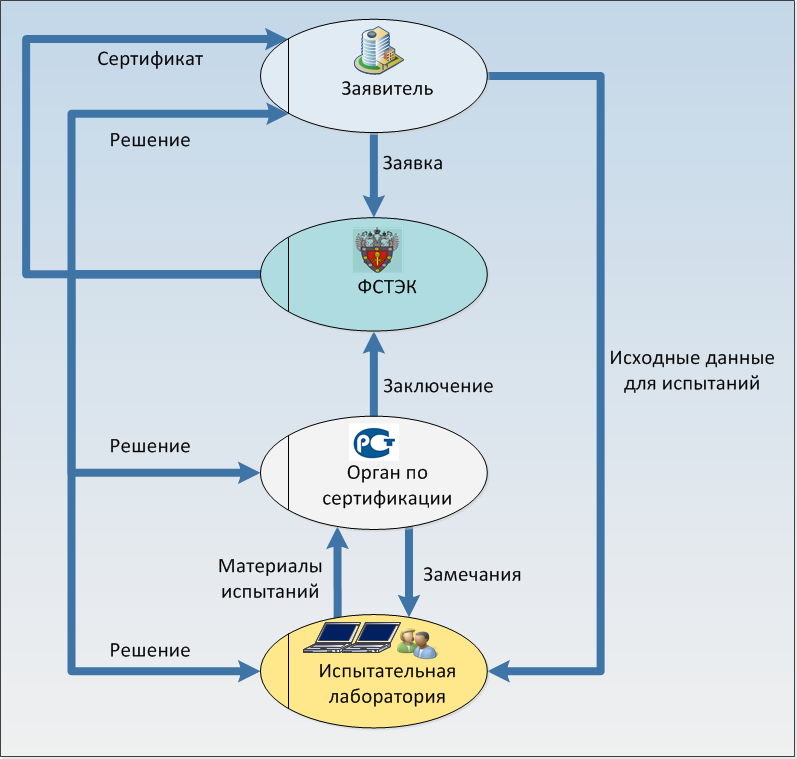
\includegraphics[width=\linewidth]{images/certification.png}
    }
    \caption{Процесс сертификации программного обеспечения во ФСТЭК\label{fig:fstak-cert}}
\end{figure}

Но существуют опасения, возникающие не на пустом месте,
что на любом из этапов сборки программы из
исходных кодов, в ней может появиться программная 
закладка \autocite{compile-a-virus, ken-thompson-hack}

Чтобы подобные ситуации исключить, применяется техника статического 
анализа исходных кодов, динамического анализа -- анализа пройденных 
программой трасс и последующее сравнение результатов обоих анализов.

На данный момент не существует открытых программных решений,
позволяющих проводить сертификацию программного обеспечения в описанном ранее формате.
Самое близкое по назначению ПО это статические анализаторы \autocite{c-static-analysis},
и так использующиеся как составная часть в процессе сертификации.
Помимо них существует свободное программное обеспечение от корпорации Microsoft --
Microsoft Application Inspector \autocite{microsoft-application-inspector}, но оно
взаимодействует только с исходными кодами программы, распознавая паттерны и назначение
функций.
Помимо свободных программ существует утилита анализа ядра Linux от ООО Фирма <<Анкад>>. 
В ней проводится статический, динамический и сравнительные анализы, но программа не умеет
работать с чем либо, кроме ядра Linux и сертифицировать что-либо еще с помощью нее не получится.
ООО Фирма <<Анкад>> на \autoref{fig:fstak-cert} выступает испытательной лабораторией.

\begin{figure}[!htbp]
    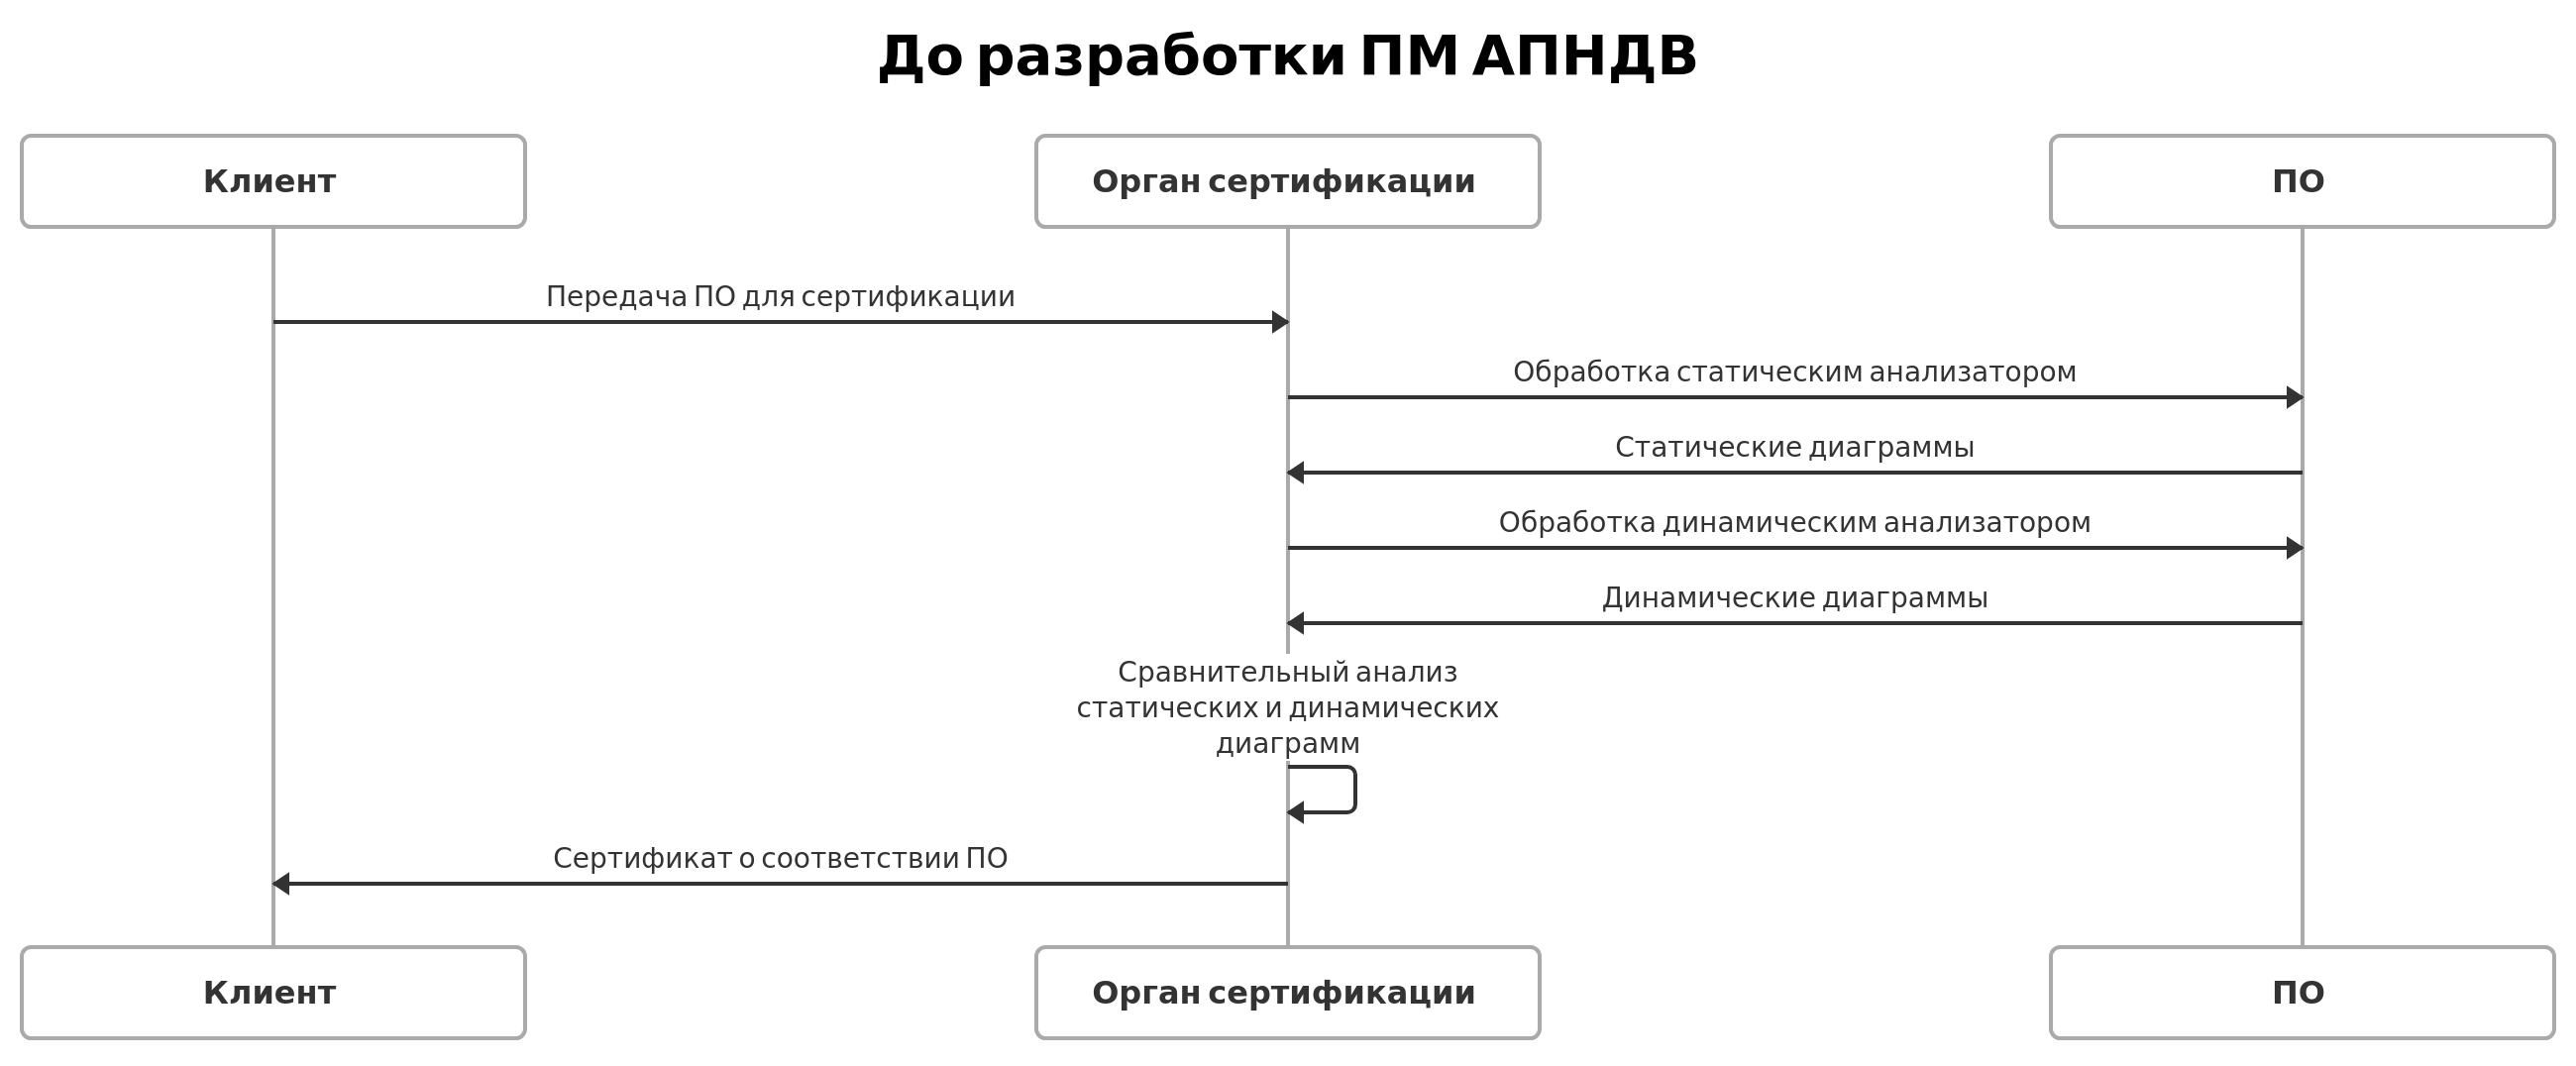
\includegraphics[width=\textwidth,height=\textheight,keepaspectratio]{images/uml_before_cropped.png}
    \caption{Процесс проведения сертификации раньше\label{fig:how-cert-was-before}}
\end{figure}

Получается, что на рынке невозможно найти комбинированных решений, 
с помощью которых было бы возможно провести процесс сертификации любого ПО. 
Для каждого конкретного проекта приходится использовать различные статические анализаторы, 
динамические анализаторы, что приводит к дублированию, по своей сути, кода и выполняемых действий, которые нужны для сертификации ПО.
Это ведет к разрастанию кодовой базы компании и нарастающим трудностям в последующей поддержке
каждого отдельного решения, что в свою очередь ведет к увеличению затрат компании.

Чтобы унифицировать разрабатываемое ПО для сертификации, было решено разбить {\ProgModule}
на модули, разделенные по ответственности и не знающие друг о друге. Это обеспечивает
удобство в редактировании, замене и изменении модулей, а при сохранении формата выдаваемой информации
 -- инкапсуляцию изменений только на конкретном модуле.

Так как модули не знают друг о друге, то и работают они в условиях ограниченной информации.
Модуль статического анализа обрабатывает только исходные коды, выдавая список статических
вызовов. Модуль динамического анализа работает с программой без отладочных символов,
собирая информацию на уровне машинных инструкций.

Данный подход помогает приблизить процесс сертификации к <<боевым>> условиям.

\ifsynopsis
Этот абзац появляется только в~автореферате.
Для формирования блоков, которые будут обрабатываться только в~автореферате,
заведена проверка условия \verb!\!\verb!ifsynopsis!.
Значение условия задаётся в~основном файле документа (\verb!synopsis.tex! для
автореферата).
\else
% Этот абзац появляется только в~диссертации.
% Через проверку условия \verb!\!\verb!ifsynopsis!, задаваемого в~основном файле
% документа (\verb!dissertation.tex! для диссертации), можно сделать новую
% команду, обеспечивающую появление цитаты в~диссертации, но~не~в~автореферате.
\fi

% {\progress}
% Этот раздел должен быть отдельным структурным элементом по
% ГОСТ, но он, как правило, включается в описание актуальности
% темы. Нужен он отдельным структурынм элемементом или нет ---
% смотрите другие диссертации вашего совета, скорее всего не нужен.

{\aim} данной работы является ускорение проведения процесса сертификации
программ написанных на языках программирования C/C++.

Для~достижения поставленной цели необходимо решить следующие {\tasks}:
\begin{enumerate}[label={\arabic*)}]
  \item анализ текущих программных решений для проведения 
        статического и динамического анализа, 
        выбор наиболее подходящего в плане универсальности 
        и расширяемости;
  \item анализ языков программирования для выбора наиболее производительного,
        надежного и легкоподдерживаемого;
  \item разработка алгоритма работы программы;
  \item разработка структур данных;
  \item разбиение функционала {\ProgModule} на модули по ответственности;
  \item разработка алгоритма передачи данных между модулями.
\end{enumerate}


% {\novelty}
% \begin{enumerate}
%   \item Впервые \ldots
%   \item Впервые \ldots
%   \item Было выполнено оригинальное исследование \ldots
% \end{enumerate}

{\influence} проекта состоит в унификации процесса сертификации ПО на отсутствие НДВ.

\begin{figure}[!htbp]
    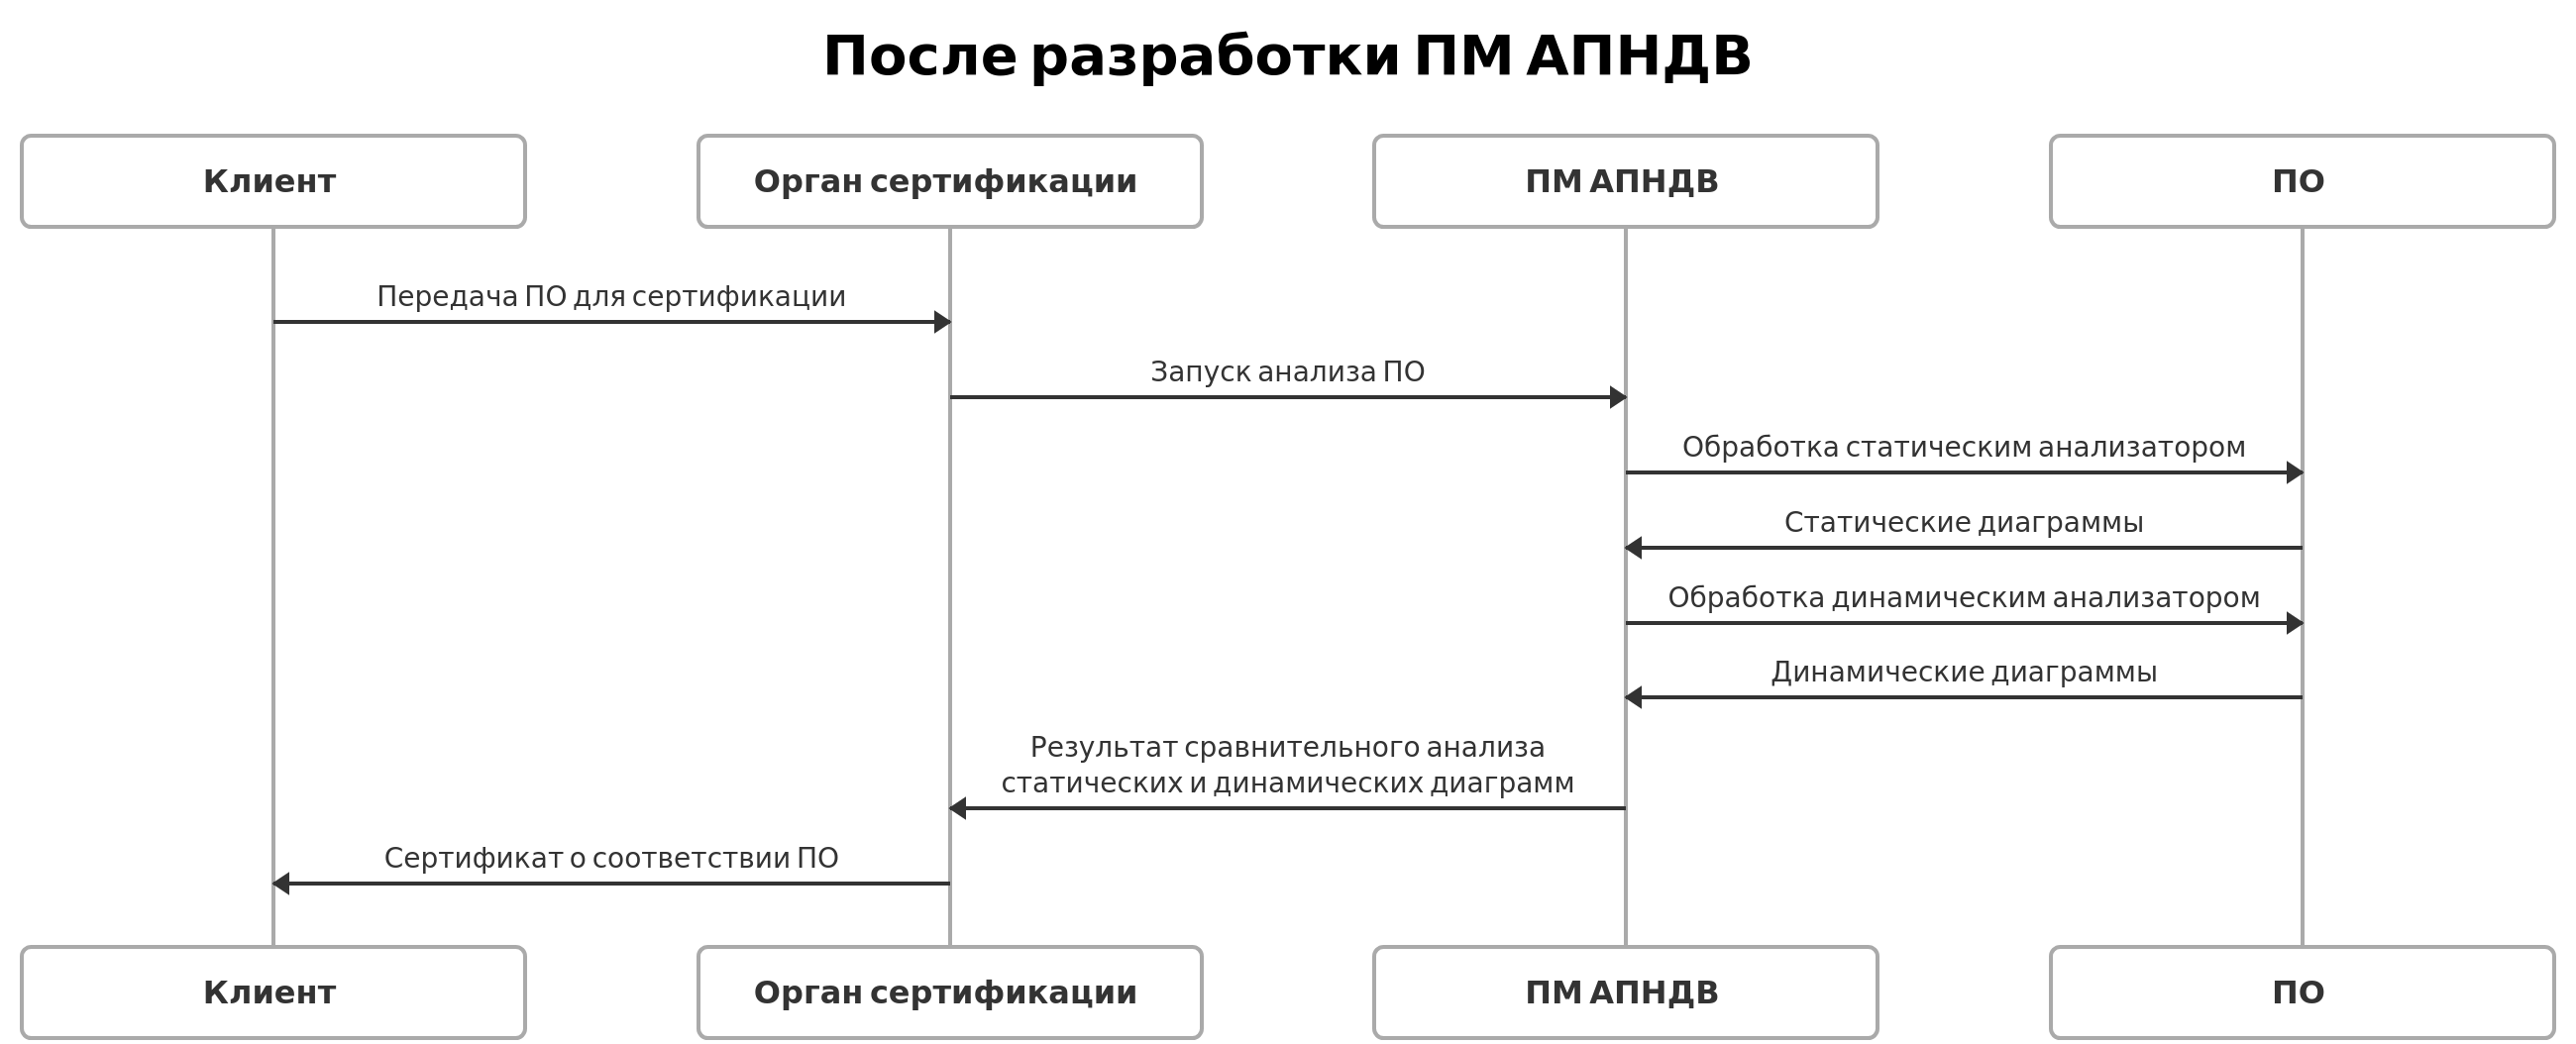
\includegraphics[width=\textwidth,height=\textheight,keepaspectratio]{images/uml_after_cropped.png}
    \caption{Процесс проведения сертификации сейчас\label{fig:how-cert-is-now}}
\end{figure}

%{\methods} \ldots

%{\defpositions}
%\begin{enumerate}
%  \item Первое положение
%\end{enumerate}
%В папке Documents можно ознакомиться в решением совета из Томского ГУ
%в~файле \verb+Def_positions.pdf+, где обоснованно даются рекомендации
%по~формулировкам защищаемых положений.

% {\reliability} полученных результатов обеспечивается \ldots \ Результаты находятся в соответствии с результатами, полученными другими авторами.
% 
% 
% {\probation}
% Основные результаты работы докладывались~на:
% перечисление основных конференций, симпозиумов и~т.\:п.
% 
% {\contribution} Автор принимал активное участие \ldots
% 
% \ifnumequal{\value{bibliosel}}{0}
% {%%% Встроенная реализация с загрузкой файла через движок bibtex8. (При желании, внутри можно использовать обычные ссылки, наподобие `\cite{vakbib1,vakbib2}`).
%     {\publications} Основные результаты по теме диссертации изложены в XX печатных изданиях,
%     X из которых изданы в журналах, рекомендованных ВАК,
%     X "--- в тезисах докладов.
% }%
% {%%% Реализация пакетом biblatex через движок biber
%     \begin{refsection}[bl-author]
%         % Это refsection=1.
%         % Процитированные здесь работы:
%         %  * подсчитываются, для автоматического составления фразы "Основные результаты ..."
%         %  * попадают в авторскую библиографию, при usefootcite==0 и стиле `\insertbiblioauthor` или `\insertbiblioauthorgrouped`
%         %  * нумеруются там в зависимости от порядка команд `\printbibliography` в этом разделе.
%         %  * при использовании `\insertbiblioauthorgrouped`, порядок команд `\printbibliography` в нём должен быть тем же (см. biblio/biblatex.tex)
%         %
%         % Невидимый библиографический список для подсчёта количества публикаций:
%         \printbibliography[heading=nobibheading, section=1, env=countauthorvak,          keyword=biblioauthorvak]%
%         \printbibliography[heading=nobibheading, section=1, env=countauthorwos,          keyword=biblioauthorwos]%
%         \printbibliography[heading=nobibheading, section=1, env=countauthorscopus,       keyword=biblioauthorscopus]%
%         \printbibliography[heading=nobibheading, section=1, env=countauthorconf,         keyword=biblioauthorconf]%
%         \printbibliography[heading=nobibheading, section=1, env=countauthorother,        keyword=biblioauthorother]%
%         \printbibliography[heading=nobibheading, section=1, env=countauthor,             keyword=biblioauthor]%
%         \printbibliography[heading=nobibheading, section=1, env=countauthorvakscopuswos, filter=vakscopuswos]%
%         \printbibliography[heading=nobibheading, section=1, env=countauthorscopuswos,    filter=scopuswos]%
%         %
%         \nocite{*}%
%         %
%         {\publications} Основные результаты по теме диссертации изложены в~\arabic{citeauthor}~печатных изданиях,
%         \arabic{citeauthorvak} из которых изданы в журналах, рекомендованных ВАК\sloppy%
%         \ifnum \value{citeauthorscopuswos}>0%
%             , \arabic{citeauthorscopuswos} "--- в~периодических научных журналах, индексируемых Web of~Science и Scopus\sloppy%
%         \fi%
%         \ifnum \value{citeauthorconf}>0%
%             , \arabic{citeauthorconf} "--- в~тезисах докладов.
%         \else%
%             .
%         \fi
%     \end{refsection}%
%     \begin{refsection}[bl-author]
%         % Это refsection=2.
%         % Процитированные здесь работы:
%         %  * попадают в авторскую библиографию, при usefootcite==0 и стиле `\insertbiblioauthorimportant`.
%         %  * ни на что не влияют в противном случае
%         \nocite{vakbib2}%vak
%         \nocite{bib1}%other
%         \nocite{confbib1}%conf
%     \end{refsection}%
%         %
%         % Всё, что вне этих двух refsection, это refsection=0,
%         %  * для диссертации - это нормальные ссылки, попадающие в обычную библиографию
%         %  * для автореферата:
%         %     * при usefootcite==0, ссылка корректно сработает только для источника из `external.bib`. Для своих работ --- напечатает "[0]" (и даже Warning не вылезет).
%         %     * при usefootcite==1, ссылка сработает нормально. В авторской библиографии будут только процитированные в refsection=0 работы.
%         %
%         % Невидимый библиографический список для подсчёта количества внешних публикаций
%         % Используется, чтобы убрать приставку "А" у работ автора, если в автореферате нет
%         % цитирований внешних источников.
%         % Замедляет компиляцию
%     \ifsynopsis
%     \ifnumequal{\value{draft}}{0}{
%       \printbibliography[heading=nobibheading, section=0, env=countexternal,          keyword=biblioexternal]%
%     }{}
%     \fi
% }
% 
% При использовании пакета \verb!biblatex! будут подсчитаны все работы, добавленные
% в файл \verb!biblio/author.bib!. Для правильного подсчёта работ в~различных
% системах цитирования требуется использовать поля:
% \begin{itemize}
%         \item \texttt{authorvak} если публикация индексирована ВАК,
%         \item \texttt{authorscopus} если публикация индексирована Scopus,
%         \item \texttt{authorwos} если публикация индексирована Web of Science,
%         \item \texttt{authorconf} для докладов конференций,
%         \item \texttt{authorother} для других публикаций.
% \end{itemize}
% Для подсчёта используются счётчики:
% \begin{itemize}
%         \item \texttt{citeauthorvak} для работ, индексируемых ВАК,
%         \item \texttt{citeauthorscopus} для работ, индексируемых Scopus,
%         \item \texttt{citeauthorwos} для работ, индексируемых Web of Science,
%         \item \texttt{citeauthorvakscopuswos} для работ, индексируемых одной из трёх баз,
%         \item \texttt{citeauthorscopuswos} для работ, индексируемых Scopus или Web of~Science,
%         \item \texttt{citeauthorconf} для докладов на конференциях,
%         \item \texttt{citeauthorother} для остальных работ,
%         \item \texttt{citeauthor} для суммарного количества работ.
% \end{itemize}
% % Счётчик \texttt{citeexternal} используется для подсчёта процитированных публикаций.
% 
% Для добавления в список публикаций автора работ, которые не были процитированы в
% автореферате требуется их~перечислить с использованием команды \verb!\nocite! в
% \verb!Synopsis/content.tex!.
 % Характеристика работы по структуре во введении и в автореферате не отличается (ГОСТ Р 7.0.11, пункты 5.3.1 и 9.2.1), потому её загружаем из одного и того же внешнего файла, предварительно задав форму выделения некоторым параметрам

\textbf{Объем и структура работы:}

Диссертация состоит из~введения, трёх глав,
заключения и~двух приложений.
% на случай ошибок оставляю исходный кусок на месте, закомментированным
Полный объём диссертации составляет  \ref*{TotPages}~страницу
с~\totalfigures{}~рисунками и~\totaltables{}~таблицами. Список литературы
содержит \total{citenum}~наименований.

    % Введение
\ifnumequal{\value{contnumfig}}{1}{\counterwithout{figure}{chapter}
}{\counterwithin{figure}{chapter}}
\ifnumequal{\value{contnumtab}}{1}{\counterwithout{table}{chapter}
}{\counterwithin{table}{chapter}}

\chapter{Создание аппаратного обеспечения}\label{ch:ch1}

В представлении обывателя компьютер (системный блок) состоит из материнской платы,
процессора, оперативной памяти, возможно видеокарты.
Давно прошли те времена, когда пользователям компьютеров приходилось отдельно покупать такие модули расширения,
как, например, математический сопроцессор.
С течением времени все больше ранее внешних модулей становится частью материнской платы или самого процессора.

Но производство аппаратного обеспечения не ограничивается потребительским рынком.
Специфические аппаратные решения требуются отдельным отраслям или организациям.

Создание аппаратного обеспечения трудоемкий процесс, непременно сязанный с созданием прикладного программного обеспечения.
В свою очередь, отсутствие возможности исполнения ПО с использованием АО серьезно усложняет отладку и тестирование конечного продукта.

\section{Эмуляция аппаратного обеспечения}\label{sec:ch1/sec1}

Тезис Чёрча-Тьюринга гласит: любая вычислимая (то есть та,
которая может быть реализована на машине Тьюринга) функция вычислима машиной Тьюринга.
Физический тезис Чёрча-Тьюринга гласит: любая функция, которая может быть вычислена физическим устройством, может быть вычислена машиной Тьюринга.

Существуют различное отношение к тезису Чёрча-Тьюринга.
Некоторые считают, что он может быть доказан, другие говорят, что он служит определением вычислений.
Не смотря на то, что тезис до сих пор не доказан, его верность исходит из того, что любая, открытая на текущий момент
реалистичная модель вычислений доказывала его правоту.

Тезис неразрывно связан с термином "эмуляция".

Эмуляция -- это процесс имитирование поведения одного оборудования и/или программного обеспечения
на другом оборудовании и/или программном обеспечении.

Эмулятор АО может использоваться как для имитирования совершенно другого оборудования, так и того, на котором она проводится.
Например, большое количество принтеров умеет эмулировать линейку LaserJet компании Hewlett-Packard,
так как большая часть ПО разработана как раз под LaserJet.

Эмуляторы аппаратного обеспечения бывают разного назначения:

\paragraph{Симуляторы логики}\label{logic-sim}

Данный вид эмуляторов используется для исследования и верификации аппаратного обеспечения на различных уровнях:
\begin{itemize}
    \item компонентном;
    \item логических вентилей;
    \item регистровых передач;
\end{itemize}

\paragraph{Высокоуровневые эмуляторы}\label{high-level-emu}

Высокоуровневая эмуляция -- это набор методов эмулирования некоторых компонентов целой системы.
Позволяет не исполнять инструкции или производить обработку данных один в один, как на целевом оборудовании,
заменяя "горячие" пути обработки аналогичными по результату.

Одними из первых данный подход был использован в эмуляторах игровых консолей, где команды отрисовки трёхмерной сцены
эмулировались не на процессоре, как все остальное оборудование консоли, а отдавались напрямую
графическому процессору машины, на которой происходил процесс эмуляции.


\paragraph{Эмуляторы процессора}\label{cpu-emu}

Эмулируют конкретную архитектуру процессора, позволяя запускать программы, не предназначенные для физического компьютера.
Зачастую умеют эмулировать не только процессор но и переферийные устройства.


\paragraph{Эмуляторы терминала}\label{term-emu}

Эмулируют терминал компьютера внутри некоторой архитектуры отображения данных на дисплее.


\paragraph{Сэмуляторы}\label{sim-emu}

Являются симбиозом симуляторов и эмуляторов, который берет лучшее от двух миров.
Аппаратное обеспечение описовается HDL языками, после чего данное описание оборудования симулируется на стендах.
Первоначальная функциональная верификация производится через симуляцию на уровне регистровых передач или логических вентилей.
В событийно-ориентированной симуляции инструкции последовательно исполняются процессором, потому что в превалирующем большинстве
сценариев не возможно провести данную симуляцию параллельно. Последовательных подход приводит к долгим симуляциям, особенно в
сложных системах на кристалле.
После симуляции описание регистровых передач должно быть зашито в аппаратное обеспечение (FPGA, ASIC).
Но идеализированное представление аппаратного обеспечения в симуляции отличается от реального аппаратного обеспечения.
Отличие между симуляцией и работой аппаратного обеспечения является серьезной причиной применений эмуляции при
проектировании.
Преимуществом данного метода является:
\begin{itemize}
    \item ускорение симуляции: часть сложной системы, не релевантная для симуляции переносится в эмулятор,
          что позволяет вынести из симуляции нерелевантные части;
    \item использование реального аппаратного обеспечения на ранних этапах проектирования;
\end{itemize}


\section{Аппаратное обеспечение -- физическое и виртуальное}\label{sec:ch1/sec2}

Прикладная польза от эмуляции аппаратного обеспечения может быть достигнута не только
при проектировании и разработке специализированного аппаратного обеспечения, но и, напрмер,
для совместного использования одного физического устройства несколькими компьютерами (в основном
виртуальными машинами).
Представляя аппаратное обеспечение гостевой системе как физическим устройство, можно
свести на нет затраты на написание специализированных драйверов и утилизировать
существующие, вынося обработку совместного использования в реализацию эмулируемого аппаратного обеспечения.

Например, можно запустить некоторое количество виртуальных машин на одной физической, и для каждой
виртуальной машины использование графического ускорителя будет прозрачным, тогда как на самом
деле управлением задачами отрисовки или обработки данных будет заниматься виртуальное устройство.

Также вынесение интерфейса реального устройства в виртуальное позволяет применить общение с программой-посредником,
которая будет отдавать команды реальному устройству или группе устройств.
Например, запускать в виртуальной машине вычисления на виртуальных графических ускорителях, которые
будут, в свою очередь, отдавать задачи обсчета реальным графическим ускорителям где-нибудь в облаке.

Помимо перечисленных выше применений, виртуальные устройства предоставляются некоторыми компаниями
в режиме PaaS -- Platform as Service или "Платформа как услуга", что позволяет другим разработчикам
испльзовать их для удаленного тестирования своих приложений в разных окружениях \cite{lambdatest} \cite{genymotion}.


\section{Создание эмуляторов}\label{sec:ch1/sec3}

Создание эмуляторов -- трудоемкий и затратный процесс. Помимо перечисленных ранее типов эмуляторов особой популярностью
пользуются так же эмуляторы игровых приставок, как старых, так и новых.
Их создание помогает сохранить игры и программы для будущих поколений, формируя целые виртуальные библиотеки, как,
например "Internet Archive"\cite{console-archive}.
С ростом вычислительной мощности усложняется и архитектура современных игровых приставок.
Эмулятор для PlayStation 4 вышел только через восемь лет после выхода самой консоли \cite{ps4-emulator}, и то
он не может запустить всю коллекцию игр, а PlayStation 4 не принадлежит последнему поколению приставок.

Создание эмуляторов какого-либо аппаратного обеспечения укладывается в следующих этапах:

\begin{figure}[!htbp]
    \centering
    \begin{tikzpicture}[%
        start chain=going below,    % General flow is top-to-bottom
        node distance=6mm and 30mm, % Global setup of box spacing
        line/.style={draw, -latex'},
        every join/.style={line},
        block/.style={draw,
                      on chain,
                      on grid,
                      rectangle,
                      minimum height = 2em}
        ]
            \node [block] (subset)
                          {вычленение эмулируемого подмножества функционала устройства};
            \node [block, fill=yellow] (conversation) [below=2cm of subset]
                          {выбор и написание средства общения ПО с эмулятором};
            \node [block] (logic) [below=2cm of conversation]
                          {написание логики эмулятора};

            \draw [line] (subset) -- (conversation);
            \draw [line] (conversation) -- (logic);

    \end{tikzpicture}
    \caption{Этапы создания эмулятора аппаратного обеспечения\label{fig:emu-creation-naive}}
\end{figure}

%\begin{enumerate}[label={\arabic*)}]
%    \item вычленения эмулируемого подмножества функционала устройства;
%    \item выбора и написания средства общения ПО с эмулятором;
%    \item .
%\end{enumerate}

Первый этап является проектировочным и его результат зависит от нужд конкретной реализации, временных ограничений,
соображений о целесообразности.
Второй этап тоже, до некоторой степени, проектировочный, но уже здесь можно принять решение
воспользоваться эмуляторами, которые поддерживают встраивание виртуального аппаратного обеспечения,
что автоматически решит задачу.
Третий этап является полностью практическим.

Облегчить второй и третий этап можно, если решить использовать уже имеющуюся инфраструктуру эмулятора,
встроив в нее эмулируемое аппаратное обеспечение.
Использование имеющейся инфраструктуры задает строгий интерфейс встраивания, что ограничивает и тривиализирует
общение ПО с виртуальным устройством.
Помимо этого, интерфейс встраивания позволяет автоматически генерировать если не всю, то часть взаимодействия
между виртуальным устройством и эмулятором.

Используя данный подход, задача создания эмулятора аппаратного обеспечения трансформируется в следующие этапы:
\begin{figure}[!htbp]
    \centering
    \begin{tikzpicture}[%
        start chain=going below,    % General flow is top-to-bottom
        node distance=6mm and 30mm, % Global setup of box spacing
        line/.style={draw, -latex'},
        every join/.style={line},
        block/.style={draw,
                      on chain,
                      on grid,
                      rectangle,
                      minimum height = 2em}
        ]
            \node [block] (subset)
                          {вычленение эмулируемого подмножества функционала устройства};
            \node [block, fill=yellow] (conversation) [below=2cm of subset]
                          {реализация общения виртуального аппаратного обеспечения и эмулятора};
            \node [block, fill=yellow] (driver) [below=2cm of conversation]
                          {реализация общения ПО с эмулятором (написание драйвера)};
            \node [block] (logic) [below=2cm of driver]
                          {написание логики эмулятора};

            \draw [line] (subset) -- (conversation);
            \draw [line] (conversation) -- (logic);
            \draw [line] (logic) -- (driver);
            \draw [line] (driver) -- (logic);

    \end{tikzpicture}
    \caption{Этапы создания эмулятора аппаратного обеспечения с использованием существующего эмулятора\label{fig:emu-creation-pro}}
\end{figure}

%\begin{enumerate}[label={\arabic*)}]
%    \item вычленения эмулируемого подмножества функционала устройства;
%    \item реализация общения виртуального аппаратного обеспечения и эмулятора;
%    \item реализация общения ПО с эмулятором (написание драйвера);
%    \item написание логики эмулятора.
%\end{enumerate}

Не смотря на увеличение количества этапов, второй и третий этап данной схемы реализовать проще и
целесообразнее, чем второй этап предыдущей схемы, так как во первом случае
протокол общения прикладного ПО и аппаратного обеспечения будет находиться частично в
эмуляторе аппаратного обеспечения, частично в прикладном ПО.
Тогда как во втором случае протокол это реализации драйвера устройства, который в любом случае придется писать.

Но даже в таком подходе можно облегчить второй и четвертый этапы, для этого не хватает только
генератора, который мог бы самостоятельно встроить будущее виртуальное аппаратное обеспечение
в эмулятор, основываясь на спецификации устройства.
Существование такого генератора не только полностью бы убрало второй этап, но и облегчило последний.
В случае, если есть возможность получить описание работы эмулируемого аппаратного обеспечения на HDL языке,
то четвертый этап создания эмулятора тоже автоматизируется, так как логика работы аппаратного обеспечения
уже описана на HDL языке.
           % Глава 1
\chapter{Формализация процесса создания эмуляторов аппаратного обеспечения}\label{ch:ch2}

Помимо сказанного в главе \ref{sec:ch1/sec4} для создании эмуляторов аппаратного обеспечения
требуется формализовать данную задачу.

\section{Подход}\label{sec:ch2/sec1}

Подход к решению обозначенных проблем будет основываться на эмуляторе QEMU и его
возможности встраивать пользовательские устройства.
Для этого необходимо:

\begin{enumerate}[label={\arabic*)}]
    \item \label{q-inh} проанализировать цепочки наследования сущностей QOM;
    \item \label{q-inh-scheme} составить схему наследования сущностей;
    \item \label{q-interface} определить интерфейс взаимодействия эмулятора с выделенными сущностями;
    \item \label{q-impl} реализовать устройство;
\end{enumerate}

Корректность выполнения пунктов \ref{q-inh}-\ref{q-interface} должна полностью брать на себя разрабатываемая система,
тогда как вместо предоставления автосгенерированного файла с исходным кодом \ref{sec:ch1/sec2} для
последующей модификации, результатом выполнения пункта \ref{q-impl} должен быть готовый к встраиванию
файл с исходным кодом, не требующий ручной модификации.
Для этого требуется проблемно-ориентированный язык, компиляция которого, помимо генерации шаблонного кода
создаст интерфейс передачи объектов между C-устройством внутри QEMU и интерпретатором Python, в
котором будет исполняться реализованная логика работы устройства.

С учетом всего вышесказанного, На рис. \ref{fig:device-compilation} показана функциональная схема преобразования
описания виртуального устройства в часть эмулятора QEMU.

\begin{figure}[!htbp]
    \centering
    % !TEX encoding = UTF-8 Unicode
% Úτƒ-8 encoded
% http://www.linux.org.ru/forum/general/10357036
\tikzset{
    line/.style={draw, -latex'},
    every join/.style={line},
    u/.style={anchor=south},
    r/.style={anchor=west},
    fxd/.style={text width = 6em},
    it/.style={font={\small\itshape}},
    bf/.style={font={\small\bfseries}},
}
\tikzstyle{base_long} =
    [
        draw,
        on chain,
        on grid,
        align=center,
        minimum height=4ex,
        minimum width = 10ex,
        node distance = 6mm and 60mm,
        text badly centered,
    ]
\tikzstyle{base} =
    [
        draw,
        on chain,
        on grid,
        align=center,
        minimum height=4ex,
        minimum width = 10ex,
        node distance = 6mm and 60mm,
        text badly centered,
        text width=5cm
    ]
\tikzstyle{coord} =
    [
        coordinate,
        on chain,
        on grid
    ]
\tikzstyle{cloud} =
    [
        base,
        ellipse,
        node distance = 3cm,
        minimum height = 2em,
        text width=2cm
    ]
\tikzstyle{decision} =
    [
        base,
        diamond,
        aspect=2,
        node distance = 2cm,
        inner sep = 0pt
    ]
\tikzstyle{block} =
    [
        rectangle,
        base,
        rounded corners,
        minimum height = 2em
    ]
\tikzstyle{print_block} =
    [
        base,
        tape,
        tape bend top=none,
    ]
\tikzstyle{io} =
    [
        base,
        trapezium,
        trapezium left angle = 70,
        trapezium right angle = 110,
    ]
\tikzstyle{prompt} =
    [
        base,
        trapezium,
        trapezium left angle = 90,
        trapezium right angle = 80,
        shape border rotate = 90
    ]
\tikzstyle{disk file} =
    [
        base,
        cylinder,
        aspect=0.2,
    ]
\tikzstyle{process} =
    [
        rectangle,
        base,
    ]
\makeatletter
\pgfkeys{/pgf/.cd,
    subrtshape w/.initial=2mm,
    cycleshape w/.initial=2mm
}
\pgfdeclareshape{parallelshape}{
    \inheritsavedanchors[from=rectangle]
    \inheritanchorborder[from=rectangle]
    \inheritanchor[from=rectangle]{north}
    \inheritanchor[from=rectangle]{center}
    \inheritanchor[from=rectangle]{west}
    \inheritanchor[from=rectangle]{east}
    \inheritanchor[from=rectangle]{mid}
    \inheritanchor[from=rectangle]{base}
    \inheritanchor[from=rectangle]{south}
    \backgroundpath{
        \southwest \pgf@xa=\pgf@x \pgf@ya=\pgf@y
        \northeast \pgf@xb=\pgf@x \pgf@yb=\pgf@y
        \def\ppd@offset{\pgfpoint{\pgfutil@tempdima}{0ex}}
        \def\ppd@offsetm{\pgfpoint{-\pgfutil@tempdima}{0ex}}
        \pgfpathmoveto{\pgfqpoint{\pgf@xa}{\pgf@ya}}
            \pgfpathlineto{\pgfqpoint{\pgf@xb}{\pgf@ya}}
        \pgfpathclose
        \pgfpathmoveto{\pgfqpoint{\pgf@xb}{\pgf@yb}}
            \pgfpathlineto{\pgfqpoint{\pgf@xa}{\pgf@yb}}
        \pgfpathclose
    }
}
\pgfdeclareshape{subrtshape}{
    \inheritsavedanchors[from=rectangle]
    \inheritanchorborder[from=rectangle]
    \inheritanchor[from=rectangle]{north}
    \inheritanchor[from=rectangle]{center}
    \inheritanchor[from=rectangle]{west}
    \inheritanchor[from=rectangle]{east}
    \inheritanchor[from=rectangle]{mid}
    \inheritanchor[from=rectangle]{base}
    \inheritanchor[from=rectangle]{south}
    \backgroundpath{
        \southwest \pgf@xa=\pgf@x \pgf@ya=\pgf@y
        \northeast \pgf@xb=\pgf@x \pgf@yb=\pgf@y
        \pgfmathsetlength\pgfutil@tempdima{\pgfkeysvalueof{/pgf/subrtshape w}}
        \def\ppd@offset{\pgfpoint{\pgfutil@tempdima}{0ex}}
        \def\ppd@offsetm{\pgfpoint{-\pgfutil@tempdima}{0ex}}
        \pgfpathmoveto{\pgfqpoint{\pgf@xa}{\pgf@ya}}
        \pgfpathlineto{\pgfqpoint{\pgf@xb}{\pgf@ya}}
        \pgfpathlineto{\pgfqpoint{\pgf@xb}{\pgf@yb}}
        \pgfpathlineto{\pgfqpoint{\pgf@xa}{\pgf@yb}}
        \pgfpathclose
        \pgfpathmoveto{\pgfpointadd{\pgfpoint{\pgf@xa}{\pgf@yb}}{\ppd@offsetm}}
        \pgfpathlineto{\pgfpointadd{\pgfpoint{\pgf@xa}{\pgf@ya}}{\ppd@offsetm}}
        \pgfpathlineto{\pgfpointadd{\pgfpoint{\pgf@xb}{\pgf@ya}}{\ppd@offset}}
        \pgfpathlineto{\pgfpointadd{\pgfpoint{\pgf@xb}{\pgf@yb}}{\ppd@offset}}
        \pgfpathclose
    }
}
\pgfdeclareshape{cyclebegshape}{
    \inheritsavedanchors[from=rectangle]
    \inheritanchorborder[from=rectangle]
    \inheritanchor[from=rectangle]{north}
    \inheritanchor[from=rectangle]{center}
    \inheritanchor[from=rectangle]{west}
    \inheritanchor[from=rectangle]{east}
    \inheritanchor[from=rectangle]{mid}
    \inheritanchor[from=rectangle]{base}
    \inheritanchor[from=rectangle]{south}
    \backgroundpath{
        \southwest \pgf@xa=\pgf@x \pgf@ya=\pgf@y
        \northeast \pgf@xb=\pgf@x \pgf@yb=\pgf@y
        \pgfmathsetlength\pgfutil@tempdima{\pgfkeysvalueof{/pgf/cycleshape w}}
        \pgfpathmoveto{\pgfqpoint{\pgf@xa}{\pgf@ya}}
\pgfpathlineto{\pgfpointadd{\pgfpoint{\pgf@xa}{\pgf@yb}}{\pgfpoint{0ex}{-\pgfutil@tempdima}}}
\pgfpathlineto{\pgfpointadd{\pgfpoint{\pgf@xa}{\pgf@yb}}{\pgfpoint{\pgfutil@tempdima}{0ex}}}
\pgfpathlineto{\pgfpointadd{\pgfpoint{\pgf@xb}{\pgf@yb}}{\pgfpoint{-\pgfutil@tempdima}{0ex}}}
\pgfpathlineto{\pgfpointadd{\pgfpoint{\pgf@xb}{\pgf@yb}}{\pgfpoint{0ex}{-\pgfutil@tempdima}}}
\pgfpathlineto{\pgfqpoint{\pgf@xb}{\pgf@ya}}
        \pgfpathclose
    }
}
\pgfdeclareshape{cycleendshape}{
    \inheritsavedanchors[from=rectangle]
    \inheritanchorborder[from=rectangle]
    \inheritanchor[from=rectangle]{north}
    \inheritanchor[from=rectangle]{center}
    \inheritanchor[from=rectangle]{west}
    \inheritanchor[from=rectangle]{east}
    \inheritanchor[from=rectangle]{mid}
    \inheritanchor[from=rectangle]{base}
    \inheritanchor[from=rectangle]{south}
    \backgroundpath{
        \southwest \pgf@xa=\pgf@x \pgf@ya=\pgf@y
        \northeast \pgf@xb=\pgf@x \pgf@yb=\pgf@y
        \pgfmathsetlength\pgfutil@tempdima{\pgfkeysvalueof{/pgf/cycleshape w}}
        \pgfpathmoveto{\pgfqpoint{\pgf@xb}{\pgf@yb}}
\pgfpathlineto{\pgfpointadd{\pgfpoint{\pgf@xb}{\pgf@ya}}{\pgfpoint{0ex}{\pgfutil@tempdima}}}
\pgfpathlineto{\pgfpointadd{\pgfpoint{\pgf@xb}{\pgf@ya}}{\pgfpoint{-\pgfutil@tempdima}{0ex}}}
\pgfpathlineto{\pgfpointadd{\pgfpoint{\pgf@xa}{\pgf@ya}}{\pgfpoint{\pgfutil@tempdima}{0ex}}}
\pgfpathlineto{\pgfpointadd{\pgfpoint{\pgf@xa}{\pgf@ya}}{\pgfpoint{0ex}{\pgfutil@tempdima}}}
\pgfpathlineto{\pgfqpoint{\pgf@xa}{\pgf@yb}}
        \pgfpathclose
    }
}
\makeatother
\tikzstyle{subroutine} =
    [
        base,
        subrtshape,
    ]
\tikzstyle{cyclebegin} =
    [
        base,
        cyclebegshape,
    ]
\tikzstyle{cycleend} =
    [
        base,
        cycleendshape,
    ]
\tikzstyle{connector} =
    [
        base,
        circle,
    ]

\tikzstyle{parallel} =
    [
        base_long,
        parallelshape,
    ]
\begin{tikzpicture}[%
    start chain=going below,    % General flow is top-to-bottom
    node distance=6mm and 30mm, % Global setup of box spacing
    ]
        \node  [rectangle,
                base,
                dotted,
                minimum width=6cm,
                minimum height=15cm] (compile rect) at (0,-10) {};

        \node [color = blue, left = 1cm of compile rect, yshift = 0.25cm]  (group) {\small Компиляция устройства};
        \draw [color = blue, decorate, decoration = {brace,amplitude=10pt,raise=5pt, mirror}] (-3cm,-2cm) --  (-3cm,-17cm);


        \node  [cloud] (begin) at (0,0) {\small Начало};
        \node  [subroutine]   (parse)          [below = 2cm of begin]            {\small Разбор файла};
        \node  [subroutine]   (qemu inh)       [below = 2cm of parse]            {\small Поиск используемых\\сущностей QEMU};
        \node  [subroutine]   (qemu inh inter) [below = 2.2cm of qemu inh]       {\small Определение интерфейса используемых\\сущностей QEMU};
        \node  [subroutine]   (qemu inh boil)  [below = 2.2cm of qemu inh inter] {\small Генерация C-интерфейса устройства в QEMU};
        \node  [subroutine]   (python)         [below = 2.2cm of qemu inh boil]  {\small Генерация python-интерфейса\\для логики устройства};
        \node  [subroutine]   (buildsystem)    [below = 2.2cm of python]         {\small Встраивание устройства\\в сборку QEMU};

        \node  [disk file] (source)         [left  = 8cm of parse]            {\small Исходный код устройства};
        \node  [disk file] (qemu folder)    [left  = 8cm of buildsystem]      {\small Сборочная папка QEMU};
        \node  [subroutine] (compile)       [below = 3cm of buildsystem]      {\small Сборка QEMU};
        \node  [disk file] (binary)         [left  = 8cm of compile]        {\small QEMU со встроенным устройством};

        \node  [cloud] (end) [below = 2cm of compile] {\small Конец};

        \draw [->] (begin)          -- (parse);
        \draw [->] (source)         -- (parse);
        \draw [->] (parse)          -- (qemu inh);
        \draw [->] (qemu inh)       -- (qemu inh inter);
        \draw [->] (qemu inh inter) -- (qemu inh boil);
        \draw [->] (qemu inh boil)  -- (python);
        \draw [->] (python)         -- (buildsystem);
        \draw [->] (qemu folder)    -- (buildsystem);
        \draw [->] (buildsystem)    -- (compile);
        \draw [->] (compile)        -- (binary);
        \draw [->] (compile)        -- (end);


\end{tikzpicture}

    \caption{Функциональная схема компиляции виртуального устройства.}\label{fig:device-compilation}
\end{figure}


\subsection{Язык описания виртуального устройства}\label{sec:ch2/sec1/sub1}

Использование специализированного языка для описания устройства, в отличие от языка общего назначения (см. \ref{sec:ch1/sec2}),
имеет как определенные преимущества, так и недостатки.
К преимуществам можно отнести:
\begin{itemize}
    \item ограничение пользователя языка только необходимыми конструкциями -- минимизация ошибок программирования;
    \item точные, по сравнению с языком общего назначения, сообщения об ошибках;
    \item самодокументируемость решения проблемы;
    \item более эффективная, по времени, разработка.
\end{itemize}

К недостаткам -- необходимость предварительного изучения проблемно-ориентированного языка.
Как можно убедиться, преимуществ, несмотря на определенную трудоемкость разработки такого языка,
больше.
Необходимость изучения дополнительного языка для описания виртуального устройства может показаться
избыточной, но использование языка общего назначения (см. \ref{sec:ch1/sec2}),
пусть и популярного, не гарантирует, что пользователь его знает и эффективно в нем работает.
Помимо этого, изучение небольшого языка для решения конкретной проблемы будет эффективнее
изучения библиотеки и некоторого подмножества полноценного языка программирования,
из которого ее можно будет использовать.

Ограничение в языковых конструкциях и анализ семантики исходного кода
позволяет точно инструктировать пользователя об ошибках в реализации виртуального устройства,
что ведет к отсутствию ошибок уровня интерфейса устройства,
сводя появление возможных неисправностей только до реализации логики устройства.

Язык-фреймворк Racket \cite{racket-lang} разработан как раз для языково-ориентированного
программирования. Написание на нем логики компилятора или интерпретатора целевого языка
полуавтоматически создает интегрированную среду разработки с помощью IDE DrRacket, которую
также поддерживает сообщество.
После объявления некоторых функций \cite{racket-drracket-integration}, разработчик программ
на целевом языке сможет пользоваться подсветкой синтаксиса, отладчиком, автоматическим добавлением
отступов и указателями использования переменных (рис. \ref{fig:racket-variable-arrow}), что дополнительно облегчает разработку.

\begin{figure}[!htbp]
    \centering
    \begin{adjustbox}{max totalsize={\textwidth}{\textheight}}
        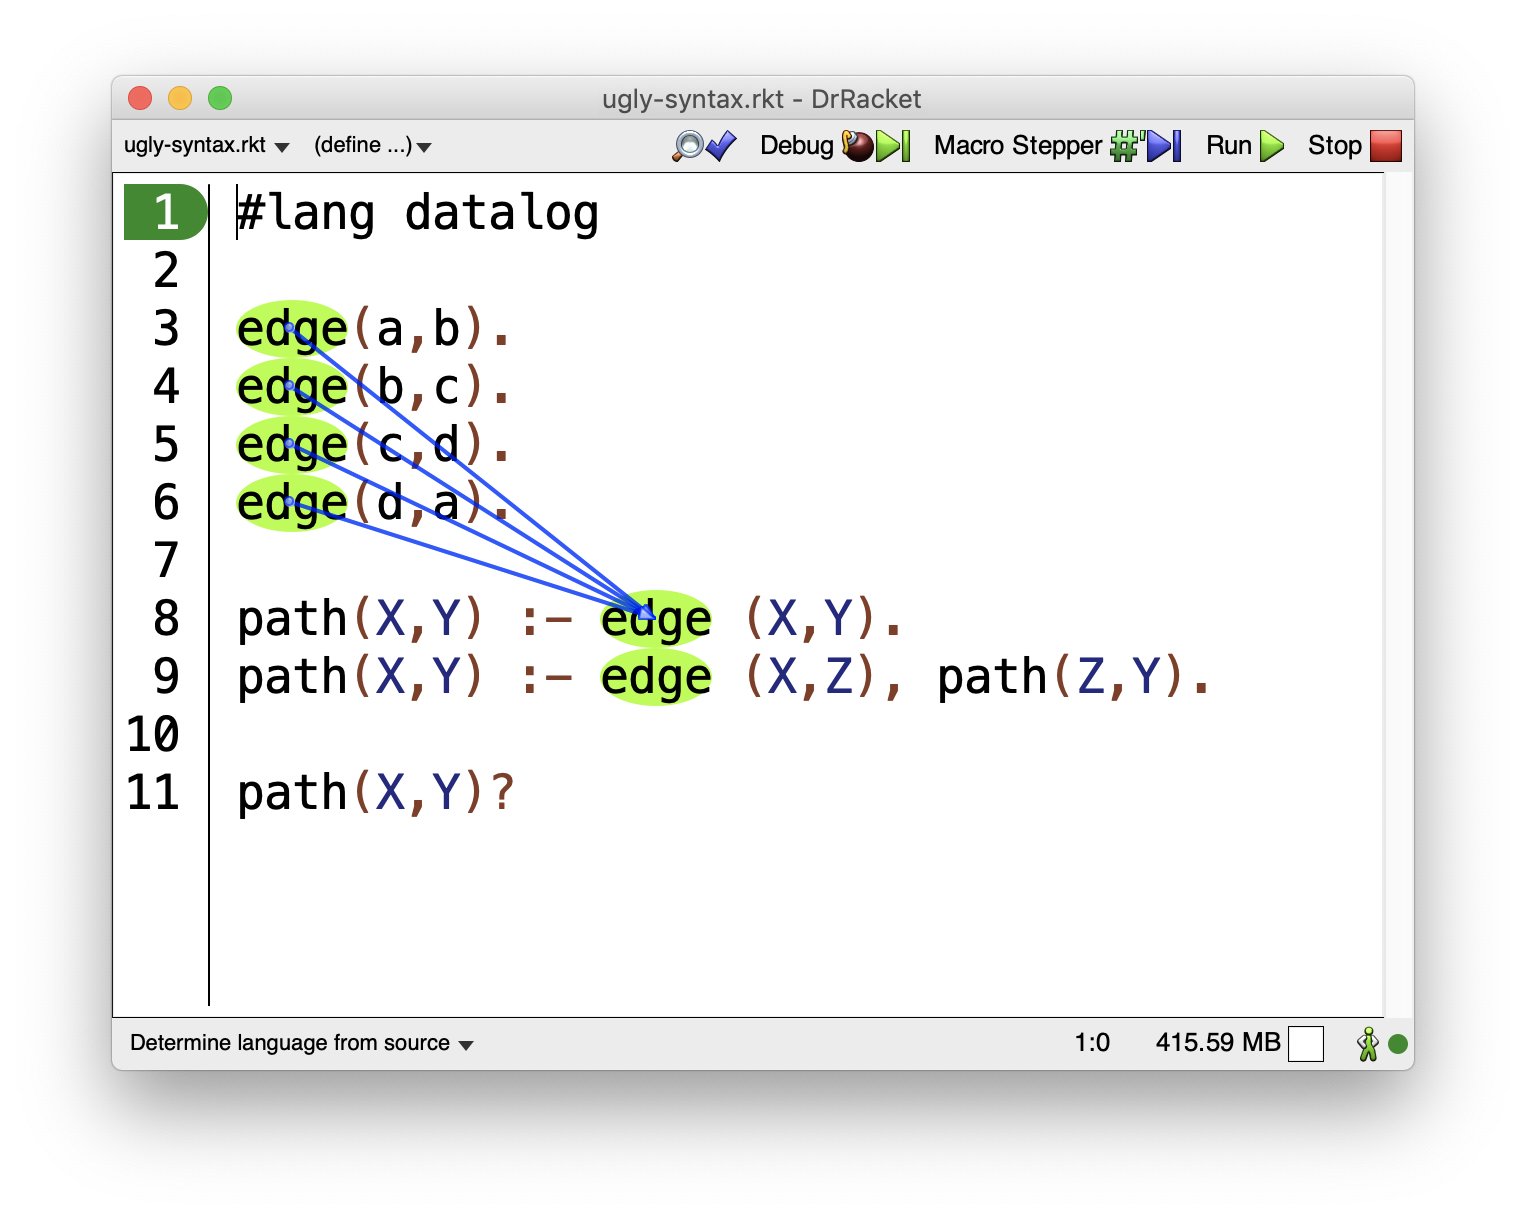
\includegraphics[]{images/racket-variable-arrow.png}
    \end{adjustbox}
    \caption{Результат интеграции языка datalog в IDE DrRacket.}\label{fig:racket-variable-arrow}
\end{figure}


\subsubsection{Структура программы}\label{sec:ch2/sec1/sub1/sub1}

Структура программы-описания аппаратного обеспечения имеет следующий вид, рисунок \ref{fig:device-program-structure}.

\begin{figure}[!htbp]
    \centering
    % !TEX encoding = UTF-8 Unicode
% Úτƒ-8 encoded
% http://www.linux.org.ru/forum/general/10357036
\tikzset{
    line/.style={draw, -latex'},
    every join/.style={line},
    u/.style={anchor=south},
    r/.style={anchor=west},
    fxd/.style={text width = 6em},
    it/.style={font={\small\itshape}},
    bf/.style={font={\small\bfseries}},
}
\tikzstyle{base_long} =
    [
        draw,
        on chain,
        on grid,
        align=center,
        minimum height=4ex,
        minimum width = 10ex,
        node distance = 6mm and 60mm,
        text badly centered,
    ]
\tikzstyle{base} =
    [
        draw,
        on chain,
        on grid,
        align=center,
        minimum height=4ex,
        minimum width = 10ex,
        node distance = 6mm and 60mm,
        text badly centered,
        text width=5cm
    ]
\tikzstyle{coord} =
    [
        coordinate,
        on chain,
        on grid
    ]
\tikzstyle{cloud} =
    [
        base,
        ellipse,
        node distance = 3cm,
        minimum height = 2em,
        text width=2cm
    ]
\tikzstyle{decision} =
    [
        base,
        diamond,
        aspect=2,
        node distance = 2cm,
        inner sep = 0pt
    ]
\tikzstyle{block} =
    [
        rectangle,
        base,
        rounded corners,
        minimum height = 2em
    ]
\tikzstyle{print_block} =
    [
        base,
        tape,
        tape bend top=none,
    ]
\tikzstyle{io} =
    [
        base,
        trapezium,
        trapezium left angle = 70,
        trapezium right angle = 110,
    ]
\tikzstyle{prompt} =
    [
        base,
        trapezium,
        trapezium left angle = 90,
        trapezium right angle = 80,
        shape border rotate = 90
    ]
\tikzstyle{disk file} =
    [
        base,
        cylinder,
        aspect=0.2,
    ]
\tikzstyle{process} =
    [
        rectangle,
        base,
    ]
\makeatletter
\pgfkeys{/pgf/.cd,
    subrtshape w/.initial=2mm,
    cycleshape w/.initial=2mm
}
\pgfdeclareshape{parallelshape}{
    \inheritsavedanchors[from=rectangle]
    \inheritanchorborder[from=rectangle]
    \inheritanchor[from=rectangle]{north}
    \inheritanchor[from=rectangle]{center}
    \inheritanchor[from=rectangle]{west}
    \inheritanchor[from=rectangle]{east}
    \inheritanchor[from=rectangle]{mid}
    \inheritanchor[from=rectangle]{base}
    \inheritanchor[from=rectangle]{south}
    \backgroundpath{
        \southwest \pgf@xa=\pgf@x \pgf@ya=\pgf@y
        \northeast \pgf@xb=\pgf@x \pgf@yb=\pgf@y
        \def\ppd@offset{\pgfpoint{\pgfutil@tempdima}{0ex}}
        \def\ppd@offsetm{\pgfpoint{-\pgfutil@tempdima}{0ex}}
        \pgfpathmoveto{\pgfqpoint{\pgf@xa}{\pgf@ya}}
            \pgfpathlineto{\pgfqpoint{\pgf@xb}{\pgf@ya}}
        \pgfpathclose
        \pgfpathmoveto{\pgfqpoint{\pgf@xb}{\pgf@yb}}
            \pgfpathlineto{\pgfqpoint{\pgf@xa}{\pgf@yb}}
        \pgfpathclose
    }
}
\pgfdeclareshape{subrtshape}{
    \inheritsavedanchors[from=rectangle]
    \inheritanchorborder[from=rectangle]
    \inheritanchor[from=rectangle]{north}
    \inheritanchor[from=rectangle]{center}
    \inheritanchor[from=rectangle]{west}
    \inheritanchor[from=rectangle]{east}
    \inheritanchor[from=rectangle]{mid}
    \inheritanchor[from=rectangle]{base}
    \inheritanchor[from=rectangle]{south}
    \backgroundpath{
        \southwest \pgf@xa=\pgf@x \pgf@ya=\pgf@y
        \northeast \pgf@xb=\pgf@x \pgf@yb=\pgf@y
        \pgfmathsetlength\pgfutil@tempdima{\pgfkeysvalueof{/pgf/subrtshape w}}
        \def\ppd@offset{\pgfpoint{\pgfutil@tempdima}{0ex}}
        \def\ppd@offsetm{\pgfpoint{-\pgfutil@tempdima}{0ex}}
        \pgfpathmoveto{\pgfqpoint{\pgf@xa}{\pgf@ya}}
        \pgfpathlineto{\pgfqpoint{\pgf@xb}{\pgf@ya}}
        \pgfpathlineto{\pgfqpoint{\pgf@xb}{\pgf@yb}}
        \pgfpathlineto{\pgfqpoint{\pgf@xa}{\pgf@yb}}
        \pgfpathclose
        \pgfpathmoveto{\pgfpointadd{\pgfpoint{\pgf@xa}{\pgf@yb}}{\ppd@offsetm}}
        \pgfpathlineto{\pgfpointadd{\pgfpoint{\pgf@xa}{\pgf@ya}}{\ppd@offsetm}}
        \pgfpathlineto{\pgfpointadd{\pgfpoint{\pgf@xb}{\pgf@ya}}{\ppd@offset}}
        \pgfpathlineto{\pgfpointadd{\pgfpoint{\pgf@xb}{\pgf@yb}}{\ppd@offset}}
        \pgfpathclose
    }
}
\pgfdeclareshape{cyclebegshape}{
    \inheritsavedanchors[from=rectangle]
    \inheritanchorborder[from=rectangle]
    \inheritanchor[from=rectangle]{north}
    \inheritanchor[from=rectangle]{center}
    \inheritanchor[from=rectangle]{west}
    \inheritanchor[from=rectangle]{east}
    \inheritanchor[from=rectangle]{mid}
    \inheritanchor[from=rectangle]{base}
    \inheritanchor[from=rectangle]{south}
    \backgroundpath{
        \southwest \pgf@xa=\pgf@x \pgf@ya=\pgf@y
        \northeast \pgf@xb=\pgf@x \pgf@yb=\pgf@y
        \pgfmathsetlength\pgfutil@tempdima{\pgfkeysvalueof{/pgf/cycleshape w}}
        \pgfpathmoveto{\pgfqpoint{\pgf@xa}{\pgf@ya}}
\pgfpathlineto{\pgfpointadd{\pgfpoint{\pgf@xa}{\pgf@yb}}{\pgfpoint{0ex}{-\pgfutil@tempdima}}}
\pgfpathlineto{\pgfpointadd{\pgfpoint{\pgf@xa}{\pgf@yb}}{\pgfpoint{\pgfutil@tempdima}{0ex}}}
\pgfpathlineto{\pgfpointadd{\pgfpoint{\pgf@xb}{\pgf@yb}}{\pgfpoint{-\pgfutil@tempdima}{0ex}}}
\pgfpathlineto{\pgfpointadd{\pgfpoint{\pgf@xb}{\pgf@yb}}{\pgfpoint{0ex}{-\pgfutil@tempdima}}}
\pgfpathlineto{\pgfqpoint{\pgf@xb}{\pgf@ya}}
        \pgfpathclose
    }
}
\pgfdeclareshape{cycleendshape}{
    \inheritsavedanchors[from=rectangle]
    \inheritanchorborder[from=rectangle]
    \inheritanchor[from=rectangle]{north}
    \inheritanchor[from=rectangle]{center}
    \inheritanchor[from=rectangle]{west}
    \inheritanchor[from=rectangle]{east}
    \inheritanchor[from=rectangle]{mid}
    \inheritanchor[from=rectangle]{base}
    \inheritanchor[from=rectangle]{south}
    \backgroundpath{
        \southwest \pgf@xa=\pgf@x \pgf@ya=\pgf@y
        \northeast \pgf@xb=\pgf@x \pgf@yb=\pgf@y
        \pgfmathsetlength\pgfutil@tempdima{\pgfkeysvalueof{/pgf/cycleshape w}}
        \pgfpathmoveto{\pgfqpoint{\pgf@xb}{\pgf@yb}}
\pgfpathlineto{\pgfpointadd{\pgfpoint{\pgf@xb}{\pgf@ya}}{\pgfpoint{0ex}{\pgfutil@tempdima}}}
\pgfpathlineto{\pgfpointadd{\pgfpoint{\pgf@xb}{\pgf@ya}}{\pgfpoint{-\pgfutil@tempdima}{0ex}}}
\pgfpathlineto{\pgfpointadd{\pgfpoint{\pgf@xa}{\pgf@ya}}{\pgfpoint{\pgfutil@tempdima}{0ex}}}
\pgfpathlineto{\pgfpointadd{\pgfpoint{\pgf@xa}{\pgf@ya}}{\pgfpoint{0ex}{\pgfutil@tempdima}}}
\pgfpathlineto{\pgfqpoint{\pgf@xa}{\pgf@yb}}
        \pgfpathclose
    }
}
\makeatother
\tikzstyle{subroutine} =
    [
        base,
        subrtshape,
    ]
\tikzstyle{cyclebegin} =
    [
        base,
        cyclebegshape,
    ]
\tikzstyle{cycleend} =
    [
        base,
        cycleendshape,
    ]
\tikzstyle{connector} =
    [
        base,
        circle,
    ]

\tikzstyle{parallel} =
    [
        base_long,
        parallelshape,
    ]
\begin{tikzpicture}[%
    start chain=going below,    % General flow is top-to-bottom
    node distance=6mm and 30mm, % Global setup of box spacing
    ]
        \node  [rectangle,
                base,
                minimum width=6cm] (device class)
                {Описание класса устройства};
        \node  [rectangle,
                base,
                minimum width=6cm] (c-python api)
                [below = 1.5cm of device class]
                {Связывание функций C-Python интерфейса};
        \node  [rectangle,
                base,
                minimum width=6cm] (py logic)
                [below = 1.85cm of c-python api]
                {Реализация логики работы устройства на Python};



\end{tikzpicture}

    \caption{Структура программы-описания аппаратного обеспечения.}\label{fig:device-program-structure}
\end{figure}

Несмотря на то, что компилятор язык программы-описания располагает
блоки кода в результирующем тексте модуле QEMU в соответствии
с правилами языка C и порядок объявления блоков в исходном файле ему не важен,
данная структура является наиболее понятной и органичной для стороннего разработчика.
Поэтому компилятор принуждает программиста придерживаться её, подобно тому, как
язык Python обязывает использовать отступы для создания блоков кода.


\subsubsection{Граммматика языка}\label{sec:ch2/sec1/sub1/sub2}
Разрабатываемый язык является языком с контекстно-свободной грамматикой.
Далее он будет именоваться как {\mylanguage} (произносится \mylanguageprononciation)

Грамматика {\mylanguage} ограничена до описания зависимостей устройства и QEMU,
связывания функций C и Python, встраивания Python-кода с логикой работы устройства
в файл.


% TODO: Учтено ли, что пользователь захочет кастомизировать функции инициализации класса и инстанса?
% TODO: MemoryRegionOps?
\begin{figure}[!htbp]
    \begin{grammar}
        <letter> ::= `a' ... `z' | `A' ... `Z';

        <digit> ::= `0' ... `9' ;

        <symbol> ::= \symbol{92}x20 ... \symbol{92}x7E ; (* любой печатный символ, согласно кодам ASCII *)

        <const value> ::= <digit> | `"' \{ <symbol> \} `"';

        <identifier> ::= <letter> [\{ <letter> | <digit> | `\_' \}] ;

        <block start> ::= `{';

        <block end> ::= `}';

        <field> ::= <identifier> `=' <identifier> | <block> ;

        <block> ::= <block start> <field> [\{ `,' <field> \}] <block end>;

        <device definition> ::= '\#' <identifier>;

        <device class inheritance> ::= `(' <identifier> `:' <identifier> [\{ `,' <identifier> \}] `)';

        <device class block> ::= <device class inheritance> <block>;

        <bind block> ::= `@bind' <block>;

        <python block> ::= `@py' <block>;

        <program> ::= <device definition> <device class block> <bind block> <python block>;
    \end{grammar}
    \caption{Расширенная форма Бэкуса-Наура \mylanguage}\label{fig:qpydev-grammar}
\end{figure}


\subsubsection{Семантика языка}\label{sec:ch2/sec1/sub1/sub3}

Для описания семантики языка {\mylanguage} была выбрана денотационная семантика.
Краеугольным камнем денотационной семантики является определение для каждой сущности
языка некоего математического объекта и некоей функции, называемой интерпретатором,
которая отображает экземпляры этой сущности в экземпляры этого математического объекта -- элемент множества денотаций.
Поскольку математические объекты строго определены, то они представляют собой точный
смысл соответствующих сущностей.

Функции обозначают посредством двойных квадратных скобок $[[$ $]]$,
а элемент алгебры или операция алгебры, сопоставленные функцией $[[$ $]]$
правильному выражению или конструктору выражений, называют денотантом этого выражения или,
соответственно, денотацией конструкции. \cite{denotational-semantics}

Для языка {\mylanguage} значимыми множествами семантических объектов
являются только множества $Q$ -- объектов QEMU (переменные, функции, структуры) и
$C$ -- множество константных выражений.


\begin{figure}[!htbp]
    \centering
    \begingroup
    \addtolength{\jot}{1em}
    \begin{gather*}
        [[assignment]](x,y) = \lambda x.y \\
        [[terminate]](m) \text{ Завершение работы компилятора} \\
        [[if]](c,e_1,e_2) =
        \begin{cases}
            e_1, & \text{Если } c = true \\
            e_2, & \text{Если } c \not= true
        \end{cases} \\
        [[throw\ error]](c, e) = if(c, e_g, terminate) \\
        [[lookup]](o) = [[throw\ error]](o \in Q, o) \\
        [[<device\ definition>]](i) = lookup(i) \\
        [[<device\ class\ inheritance>]](i_1,...,i_n) = lookup(i_1) + ... + lookup(i_n) \\
        [[<field>]](v_1, v_2) = assignment(v_1, v_2), \text{ Если } v_1 \in Q \text{ и } v_3 \in C \cup Q \\
        [[<block>]](f_1,...,f_n) = field(f_1) + ... + field(f_n) \\
        [[<python block>]](b) = assignment(B,B)\\
    \end{gather*}
    \endgroup
    \caption{Денотационная семантика {\mylanguage}}\label{fig:denotational-semantics}
\end{figure}


\subsection{Поиск используемых сущностей QEMU}\label{sec:ch2/sec1/sub2}

Пробрасывание -- процесс преобразовывания и передачи данных между двумя интерфейсами.

Поиск используемых сущностей состоит в установлении типов QEMU для последующего
корректного пробрасывания их в логику устройства.
Также это необходимо для проверки корректности наследования и встраивания устройства.
Необходимыми для пробрасывания типами являются структуры и функции, оперирующие ими.

Рекурсивное преобразование структур QEMU в типы python важно для удобного и читаемого
использования C-объектов внутри python-логики.
Пробрасывание в python функций QEMU необходимо для использования уже имеющегося API эмулятора.
% TODO: может удалить, если это сложно
Потенциально, может быть удобным использование макросов препроцессора C внутри
логики Python.

Базовым классом для всех классов QEMU является класс \texttt{Object}.
Наследование происходит через определение первым членом C-структуры
указателя на структуру-родитель данной. Так как язык C гарантирует, что
первый член структуры всегда начинается с нулевого отступа от начала
структуры, любой класс можно привести к типу Object.
В свою очередь Object содержит структуру, описывающую класс приведенного
объекта -- \texttt{ObjectClass}, что позволяет определить реальный тип указателя
во время исполнения.

Структуры \texttt{TypeImpl} и \texttt{TypeInfo} (см рис. \ref{fig:qom-structure}) практически не отличаются,
но служат для разных целей:
\texttt{TypeImpl} является <<внутренним>> содержанием класса, служебной структурой,
которая скрывает методы класса от пользователя интерфейса, тогда как \texttt{TypeInfo}
наоборот, предоставляет уже очищенный от служебных полей интерфейс для инициализации \texttt{TypeImpl}.

После объявления \texttt{TypeInfo}, структура регистрируется в объектной системе QEMU.
Это происходит через использование макроса \texttt{type\_init}, который создает, можно считать,
анонимную функцию, в свою очередь вызывающую функцию \texttt{register\_module\_init}.
Созданная анонимная функция помечается атрибутом \texttt{constructor} \cite{gcc-attributes}, что заставляет
компилятор добавить вызов такой функции до вызова функции main.
Соответственно, инициализация модулей происходит до того, как начнет исполняться логика QEMU.

% TODO: А точно ли?

Все перефирийные устройства, добавляемые в QEMU, <<общаются>> с другими устройствами через чтение и запись
по определенным для устройства адресам памяти.
За это отвечает структура \texttt{MemoryRegionOps} \ref{fig:mem-reg-ops},
которая инициализируется функциями чтения и записи,
которые вызываются, соответственно, при чтении или записи памяти, на которое <отображено>> устройство.
Данные функции принимают на вход указатель на устройство, в чью память происходит чтение или запись,
адрес, по которому происходит чтение или запись, и, в случае чтения, количество читаемых байт,
а в случае записи -- записываемое значение и количество записываемых байт.
Некоторые устройства используют расширенные версии чтения и записи, где последним аргументом передается
структура с атрибутами транзакции.

\begin{figure}[!htbp]
    \centering
    \begin{adjustbox}{max totalsize={\textwidth}{\textheight}}
        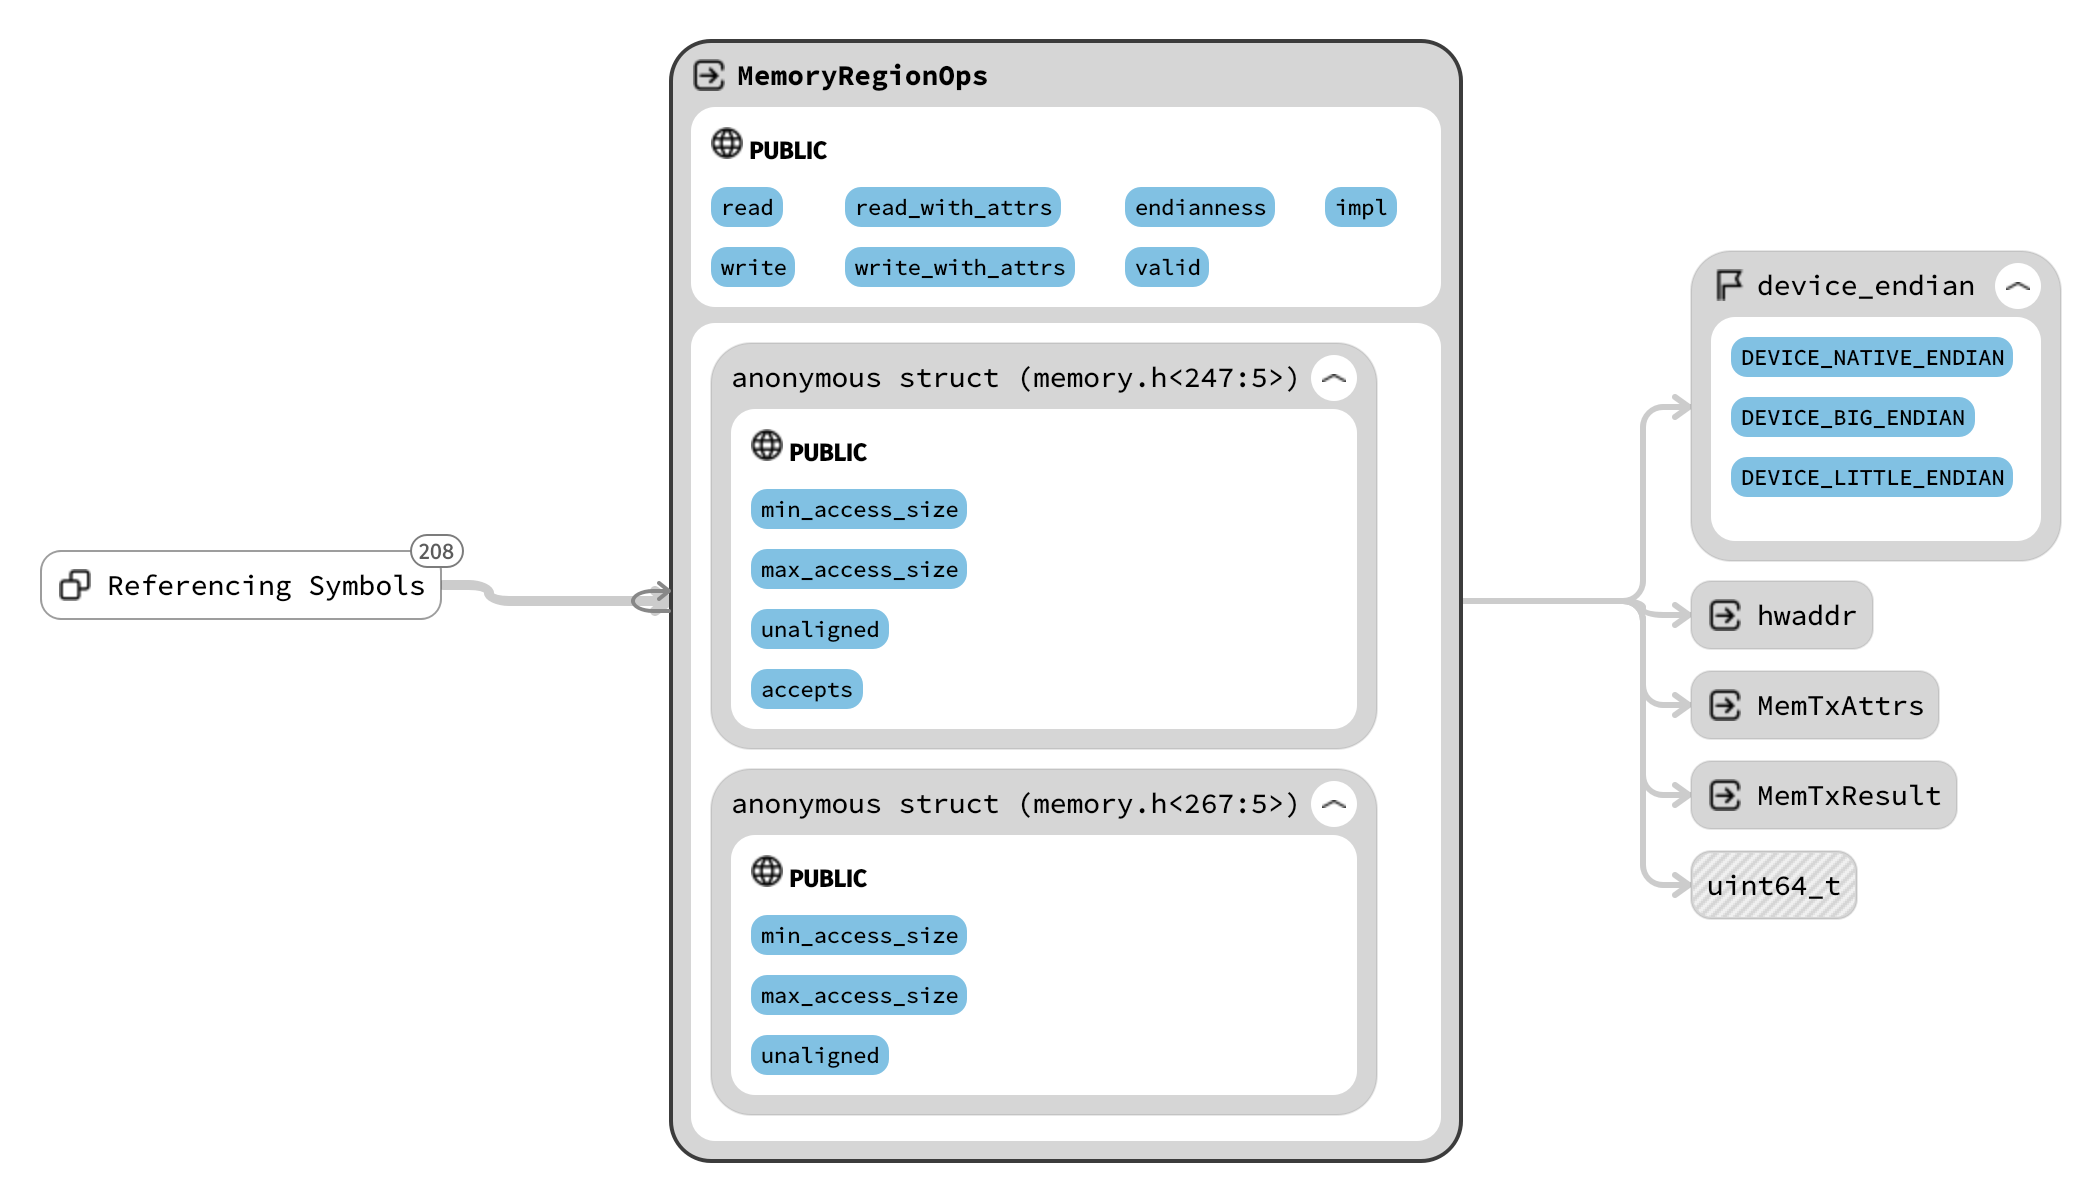
\includegraphics[]{images/mem_reg_ops_cropped.png}
    \end{adjustbox}
    \caption{Связь \texttt{MemoryRegionOps} с другими сущностями QEMU.}\label{fig:mem-reg-ops}
\end{figure}


\subsubsection{Механизм нахождения информации о типах устройств}\label{sec:ch2/sec1/sub2/sub1}

Все устройства QEMU:
\begin{enumerate}[label={\arabic*)}]
    \item имеют родителя и распределены по подпапкам папки \texttt{hw};
    \item объявляют структуру \texttt{TypeInfo}, в которой указывается родитель устройства
          и размер создаваемого объекта -- поле \texttt{.instance\_size}
          (используется для создания объектов устройств на системной шине);
    \item используют оператор \texttt{sizeof},
          передавая ему имя структуры устройства, которое будет исполняться в QEMU.
\end{enumerate}

Данная информация позволяет найти используемые сущности QEMU следующим образом:
\begin{enumerate}[label={\arabic*)}]
    \item пройтись по всем файлам, находящимся в папке \texttt{hw};
    \begin{enumerate}[label={\arabic*)}]
        \item найти структуру \texttt{TypeInfo};
        \item проанализировать поле \texttt{.instance\_size} и сохранить
              используемую структуру как возможную для наследования;
        \item сохранить поле \texttt{.name} в качестве имени структуры для наследования;
    \end{enumerate}
\end{enumerate}

Помимо явного описания структуры \texttt{TypeInfo} некоторые устройства, написанные
в современном стиле, используют макросы:
\begin{enumerate}[label={\arabic*)}]
    \item \label{main-def-macro} \texttt{OBJECT\_DEFINE\_TYPE\_EXTENDED};
    \item \texttt{OBJECT\_DEFINE\_TYPE};
    \item \texttt{OBJECT\_DEFINE\_TYPE\_WITH\_INTERFACES};
    \item \texttt{OBJECT\_DEFINE\_ABSTRACT\_TYPE}.
\end{enumerate}

Все перечисленные макросы создают структуру \texttt{TypeInfo} и все, кроме \ref{main-def-macro},
вызывают внутри себя макрос \ref{main-def-macro}, специализируя определенные поля структуры \texttt{TypeInfo}.
Например \texttt{OBJECT\_DEFINE\_ABSTRACT\_TYPE} создает абстрактный тип, передавая внутри себя
значение \texttt{true} макросу \texttt{OBJECT\_DEFINE\_TYPE\_EXTENDED}, чем облегчает собственный интерфейс
и делает свое использование более выразительным.

Список аргументов макросов объявления типов также требуется разбирать, чтобы получить из аргументов информацию
о структуре \texttt{TypeInfo}.

Механизм получения информации о функциях намного проще: в языке C функции могут инкапсулироваться
только на уровне одного модуля трансляции -- C-файла, прошедшего этап препроцессирования.
Инкапсулированные функции помечаются ключевым словом \texttt{static}, что делает их
<<невидимыми>> в других модулях трансляции.
Все функции, не помеченные ключевым словом \texttt{static} будем считать интерфейсными.

Данная информация будет использована впоследствии для корректной кодогенерации устройства
и преобразования C-структур и C-функций в читаемый вид для python-интерфейса.

\subsubsection{Механизм использования информации о типах устройств}\label{sec:ch2/sec1/sub2/sub2}

Так как код QEMU насыщен использованием макросов, потребуется инструмент для их разворачивания -- препроцессор.
Чтобы не создавать собственную имплементацию препроцессора, этим будет заниматься препоцессор системного компилятора.

Практически во всех системах сборки программ в POSIX окружении используется компилятор gcc или clang.
Оба компилятора являются совместимыми между собой. Для задействования препроцессора компилятора используется
опция \texttt{-E}. Так как препроцессор C, помимо раскрытия макросв занимается еще нахождением и подстановкой
заголовочных файлов, то потребуется указать папки с их местонахождением.
QEMU полагается на:
\begin{enumerate}[label={\arabic*)}]
    \item \label{build-header} заголовочные файлы, создаваемые в процессе сборки эмулятора;
    \item библиотеку GLib;
    \item заголовочные файлы, находящиеся в папке \texttt{include}.
\end{enumerate}

Так как файлы в пункте \ref{build-header} появляются в процессе сборки, то конкретную версию QEMU нужно будет собрать.
Сборка также полезна, так как в процессе конфигурации эмулятора выставляются определенные переменные
препроцессора (дефайны -- от директивы \texttt{\#define}), которые влияют на условные выражения
препроцессора, а те, в свою очередь, на генерацию исходного кода.
Использование в данном случае статического анализатора кода было бы затруднительным, так как
информация о конкретной конфигурации не может быть получена без непосредственной сборки.

Укзание папки для препроцессора производится с помощью опции \texttt{-I}.
\begin{lstlisting}[caption={Пример строки запуска препроцессора для определенного файла устройства},
                   captionpos=b]
gcc -E hw/misc/edu.c
    -I ./include/
    -I ./build/
    -I/usr/include/glib-2.0
    -I/usr/lib64/glib-2.0/include
\end{lstlisting}


\subsection{Генерация python-интерфейса для логики устройства}\label{sec:ch2/sec1/sub3}

Определение интерфейса используемых сущностей QEMU происходит над препроцессированными данными \ref{sec:ch2/sec1/sub2/sub2}.



% TODO: Учтено ли, что пользователь захочет кастомизировать функции инициализации класса и инстанса?
Python-интерфейс 

\subsection{Генерация C-интерфейса устройства в QEMU}\label{sec:ch2/sec1/sub4}

\lipsum[1-40]
\subsection{Проброс ошибок QEMU из и в Python}\label{sec:ch2/sec1/sub5}
\lipsum[1-40]
\subsection{Встраивание устройства в сборку QEMU}\label{sec:ch2/sec1/sub6}
\lipsum[1-40]
\subsection{Сборка QEMU}\label{sec:ch2/sec1/sub7}
\lipsum[1-40]
           % Глава 2
\chapter{Экспериментальные научные исследования}\label{ch:ch3}

\section{Цели, задачи и план исследования}\label{sec:ch3/sec1}

\textbf{Цели исследования}:
\begin{itemize}
    \item установить прирост в скорости разработки виртуального аппаратного обуспечения;
    \item вычислить падение производительности сгенерированного виртуального аппаратного обеспечения
    относительно аналога написанного на C.
\end{itemize}


\textbf{Задачи}:
\begin{enumerate}[label={\arabic*)}]
    \item реализовать виртуальное устройство классическими методами;
    \item реализовать максимально близкий аналог данного устройства с
        помощью {\mylanguage};
    \item провести замеры времени разработки устройства
        с и без {\mylanguage};
    \item провести замеры времени отклика устройства
        под разными нагрузками;
\end{enumerate}


\section{Реализация устройства}\label{sec:ch3/sec2}

Устройство выполняет задачу сжатия JPEG-картинки.
Данная задача легко поддается измерению, так как:
\begin{itemize}
    \item легко выбрать сложность входных данных -- это
        размер изображения;
    \item возможна векторизация этапов алгоритма;
    \item возможно добавить разные подходы к обработке
        изображения:
        \begin{itemize}
            \item вызов подпрограммы;
            \item отправка данных по сети;
            \item реализация алгоритма устройства.
        \end{itemize}
\end{itemize}

Различные подходы к архитектуре устройства демонстрируют
разные потребности при проектировании эмуляторов аппаратного обеспечения.
Например виртуальное устройство может общаться с реальным, расположенным удаленно,
позволяя получить аппаратное ускорение с замедлением производительности на
скорость сети.

При реализации алгоритма применяется параллелизация внутри этапов кодирования.
Для простоты обозначения, устройство, реализованное на C классическими
методами будет называться C-устройство, а устройство, реализованное с помощью {\mylanguage} --
Python-устройством.
Время сжатия рассчитывается как среднее время сжатия изображения (рис. \ref{fig:image-for-compression})
размером $5000x5000$ пикселей до $10\%$ от объема $1000$ раз.
При весе в $43$ МБ результирующий вес изображения будет равен $4.3$ МБ.


\begin{figure}[!htbp]
    \centering
    \begin{adjustbox}{max totalsize={\textwidth}{\textheight}}
        \includegraphics{images/image_for_compression.jpg}
    \end{adjustbox}
    \caption{Сжимаемое изображение}\label{fig:image-for-compression}
\end{figure}


\begin{figure}[!htbp]
    \centering
    % !TEX encoding = UTF-8 Unicode
% Úτƒ-8 encoded
% http://www.linux.org.ru/forum/general/10357036
\tikzset{
    line/.style={draw, -latex'},
    every join/.style={line},
    u/.style={anchor=south},
    r/.style={anchor=west},
    fxd/.style={text width = 6em},
    it/.style={font={\small\itshape}},
    bf/.style={font={\small\bfseries}},
}
\tikzstyle{base_long} =
    [
        draw,
        on chain,
        on grid,
        align=center,
        minimum height=4ex,
        minimum width = 10ex,
        node distance = 6mm and 60mm,
        text badly centered,
    ]
\tikzstyle{base} =
    [
        draw,
        on chain,
        on grid,
        align=center,
        minimum height=4ex,
        minimum width = 10ex,
        node distance = 6mm and 60mm,
        text badly centered,
        text width=5cm
    ]
\tikzstyle{coord} =
    [
        coordinate,
        on chain,
        on grid
    ]
\tikzstyle{cloud} =
    [
        base,
        ellipse,
        node distance = 3cm,
        minimum height = 2em,
        text width=2cm
    ]
\tikzstyle{decision} =
    [
        base,
        diamond,
        aspect=2,
        node distance = 2cm,
        inner sep = 0pt
    ]
\tikzstyle{block} =
    [
        rectangle,
        base,
        rounded corners,
        minimum height = 2em
    ]
\tikzstyle{print_block} =
    [
        base,
        tape,
        tape bend top=none,
    ]
\tikzstyle{io} =
    [
        base,
        trapezium,
        trapezium left angle = 70,
        trapezium right angle = 110,
    ]
\tikzstyle{prompt} =
    [
        base,
        trapezium,
        trapezium left angle = 90,
        trapezium right angle = 80,
        shape border rotate = 90
    ]
\tikzstyle{disk file} =
    [
        base,
        cylinder,
        aspect=0.2,
    ]
\tikzstyle{process} =
    [
        rectangle,
        base,
    ]
\makeatletter
\pgfkeys{/pgf/.cd,
    subrtshape w/.initial=2mm,
    cycleshape w/.initial=2mm
}
\pgfdeclareshape{parallelshape}{
    \inheritsavedanchors[from=rectangle]
    \inheritanchorborder[from=rectangle]
    \inheritanchor[from=rectangle]{north}
    \inheritanchor[from=rectangle]{center}
    \inheritanchor[from=rectangle]{west}
    \inheritanchor[from=rectangle]{east}
    \inheritanchor[from=rectangle]{mid}
    \inheritanchor[from=rectangle]{base}
    \inheritanchor[from=rectangle]{south}
    \backgroundpath{
        \southwest \pgf@xa=\pgf@x \pgf@ya=\pgf@y
        \northeast \pgf@xb=\pgf@x \pgf@yb=\pgf@y
        \def\ppd@offset{\pgfpoint{\pgfutil@tempdima}{0ex}}
        \def\ppd@offsetm{\pgfpoint{-\pgfutil@tempdima}{0ex}}
        \pgfpathmoveto{\pgfqpoint{\pgf@xa}{\pgf@ya}}
            \pgfpathlineto{\pgfqpoint{\pgf@xb}{\pgf@ya}}
        \pgfpathclose
        \pgfpathmoveto{\pgfqpoint{\pgf@xb}{\pgf@yb}}
            \pgfpathlineto{\pgfqpoint{\pgf@xa}{\pgf@yb}}
        \pgfpathclose
    }
}
\pgfdeclareshape{subrtshape}{
    \inheritsavedanchors[from=rectangle]
    \inheritanchorborder[from=rectangle]
    \inheritanchor[from=rectangle]{north}
    \inheritanchor[from=rectangle]{center}
    \inheritanchor[from=rectangle]{west}
    \inheritanchor[from=rectangle]{east}
    \inheritanchor[from=rectangle]{mid}
    \inheritanchor[from=rectangle]{base}
    \inheritanchor[from=rectangle]{south}
    \backgroundpath{
        \southwest \pgf@xa=\pgf@x \pgf@ya=\pgf@y
        \northeast \pgf@xb=\pgf@x \pgf@yb=\pgf@y
        \pgfmathsetlength\pgfutil@tempdima{\pgfkeysvalueof{/pgf/subrtshape w}}
        \def\ppd@offset{\pgfpoint{\pgfutil@tempdima}{0ex}}
        \def\ppd@offsetm{\pgfpoint{-\pgfutil@tempdima}{0ex}}
        \pgfpathmoveto{\pgfqpoint{\pgf@xa}{\pgf@ya}}
        \pgfpathlineto{\pgfqpoint{\pgf@xb}{\pgf@ya}}
        \pgfpathlineto{\pgfqpoint{\pgf@xb}{\pgf@yb}}
        \pgfpathlineto{\pgfqpoint{\pgf@xa}{\pgf@yb}}
        \pgfpathclose
        \pgfpathmoveto{\pgfpointadd{\pgfpoint{\pgf@xa}{\pgf@yb}}{\ppd@offsetm}}
        \pgfpathlineto{\pgfpointadd{\pgfpoint{\pgf@xa}{\pgf@ya}}{\ppd@offsetm}}
        \pgfpathlineto{\pgfpointadd{\pgfpoint{\pgf@xb}{\pgf@ya}}{\ppd@offset}}
        \pgfpathlineto{\pgfpointadd{\pgfpoint{\pgf@xb}{\pgf@yb}}{\ppd@offset}}
        \pgfpathclose
    }
}
\pgfdeclareshape{cyclebegshape}{
    \inheritsavedanchors[from=rectangle]
    \inheritanchorborder[from=rectangle]
    \inheritanchor[from=rectangle]{north}
    \inheritanchor[from=rectangle]{center}
    \inheritanchor[from=rectangle]{west}
    \inheritanchor[from=rectangle]{east}
    \inheritanchor[from=rectangle]{mid}
    \inheritanchor[from=rectangle]{base}
    \inheritanchor[from=rectangle]{south}
    \backgroundpath{
        \southwest \pgf@xa=\pgf@x \pgf@ya=\pgf@y
        \northeast \pgf@xb=\pgf@x \pgf@yb=\pgf@y
        \pgfmathsetlength\pgfutil@tempdima{\pgfkeysvalueof{/pgf/cycleshape w}}
        \pgfpathmoveto{\pgfqpoint{\pgf@xa}{\pgf@ya}}
\pgfpathlineto{\pgfpointadd{\pgfpoint{\pgf@xa}{\pgf@yb}}{\pgfpoint{0ex}{-\pgfutil@tempdima}}}
\pgfpathlineto{\pgfpointadd{\pgfpoint{\pgf@xa}{\pgf@yb}}{\pgfpoint{\pgfutil@tempdima}{0ex}}}
\pgfpathlineto{\pgfpointadd{\pgfpoint{\pgf@xb}{\pgf@yb}}{\pgfpoint{-\pgfutil@tempdima}{0ex}}}
\pgfpathlineto{\pgfpointadd{\pgfpoint{\pgf@xb}{\pgf@yb}}{\pgfpoint{0ex}{-\pgfutil@tempdima}}}
\pgfpathlineto{\pgfqpoint{\pgf@xb}{\pgf@ya}}
        \pgfpathclose
    }
}
\pgfdeclareshape{cycleendshape}{
    \inheritsavedanchors[from=rectangle]
    \inheritanchorborder[from=rectangle]
    \inheritanchor[from=rectangle]{north}
    \inheritanchor[from=rectangle]{center}
    \inheritanchor[from=rectangle]{west}
    \inheritanchor[from=rectangle]{east}
    \inheritanchor[from=rectangle]{mid}
    \inheritanchor[from=rectangle]{base}
    \inheritanchor[from=rectangle]{south}
    \backgroundpath{
        \southwest \pgf@xa=\pgf@x \pgf@ya=\pgf@y
        \northeast \pgf@xb=\pgf@x \pgf@yb=\pgf@y
        \pgfmathsetlength\pgfutil@tempdima{\pgfkeysvalueof{/pgf/cycleshape w}}
        \pgfpathmoveto{\pgfqpoint{\pgf@xb}{\pgf@yb}}
\pgfpathlineto{\pgfpointadd{\pgfpoint{\pgf@xb}{\pgf@ya}}{\pgfpoint{0ex}{\pgfutil@tempdima}}}
\pgfpathlineto{\pgfpointadd{\pgfpoint{\pgf@xb}{\pgf@ya}}{\pgfpoint{-\pgfutil@tempdima}{0ex}}}
\pgfpathlineto{\pgfpointadd{\pgfpoint{\pgf@xa}{\pgf@ya}}{\pgfpoint{\pgfutil@tempdima}{0ex}}}
\pgfpathlineto{\pgfpointadd{\pgfpoint{\pgf@xa}{\pgf@ya}}{\pgfpoint{0ex}{\pgfutil@tempdima}}}
\pgfpathlineto{\pgfqpoint{\pgf@xa}{\pgf@yb}}
        \pgfpathclose
    }
}
\makeatother
\tikzstyle{subroutine} =
    [
        base,
        subrtshape,
    ]
\tikzstyle{cyclebegin} =
    [
        base,
        cyclebegshape,
    ]
\tikzstyle{cycleend} =
    [
        base,
        cycleendshape,
    ]
\tikzstyle{connector} =
    [
        base,
        circle,
    ]

\tikzstyle{parallel} =
    [
        base_long,
        parallelshape,
    ]
\begin{tikzpicture}[%
    start chain=going below,    % General flow is top-to-bottom
    node distance=6mm and 30mm, % Global setup of box spacing
    ]
        \node [cloud] (start) {\small Начало};
        \node [cyclebegin] (foreach commit start) [below = 2cm of start] {\small Для каждого коммита в системе контроля версий};

        \node [decision] (if small diff) [below = 4cm of foreach commit start] {\small Разница с предыдущим коммитом меньше 2х часов?};

        \node [block] (small diff) [below left = 7cm of if small diff] {\small Коммиты принадлежат к непрерывной сессии программирования};
        \node [block] (session time)
                      [below = 3.5cm of small diff]
                      {\small Затраченное время равно разницы между первым и последним коммитом в сессии};

        \node [block] (not small diff) [below right = 7.1cm of if small diff] {\small Коммиты принадлежат к разным сессиям программирования};

        \node [cycleend] (foreach commit end) [below = 16cm of foreach commit start] {\small Для каждого коммита в системе контроля версий};
        \node [block] (sum) [below = 2.5cm of foreach commit end] {\small Сложение времени всех сессий};
        \node [cloud] (end) [below = 2.5cm of sum] {\small Конец};

        \draw [->] (start) -- (foreach commit start);
        \draw [->] (foreach commit start) -- (if small diff);
        \draw [->] (if small diff.west) -- (-4.95, -6) node [midway, above, sloped] (yes) {Да} -- (small diff.north);
        \draw [->] (if small diff.east) -- (5, -6) node [midway, above, sloped] (no) {Нет} -- (not small diff);
        \draw [->] (small diff) -- (session time);
        \draw [->] (session time.south) -- (-4.95, -16.5) -- (0, -16.5) -- (foreach commit end.north);
        \draw [->] (not small diff.south) -- (5, -16.5) -- (0, -16.5) -- (foreach commit end.north);
        \draw [->] (foreach commit end) -- (sum);
        \draw [->] (sum) -- (end);



\end{tikzpicture}

    \caption{Алгоритм подсчета времени, затраченного на разработку устройства.}\label{fig:git-hours}
\end{figure}

\subsection{Устройство со встроенной логикой}\label{sec:ch3/sec2/sec1}

Данное устройство реализует алгоритм сжатия JPEG картинки в себе.

\subsubsection{Особенности реализации}\label{sec:ch3/sec2/sec1/sec1}

Многопоточность в Python, в отличие от C не дает прироста производительности,
поэтому для параллелизации задач пишутся либо C-модули для языка, либо используются
многопроцессные вычисления, когда запускается $N$ интерпретаторов питона, общающихся
между собой через разделяемую память. Это накладывает определенные издержки на запуск
и сериализацию/десериализацию сообщений, чего нет в C-коде с применением OpenMP или
грамотной расстановкой мьютексов.

\begin{longtable}{| p{3cm} | p{3cm} | p{3cm} | p{3cm} | p{3cm} |}
    \hline
        \multirow{2}{*}{Метрика} &
        \multicolumn{2}{c|}{Разработка с нуля} &
        \multicolumn{2}{c|}{Использование библиотеки} \\
    \cline{2-5} &
        C устройство &
        Python устройство &
        C устройство &
        Python устройство \\
    \hline
        Время разработки в человеко-часах &
        $100$ &
        $50$ &
        $35$ &
        $10$ \\
    \hline
        Время сжатия (сек.)&
        $3.915$  (рис. \ref{fig:hist-handmade-c-dev}) &
        $18.548$ (рис. \ref{fig:hist-handmade-py-dev}) &
        $1.871$  (рис. \ref{fig:hist-lib-c-dev}) &
        $2.786$  (рис. \ref{fig:hist-lib-c-dev}) \\
    \hline
\end{longtable}

\begin{figure}[!htbp]
    \centering
    \begin{adjustbox}{max totalsize={\textwidth}{\textheight}}
        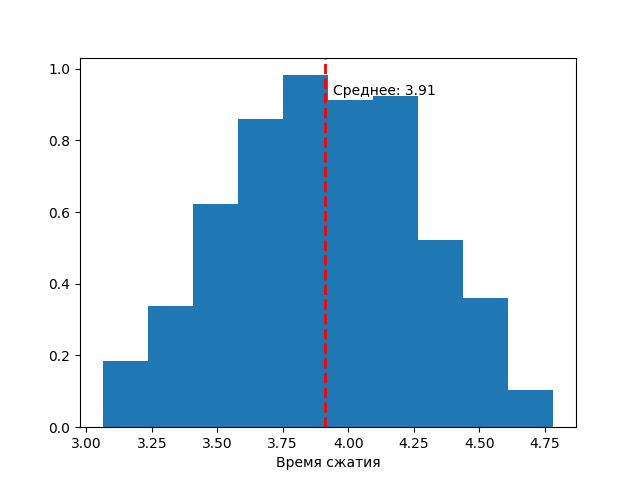
\includegraphics{images/hist-handmade-c-dev.png}
    \end{adjustbox}
    \caption{Время сжатия разработанным с нуля C-устройством.}\label{fig:hist-handmade-c-dev}
\end{figure}


\begin{figure}[!htbp]
    \centering
    \begin{adjustbox}{max totalsize={\textwidth}{\textheight}}
        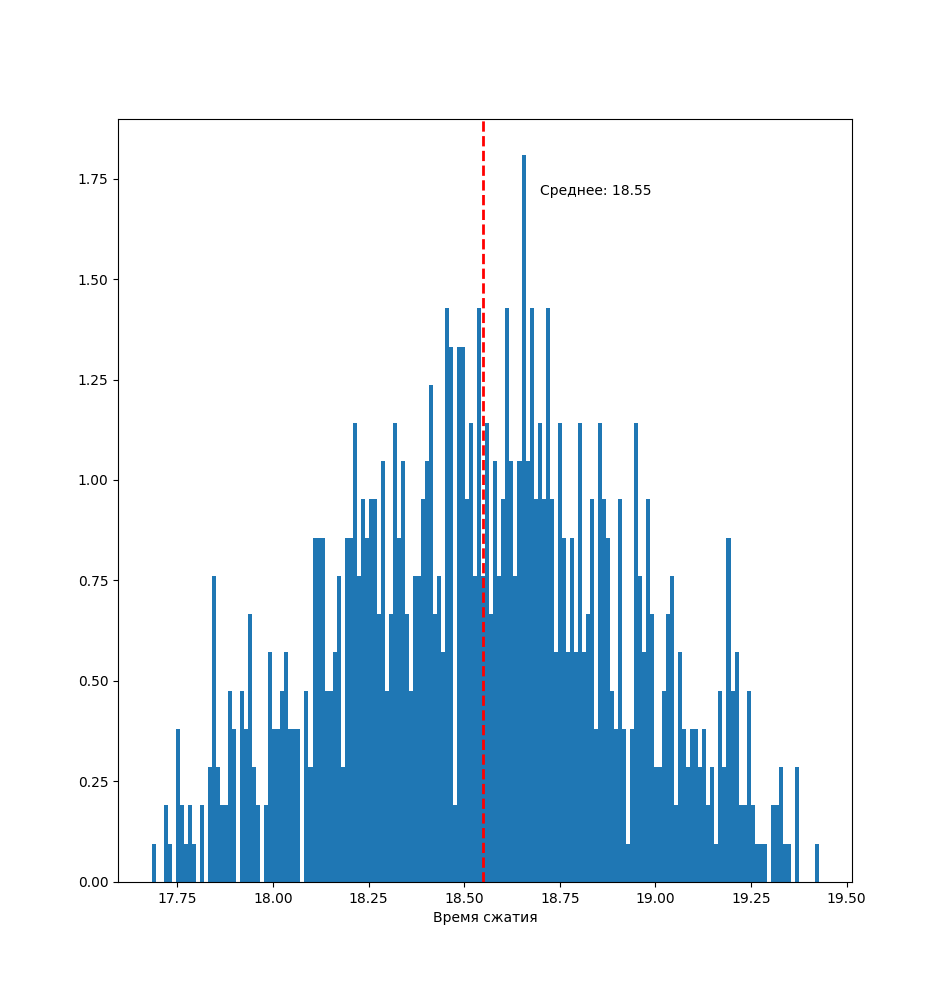
\includegraphics{images/hist-handmade-py-dev.png}
    \end{adjustbox}
    \caption{Время сжатия разработанным с нуля Python-устройством.}\label{fig:hist-handmade-py-dev}
\end{figure}


\begin{figure}[!htbp]
    \centering
    \begin{adjustbox}{max totalsize={\textwidth}{\textheight}}
        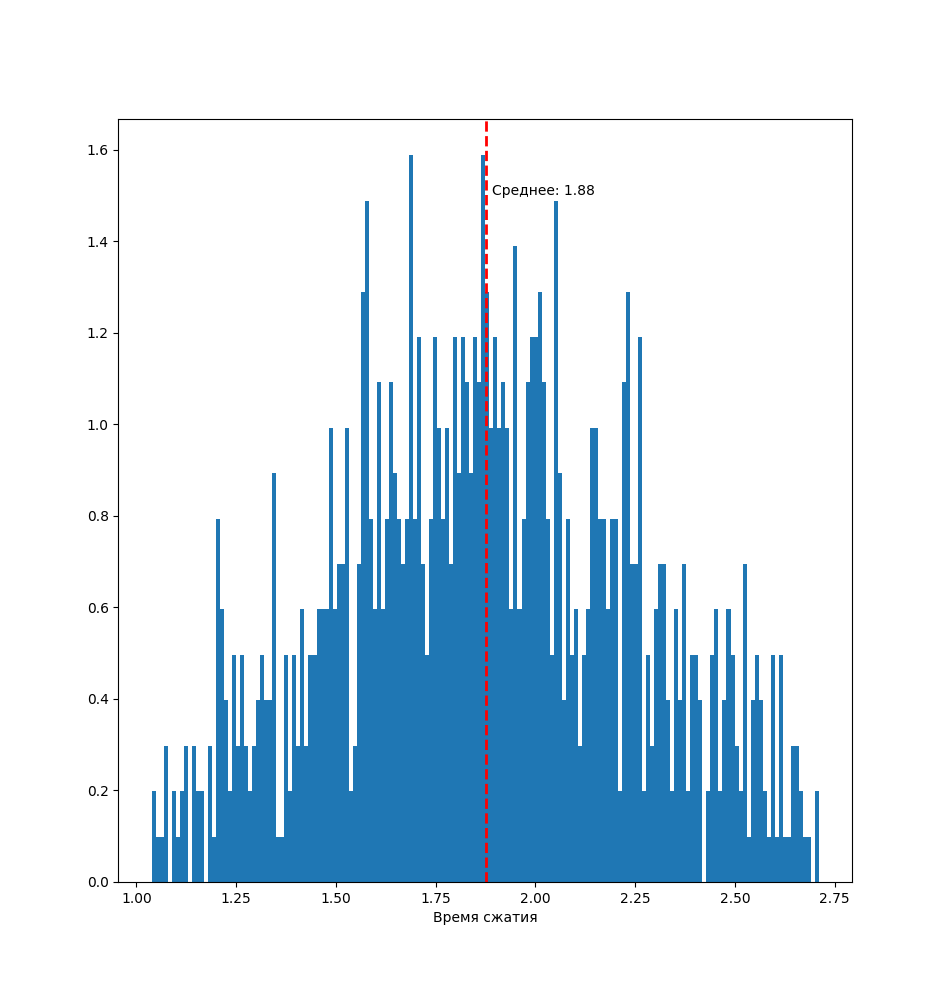
\includegraphics{images/hist-lib-c-dev.png}
    \end{adjustbox}
    \caption{Время сжатия C-устройством, использующим библиотеку.}\label{fig:hist-lib-c-dev}
\end{figure}


\begin{figure}[!htbp]
    \centering
    \begin{adjustbox}{max totalsize={\textwidth}{\textheight}}
        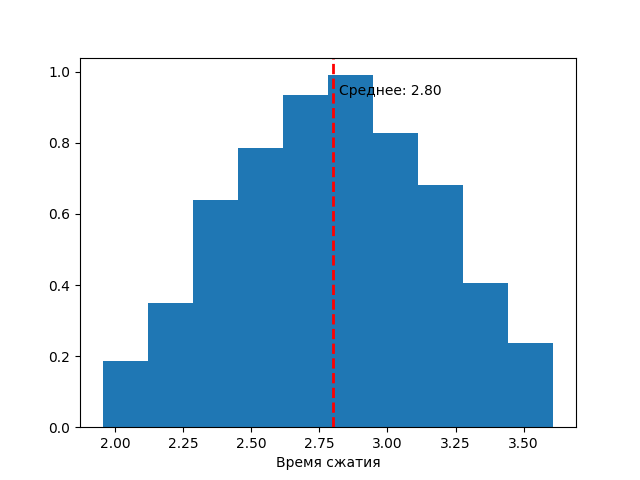
\includegraphics{images/hist-lib-py-dev.png}
    \end{adjustbox}
    \caption{Время сжатия Python-устройством, использующим библиотеку.}\label{fig:hist-lib-py-dev}
\end{figure}

\textbf{Вывод:} при создании устройства на C, очевидна разница
в скорости разработки -- имплементация устройства с нуля
требует серьезных усилий и знаий от программиста, большое количество
времени, как и возможные деструктивные ошибки связаны с управлением
памятью. Создание устройства с помощью {\mylanguage} позволяет
сократить время разработки вдвое, так как основной фокус програмиста
занят не второстепенными вещами, а реализацией алгоритма.
В то же время, использование библиотеки радикально сокращает
время разработки, но, в случае C-устройства, большое количество
времени все еще отнимает управление памятью.
Производительность, при реализации устройств без сторонних
библиотек, показывает, что Python-устройство в $4.7$ раза
медленнее аналогичного C-устройства. При использовании
библиотек, разрыв сокращается до $1.5$ раза, что связано
с накладными расходами -- библиотека обработки изображений
для Python написана как модуль, на языке C, что обеспечивает
максимальную производительность самого вычислительноемкого этапа.

\subsection{Устройство с удаленной логикой}\label{sec:ch3/sec2/sec2}

Данное устройство не реализует алгоритм сжатия JPEG картинки в себе,
а отправляет изображение внешнему обработчику,
возвращая полученное сжатое изображение в гостевую ОС.
Данная архитектура позволяет иметь, например, оптимизированный
кластер для обработки информации, к которому подключаются и с
которым общаются виртуальные устройства.

\subsubsection{Устройство, работающее через сеть}\label{sec:ch3/sec2/sec2/sec1}

В данном случае обработчиком выступает обрабатывающий узел в сети.
Реализация собственного сетевого взаимодействия не проводилась
и для него использовались сторонние библиотеки.
Данное устройство -- расширение разработанного в \ref{sec:ch3/sec2/sec1/sec1}.

\begin{longtable}{| p{5cm} | p{5cm} | p{5cm} |}
    \hline
        Метрика &
        C устройство &
        Python устройство \\
    \hline
        Суммарное Время разработки в человеко-часах &
        $45$ ($+10$) &
        $14$ ($+4$) \\
    \hline
        Время сжатия (сек.)&
        $2.341$ ($+0.47$) (рис. \ref{fig:hist-lib-c-dev}) &
        $3.533$ ($+0.75$) (рис. \ref{fig:hist-lib-c-dev}) \\
    \hline
\end{longtable}


\begin{figure}[!htbp]
    \centering
    \begin{adjustbox}{max totalsize={\textwidth}{\textheight}}
        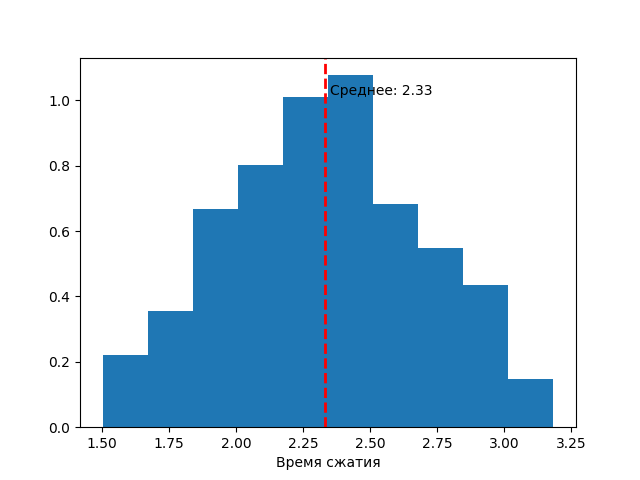
\includegraphics{images/hist-lib-c-network.png}
    \end{adjustbox}
    \caption{Время сжатия C-устройством по сети.}\label{fig:hist-lib-c-network}
\end{figure}


\begin{figure}[!htbp]
    \centering
    \begin{adjustbox}{max totalsize={\textwidth}{\textheight}}
        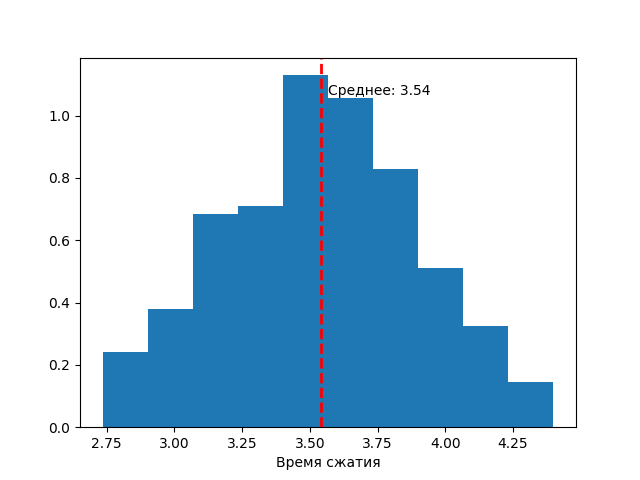
\includegraphics{images/hist-lib-py-network.png}
    \end{adjustbox}
    \caption{Время сжатия Python-устройством по сети.}\label{fig:hist-lib-py-network}
\end{figure}

\textbf{Вывод:} данный эксперимент показывает, что добавление новых возможностей,
уже реализованных сторонними библиотеками, для C-устройства занимает больше времени,
чем для Python-устройства при сопоставимой производительности.

\subsubsection{Устройство, работающее с подпроцессом}\label{sec:ch3/sec2/sec2/sec2}

В данном случае обработчиком выступает запускаемый подпроцесс сжатия
изображения.

\begin{longtable}{| p{5cm} | p{5cm} | p{5cm} |}
    \hline
    Метрика & C-устройство & Python-устройство \\
    \hline
        Время разработки в человеко-часах &
        100 часов &
        65 часов \\
    \hline
        Быстродействие &
        Быстрый метод, не требует специальных знаний о внутреннем устройстве аппаратного обеспечения &
        Взаимодействие ПО с аппаратным обеспечением ограничивается заранее записанными сценариями \\
    \hline
\end{longtable}
           % Глава 3
\chapter{Экспериментальные исследования разработанной методики и алгоритма нахождения НДВ ПО с известной моделью нарушителя}\label{ch:ch4}
           % Глава 4
\chapter*{Заключение}                       % Заголовок
\addcontentsline{toc}{chapter}{Заключение}  % Добавляем его в оглавление

%% Согласно ГОСТ Р 7.0.11-2011:
%% 5.3.3 В заключении диссертации излагают итоги выполненного исследования, рекомендации, перспективы дальнейшей разработки темы.
%% 9.2.3 В заключении автореферата диссертации излагают итоги данного исследования, рекомендации и перспективы дальнейшей разработки темы.
%% Поэтому имеет смысл сделать эту часть общей и загрузить из одного файла в автореферат и в диссертацию:

Результатом выпускной квалификационной работы стала рабочая версия
программного модуля анализа программ на языках C/C++ на недекларированные
возможности. {\ProgModule} позволил унифицировать и ускорил процесс исследования
программного обеспечения на НДВ.
Уменьшение фрагментации программ по анализу ПО на наличие НДВ позволяет
не тратить время программистов на написание анализатора под конкретный продукт,
что положительно сказывается на продуктивности всей команды разработчиков.

В рамках выпускной квалификационной работы были решены задачи:
\begin{enumerate}[label={\arabic*)}]
    \item исследование предметной области ;
    \item сравнительный анализ существующих программных решений;
    \item выбор языка и среды разработки;
    \item разработка схемы данных {\ProgModule};
    \item разработка схемы алгоритма {\ProgModule};
    \item программирование {\ProgModule};
    \item отладка и тестирование {\ProgModule};
    \item разработка документации к {\ProgModule}.
\end{enumerate}
 
В заключение автор
выражает благодарность и большую признательность научному руководителю
Кононовой Александре Игоревне за поддержку, помощь, обсуждение результатов и~научное
руководство.
      % Заключение
\include{Dissertation/references}      % Список литературы
%\include{Dissertation/lists}           % Списки таблиц и изображений (иллюстративный материал)

%%% Настройки для приложений
\appendix
% Оформление заголовков приложений ближе к ГОСТ:
\setlength{\midchapskip}{20pt}
\renewcommand*{\afterchapternum}{\par\nobreak\vskip \midchapskip}
\renewcommand\thechapter{\Asbuk{chapter}} % Чтобы приложения русскими буквами нумеровались

%\chapter{Экспериментальные данные}\label{app:A}

\begin{figure}[!htbp]
    \centering
    \begin{adjustbox}{max totalsize={0.8\textwidth}{\textheight}}
        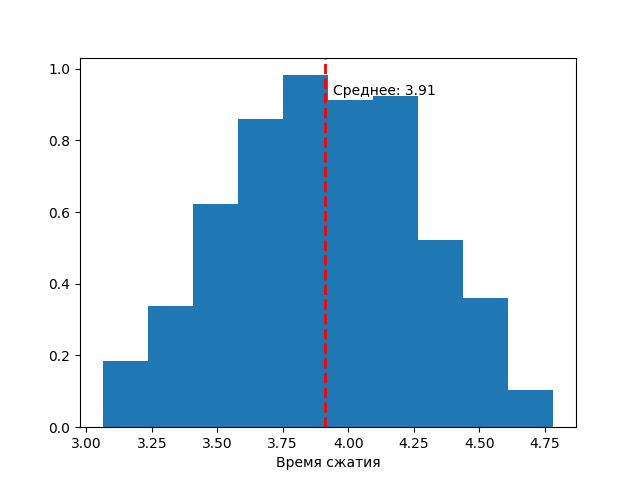
\includegraphics{images/hist-handmade-c-dev.png}
    \end{adjustbox}
    \caption{Время сжатия разработанным с нуля C-устройством.}\label{fig:hist-handmade-c-dev}
\end{figure}

{\tiny
\setlength\LTleft{-1.2cm}
    \begin{longtable}{|c|c|c|c|c|c|c|c|c|c|c|c|c|c|c|c|c|c|c|c|}%
        \caption{Время сжатия разработанным с нуля C-устройством.}\label{tbl:hist-handmade-c-dev} \\
        \hline
        № & $T$ &
        № & $T$ &
        № & $T$ &
        № & $T$ &
        № & $T$ &
        № & $T$ &
        № & $T$ &
        № & $T$ &
        № & $T$ &
        № & $T$ \\
        \hline
        \csvreader[column count=22,
                   no head,
                   table head=\hline,
                   late after line =\\\hline]{handmade-c-dev.csv}{
        1=\one, 2=\two, 3=\three, 4=\four,
        5=\five, 6=\six, 7=\seven, 8=\eight,
        9=\nine, 10=\ten, 11=\eleven, 12=\twelve,
        13=\thirteen, 14=\fourteen, 15=\fifteen, 16=\sixteen,
        17=\seventeen, 18=\eighteen, 19=\nineteen, 20=\twenty
        }
        {
            \one & \two &
            \three & \four &
            \five & \six &
            \seven & \eight &
            \nine & \ten &
            \eleven & \twelve &
            \thirteen & \fourteen &
            \fifteen & \sixteen &
            \seventeen & \eighteen &
            \nineteen & \twenty
        }
    \end{longtable}
}

\begin{figure}[!htbp]
    \centering
    \begin{adjustbox}{max totalsize={0.8\textwidth}{\textheight}}
        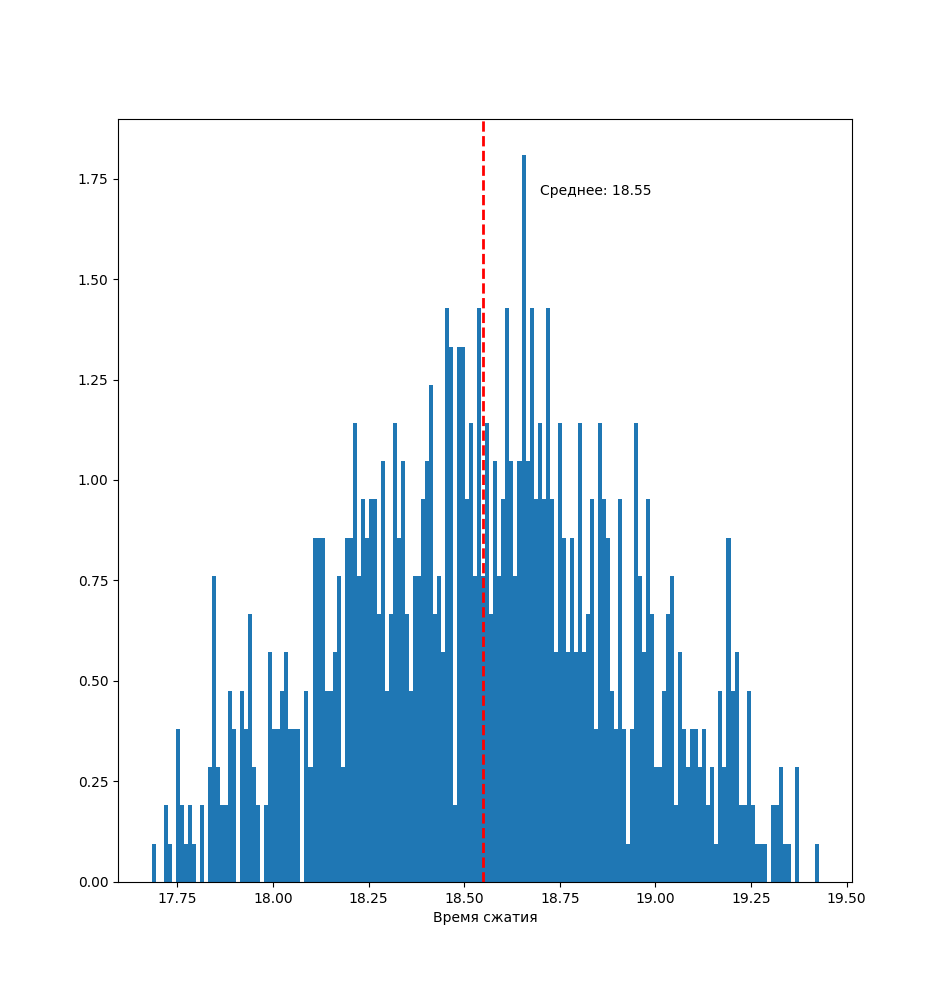
\includegraphics{images/hist-handmade-py-dev.png}
    \end{adjustbox}
    \caption{Время сжатия разработанным с нуля Python-устройством.}\label{fig:hist-handmade-py-dev}
\end{figure}

{\tiny
\setlength\LTleft{-1.5cm}
    \begin{longtable}{|c|c|c|c|c|c|c|c|c|c|c|c|c|c|c|c|c|c|c|c|}%
        \caption{Время сжатия разработанным с нуля Python-устройством.}\label{tbl:hist-handmade-py-dev} \\
        \hline
        № & $T$ &
        № & $T$ &
        № & $T$ &
        № & $T$ &
        № & $T$ &
        № & $T$ &
        № & $T$ &
        № & $T$ &
        № & $T$ &
        № & $T$ \\
        \hline
        \csvreader[column count=22,
                   no head,
                   table head=\hline,
                   late after line =\\\hline]{handmade-py-dev.csv}{
        1=\one, 2=\two, 3=\three, 4=\four,
        5=\five, 6=\six, 7=\seven, 8=\eight,
        9=\nine, 10=\ten, 11=\eleven, 12=\twelve,
        13=\thirteen, 14=\fourteen, 15=\fifteen, 16=\sixteen,
        17=\seventeen, 18=\eighteen, 19=\nineteen, 20=\twenty
        }
        {
            \one & \two &
            \three & \four &
            \five & \six &
            \seven & \eight &
            \nine & \ten &
            \eleven & \twelve &
            \thirteen & \fourteen &
            \fifteen & \sixteen &
            \seventeen & \eighteen &
            \nineteen & \twenty
        }
    \end{longtable}
}


\begin{figure}[!htbp]
    \centering
    \begin{adjustbox}{max totalsize={0.8\textwidth}{\textheight}}
        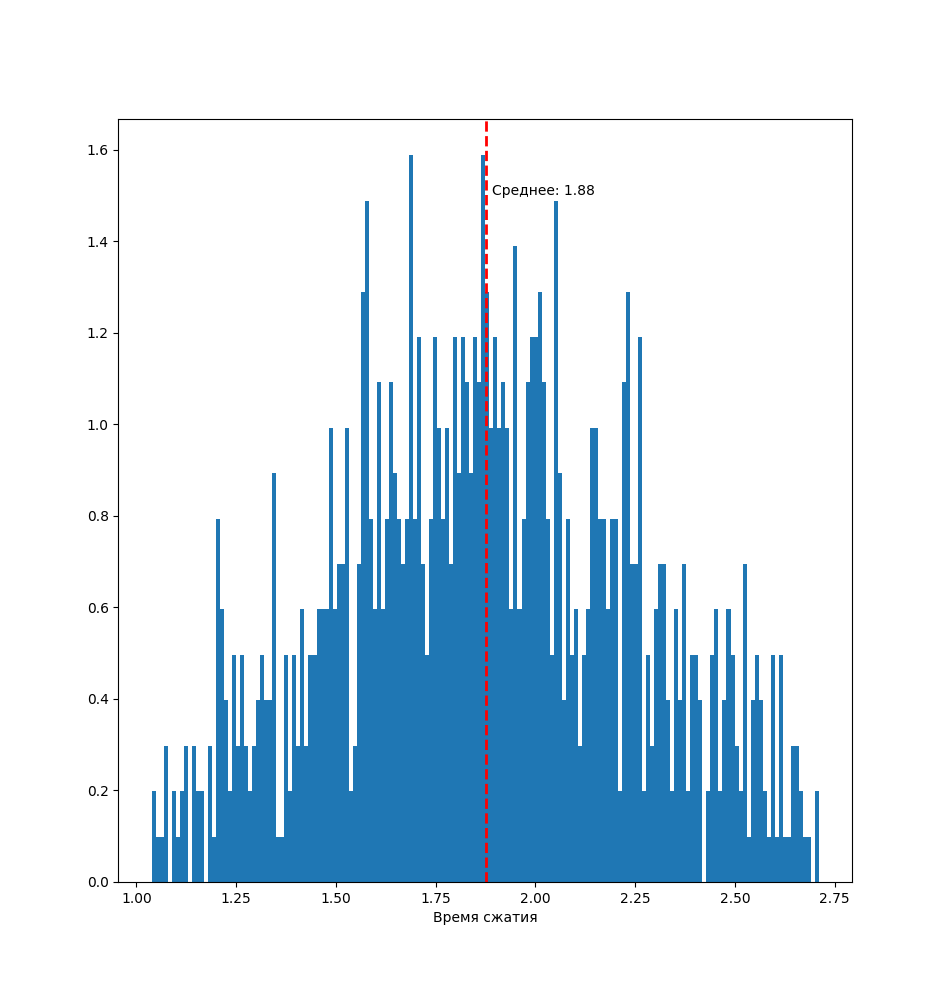
\includegraphics{images/hist-lib-c-dev.png}
    \end{adjustbox}
    \caption{Время сжатия C-устройством, использующим библиотеку сжатия.}\label{fig:hist-lib-c-dev}
\end{figure}

{\tiny
\setlength\LTleft{-1.2cm}
    \begin{longtable}{|c|c|c|c|c|c|c|c|c|c|c|c|c|c|c|c|c|c|c|c|}%
        \caption{Время сжатия C-устройством, использующим библиотеку сжатия.}\label{tbl:hist-lib-c-dev} \\
        \hline
        № & $T$ &
        № & $T$ &
        № & $T$ &
        № & $T$ &
        № & $T$ &
        № & $T$ &
        № & $T$ &
        № & $T$ &
        № & $T$ &
        № & $T$ \\
        \hline
        \csvreader[column count=22,
                   no head,
                   table head=\hline,
                   late after line =\\\hline]{lib-c-dev.csv}{
        1=\one, 2=\two, 3=\three, 4=\four,
        5=\five, 6=\six, 7=\seven, 8=\eight,
        9=\nine, 10=\ten, 11=\eleven, 12=\twelve,
        13=\thirteen, 14=\fourteen, 15=\fifteen, 16=\sixteen,
        17=\seventeen, 18=\eighteen, 19=\nineteen, 20=\twenty
        }
        {
            \one & \two &
            \three & \four &
            \five & \six &
            \seven & \eight &
            \nine & \ten &
            \eleven & \twelve &
            \thirteen & \fourteen &
            \fifteen & \sixteen &
            \seventeen & \eighteen &
            \nineteen & \twenty
        }
    \end{longtable}
}

\begin{figure}[!htbp]
    \centering
    \begin{adjustbox}{max totalsize={0.8\textwidth}{\textheight}}
        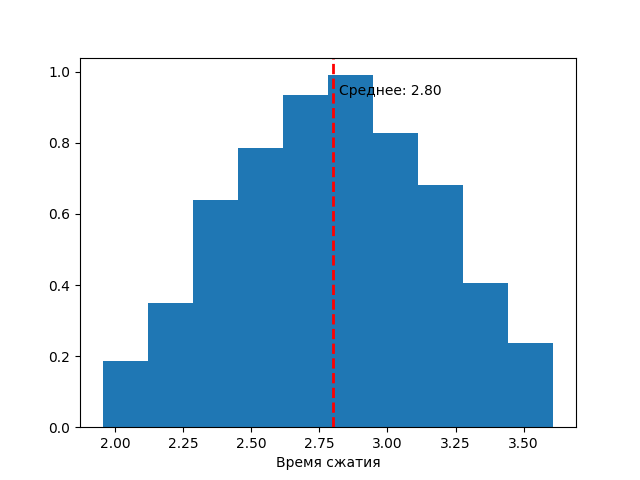
\includegraphics{images/hist-lib-py-dev.png}
    \end{adjustbox}
    \caption{Время сжатия Python-устройством, использующим библиотеку сжатия.}\label{fig:hist-lib-py-dev}
\end{figure}

{\tiny
\setlength\LTleft{-1.5cm}
    \begin{longtable}{|c|c|c|c|c|c|c|c|c|c|c|c|c|c|c|c|c|c|c|c|}%
        \caption{Время сжатия Python-устройством, использующим библиотеку сжатия.}\label{tbl:hist-lib-py-dev} \\
        \hline
        № & $T$ &
        № & $T$ &
        № & $T$ &
        № & $T$ &
        № & $T$ &
        № & $T$ &
        № & $T$ &
        № & $T$ &
        № & $T$ &
        № & $T$ \\
        \hline
        \csvreader[column count=22,
                   no head,
                   table head=\hline,
                   late after line =\\\hline]{lib-py-dev.csv}{
        1=\one, 2=\two, 3=\three, 4=\four,
        5=\five, 6=\six, 7=\seven, 8=\eight,
        9=\nine, 10=\ten, 11=\eleven, 12=\twelve,
        13=\thirteen, 14=\fourteen, 15=\fifteen, 16=\sixteen,
        17=\seventeen, 18=\eighteen, 19=\nineteen, 20=\twenty
        }
        {
            \one & \two &
            \three & \four &
            \five & \six &
            \seven & \eight &
            \nine & \ten &
            \eleven & \twelve &
            \thirteen & \fourteen &
            \fifteen & \sixteen &
            \seventeen & \eighteen &
            \nineteen & \twenty
        }
    \end{longtable}
}


\begin{figure}[!htbp]
    \centering
    \begin{adjustbox}{max totalsize={0.8\textwidth}{\textheight}}
        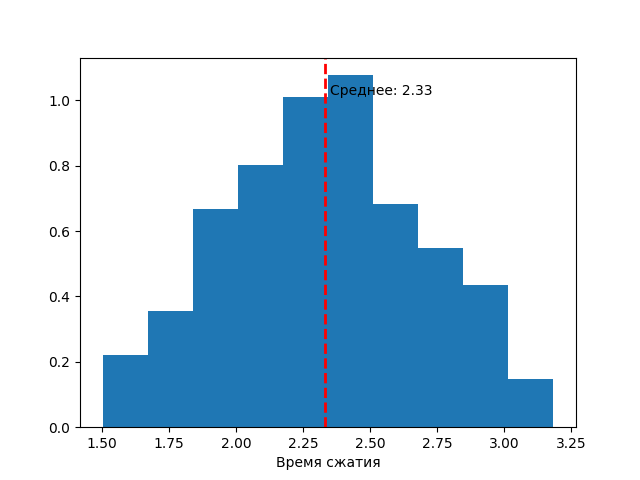
\includegraphics{images/hist-lib-c-network.png}
    \end{adjustbox}
    \caption{Время сжатия C-устройством по сети.}\label{fig:hist-lib-c-network}
\end{figure}


\begin{figure}[!htbp]
    \centering
    \begin{adjustbox}{max totalsize={0.8\textwidth}{\textheight}}
        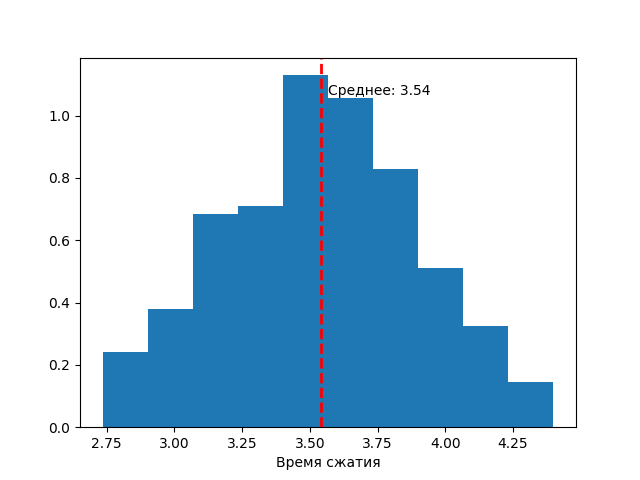
\includegraphics{images/hist-lib-py-network.png}
    \end{adjustbox}
    \caption{Время сжатия Python-устройством по сети.}\label{fig:hist-lib-py-network}
\end{figure}

\begin{figure}[!htbp]
    \centering
    \begin{adjustbox}{max totalsize={0.8\textwidth}{\textheight}}
        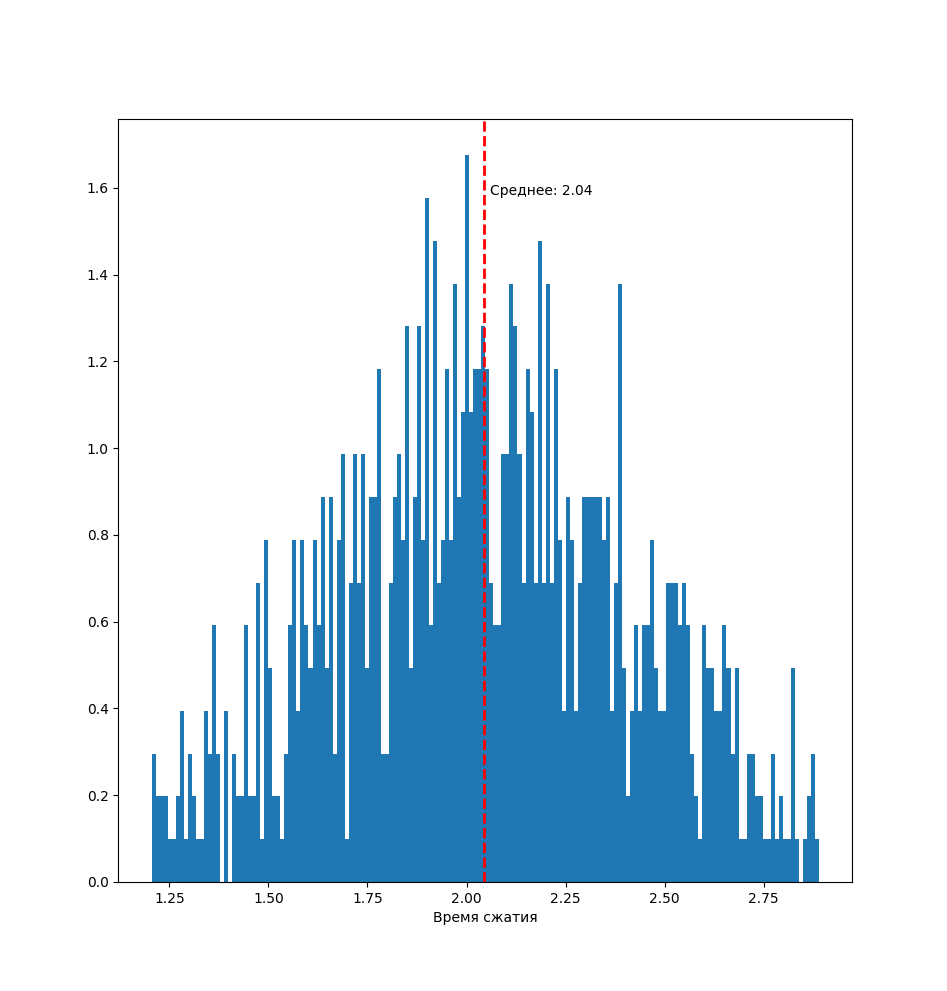
\includegraphics{images/hist-exec-c-dev.png}
    \end{adjustbox}
    \caption{Время сжатия C-устройством через подпроцесс.}\label{fig:hist-exec-c-dev}
\end{figure}

\begin{figure}[!htbp]
    \centering
    \begin{adjustbox}{max totalsize={0.8\textwidth}{\textheight}}
        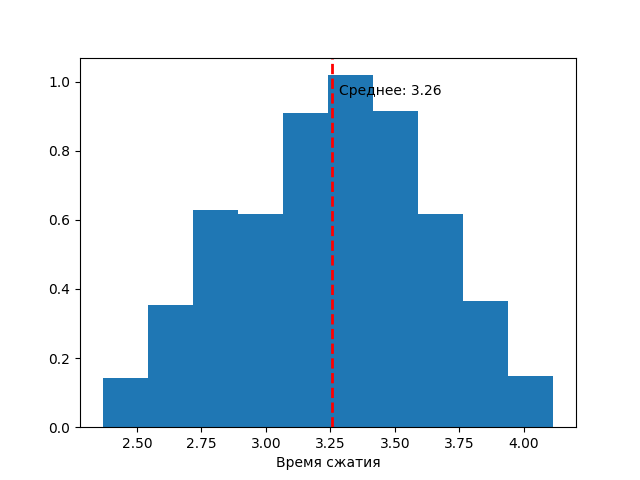
\includegraphics{images/hist-exec-py-dev.png}
    \end{adjustbox}
    \caption{Время сжатия Python-устройством через подпроцесс.}\label{fig:hist-exec-py-dev}
\end{figure}



\chapter{Программный код}\label{app:B}

Proof Of Concept реализация {\mylanguage}, \cref{lst:core.template.c,lst:main.py,lst:schema_parser.py}.

\begin{lstlisting}[language={C},basicstyle=\tiny,stepnumber=1,caption={Шаблон устройства},label={lst:core.template.c}]
#include "qemu/osdep.h"
#include "qapi/error.h"
#include "qom/object.h"
/*[[[cog
    import json as j
    import main as m

    with open(m.DEV_SCHEMA_FILE, 'r') as sf:
        SCHEMA = j.load(sf)

    device_header = SCHEMA["parent"]["header"]
    cog.outl(f'#include "{device_header}"')
   ]]]*/
/*[[[end]]]*/
#include "exec/address-spaces.h"
#include "hw/qdev-properties-system.h"

#include <Python.h>

#define IF_NULL_GOTO_ERR(VAR, BODY) \
    BODY; \
    if (!VAR){ \
        goto err; \
    }

#define PY_COMPILE_AND_GET_FUNC(FUNC_NAME, PY_CODE, PY_COMPILED, PY_MODULE, PY_FUNC) \
    if (!PY_COMPILED){ \
        IF_NULL_GOTO_ERR(PY_COMPILED, \
                         PY_COMPILED = Py_CompileString(PY_CODE, FUNC_NAME ".py", Py_single_input)) \
    } \
    IF_NULL_GOTO_ERR(PY_MODULE, \
                     PY_MODULE = PyImport_ExecCodeModule(FUNC_NAME "module", PY_COMPILED)) \
    IF_NULL_GOTO_ERR(PY_FUNC, \
                     PY_FUNC = PyObject_GetAttrString(PY_MODULE, FUNC_NAME))


typedef struct {
    char *name;
    size_t size;
} DeviceFieldMetaInfo;


/*[[[cog
    #
    # generating device class
    #

    import json as j
    import main as m
    from textwrap import indent, dedent
    INDENT = lambda s: indent(s, ' '*4)

    with open(m.DEV_SCHEMA_FILE, 'r') as sf:
        SCHEMA = j.load(sf)


    device_class    = m.get_device_class_name(SCHEMA, full = True)
    device_instance = m.get_device_class_name(SCHEMA)
    device_parent   = SCHEMA["parent"]["name"]


    cog.outl("typedef struct {")
    cog.outl(INDENT(f"{device_parent}Device parent_obj;"))
    cog.outl(f"}} {device_class};")
    cog.outl()
    cog.outl(f"typedef struct __attribute__((packed)) {{")
    for fname, ftype in m.get_nested_schema(SCHEMA, "device").items():
        cog.outl(INDENT(f"{ftype} {fname};"))
    cog.outl(f"}} {device_instance};")

    cog.outl()
    cog.outl()
    cog.outl(f"DeviceFieldMetaInfo device_fields[] = {{")
    for fname, ftype in m.get_nested_schema(SCHEMA, "device").items():
        cog.outl(INDENT(f'{{ "{fname}", sizeof({ftype}) }},'))
    cog.outl(INDENT('};'))
  ]]]*/
/*[[[end]]]*/

#define DEVICE_FIELDS_COUNT sizeof(device_fields)/sizeof(device_fields[0])

static PyObject* create_dict_for_class_fields(){
    PyObject* p_field_dicts[DEVICE_FIELDS_COUNT];
    PyObject *p_meta_info_aggregation = PyDict_New();
    for(int i = 0; i < DEVICE_FIELDS_COUNT; i++){
        int err = PyDict_Merge(p_meta_info_aggregation,
                               Py_BuildValue("{s:i}",
                                             device_fields[i].name,
                                             device_fields[i].size),
                               1);
        if(err){
            PyErr_Print();
            abort();
        }
    }
    return p_meta_info_aggregation;
}

PyObject *DictWithClassFields;

/*[[[cog
    #
    # generating device type
    #

    import json as j
    import main as m

    with open(m.DEV_SCHEMA_FILE, 'r') as sf:
        SCHEMA = j.load(sf)

    device_instance    = m.get_device_class_name(SCHEMA)
    device_name        = SCHEMA["name"]
    device_parent_type = SCHEMA["parent"]["type"]
    device_interface   = SCHEMA["parent"]["interface"]
    device_qtype       = SCHEMA["name"].upper()

    cog.outl(f'#define TYPE_{device_qtype} "{device_name}"')
    cog.outl(f"""OBJECT_DEFINE_TYPE_WITH_INTERFACES({device_instance},
                                       {device_name},
                                       {device_qtype},
                                       {device_parent_type}_DEVICE,
                                       {{ INTERFACE_{device_interface} }},
                                       {{ NULL }})""")
  ]]]*/
/*[[[end]]]*/

/*[[[cog
    #
    # generating function prototypes
    #

    import json as j
    import main as m
    from textwrap import indent, dedent
    INDENT = lambda s: indent(s, ' '*4)

    with open(m.DEV_SCHEMA_FILE, 'r') as sf:
        SCHEMA = j.load(sf)

    class_methods = SCHEMA["class"]["schema"]["methods"]
    class_init = m.create_device_method_proto(SCHEMA, "void", "class_init", "ObjectClass *oc, void *data")
    cog.outl(f"{class_init};")

    for method in class_methods:
        cog.outl(f'{m.create_device_method_proto(SCHEMA, method["c_ret"], method["c_name"], method["c_args"])};')
  ]]]*/
/*[[[end]]]*/

/*[[[cog
    #
    # generating device properties
    #

    import json as j
    import main as m
    from textwrap import indent, dedent
    INDENT = lambda s: indent(s, ' '*4)

    with open(m.DEV_SCHEMA_FILE, 'r') as sf:
        SCHEMA = j.load(sf)

    device_name = SCHEMA['name']

    cog.outl(f"static Property {device_name}_properties[] = {{")
    for p in m.get_nested_schema(SCHEMA, 'properties'):
        ptype         = p["type"].upper()
        pname         = f"\"{p['name']}\""
        pfield        = p["field"]
        dev_name      = m.get_device_class_name(SCHEMA)
        default_value = ''

        if "default_value" in p:
            default_value = ', ' + str(p["default_value"])

        cog.outl(INDENT(f"DEFINE_PROP_{ptype}({pname}, {dev_name}, {pfield}{default_value}),"))
    cog.outl(INDENT("DEFINE_PROP_END_OF_LIST()"))
    cog.outl("};")
  ]]]*/
/*[[[end]]]*/

/*[[[cog
    #
    # generating device MemoryRegionOps
    #

    import json as j
    import main as m
    from textwrap import indent, dedent
    INDENT = lambda s: indent(s, ' '*4)

    with open(m.DEV_SCHEMA_FILE, 'r') as sf:
        SCHEMA = j.load(sf)

    device_name = SCHEMA['name']

    for k,v in m.get_nested_schema(SCHEMA, "device").items():
        if v == "MemoryRegionOps":
            cog.outl(f"static const MemoryRegionOps {device_name}_mem_ops = {{")
            for mem_k, mem_v in SCHEMA["device"]["schema"][k].items():
                cog.outl(INDENT(f".{mem_k} = {mem_v},"))

            cog.outl(INDENT(f".read = {m.get_method_name(SCHEMA, 'read')},"))
            cog.outl(INDENT(f".write = {m.get_method_name(SCHEMA, 'write')},"))

            cog.outl("};")
  ]]]*/
/*[[[end]]]*/

/*[[[cog
    #
    # generating device and instance methods
    #

    import re
    import json as j
    import main as m

    from textwrap import indent, dedent
    INDENT = lambda s: indent(s, ' '*4)
    ALIGN_INDENT_BY = lambda s: ' ' * len(s)

    with open(m.DEV_SCHEMA_FILE, 'r') as sf:
        SCHEMA = j.load(sf)


    device_name      = SCHEMA["name"]
    class_init_proto = m.create_device_method_proto(SCHEMA, "void", "class_init", "ObjectClass *oc, void *data")

    cog.outl(f"{class_init_proto}{{")

    class_field_init = SCHEMA["class"]["schema"]["init"]["class_field_init"]

    if not any(filter(lambda cast: cast["dev_cast"]["type"] == "DeviceClass",
                      class_field_init)):
        default_dev_cast = {"dev_cast": {"type" : "DeviceClass", "cast": "DEVICE_CLASS"}}
        class_field_init = [default_dev_cast] + class_field_init

    for entry in class_field_init:
        cog.outl()
        dev_cast   = entry["dev_cast"]
        cast_type  = dev_cast['type']
        cast_macro = dev_cast['cast']

        cog.outl(INDENT(f"{cast_type} *{cast_type}_ptr = {cast_macro}(oc);"))

        for k,v in entry.items():
            if k == "dev_cast":
                continue
            cog.outl(INDENT(f"{cast_type}_ptr->{k} = {v};"))


    cog.outl(INDENT(f"device_class_set_props(DeviceClass_ptr, {device_name}_properties);"))

    cog.outl()
    cog.outl(INDENT(f'Py_SetProgramName("{device_name}");'))
    cog.outl(INDENT(f'Py_Initialize();'))
    cog.outl(INDENT(f'DictWithClassFields = create_dict_for_class_fields();'))
    cog.outl("}")
    cog.outl()
    cog.outl()

    for method in class_methods:
        method_proto = m.create_device_method_proto(SCHEMA, method["c_ret"], method["c_name"], method["c_args"])
        argc = method["c_args"].count(',') + 1
        arguments = [s.strip() for s in method["c_args"].split(',')]
        casts = [s.strip() for s in method["c_to_py_cast"].split(',')]

        argument_type_val = [arg.split() for arg in arguments]
        arguments_and_cast = list(zip(argument_type_val, casts))

        if len(argument_type_val) != len(arguments_and_cast):
            cog.error(f"{argument_type_val} and {casts} length mismatch!")

        cog.outl(f"{method_proto}{{")

        pass_args_to_python = ''
        memoryview_vars = []
        for i, (arg, cast) in enumerate(arguments_and_cast):
            is_pointer = '*' in arg[0] + arg[1]
            arg_val = arg[1].replace('*', '')
            if is_pointer:
                arg_val_as_buf = arg_val
            else:
                arg_val_as_buf= '&' + arg_val

            if method["c_name"] == "realize" and \
               "MemoryRegionOps" in m.get_nested_schema(SCHEMA, "device").values():
                device_fields = m.get_nested_schema(SCHEMA, "device")
                reverse_device_fields = dict(zip(device_fields.values(), device_fields.keys()))
                mem_io_field = reverse_device_fields["MemoryRegionOps"]
                cog.outl(INDENT(f"memory_region_init_io(&(({cast}*){arg_val_as_buf})->{mem_io_field},"))
                cog.outl(INDENT(f"                      OBJECT({arg_val_as_buf}),"))
                cog.outl(INDENT(f"                      &{device_name}_mem_ops,"))
                cog.outl(INDENT(f"                      {arg_val_as_buf},"))
                cog.outl(INDENT(f'                      "{device_name}-mmio",'))
                cog.outl(INDENT(f"                      1);"))

            memoryview_vars.append(f"p_mem_view_{arg_val}")
            pass_args_to_python += INDENT(INDENT(dedent(f"""
                                                 PyObject *p_mem_view_{arg_val} = PyMemoryView_FromMemory((char*){arg_val_as_buf},
                                                                                                 {ALIGN_INDENT_BY(arg_val)}sizeof({cast}),
                                                                                                 {ALIGN_INDENT_BY(arg_val)}PyBUF_WRITE);
                                                 if (!p_mem_view_{arg_val}){{
                                                     goto err;
                                                 }}
                                                 PyTuple_SetItem(p_func_args, {i}, p_mem_view_{arg_val});
                                                 """)))

            memoryview_vars_free = INDENT('\n'.join([f'Py_XDECREF({mv});' for mv in memoryview_vars]))
            py_return_code = ''
            py_return_val_name = ''
            if method["c_ret"] != "void":
                py_return_val_name = 'py_out'
                py_return_code = INDENT(dedent(f"""
                                        char *py_out_buf;
                                        {method["c_ret"]} {py_return_val_name};
                                        int ok = PyArg_ParseTuple(p_ret, "S", &py_out_buf);
                                        {py_return_val_name} = *({method["c_ret"]}*)py_out_buf;
                                        """))

        pass_args_to_python += INDENT(INDENT(f"PyTuple_SetItem(p_func_args, {argc}, DictWithClassFields);\n"))
        c_function_body = m.get_python_c_api_wrap(SCHEMA,
                                                  'class',
                                                  method["py_name"],
                                                  argc + 1,
                                                  pass_args_to_python,
                                                  return_val=py_return_val_name)
        if method["c_name"] == "finalize":
            err_handling_code = "if(Py_FinalizeEx()){\n" \
                                + INDENT(INDENT("PyErr_Print();\n")) \
                                + INDENT(INDENT("abort();\n")) \
                                + INDENT("}\n")
            c_function_body = re.sub("//.*?\n",
                                     err_handling_code + memoryview_vars_free + '\n',
                                     c_function_body)
        else:
            c_function_body = re.sub("\s+//.*?\n", f"\n{py_return_code}\n{memoryview_vars_free}\n", c_function_body, count=1)
            c_function_body = re.sub("\s+//.*?\n", f"\n{memoryview_vars_free}\n", c_function_body, count=1)
        c_function_body = '\n'.join(filter(lambda l: not re.match("\s+$", l), c_function_body.splitlines()))
        cog.outl(c_function_body)

        cog.outl("}")
        cog.outl()
        cog.outl()
  ]]]*/
/*[[[end]]]*/
\end{lstlisting}


\begin{lstlisting}[language={Python},basicstyle=\tiny,stepnumber=1,caption={Вспомогательные методы кодогенерации},label={lst:main.py}]
import os
import sys
import json
import inspect
import importlib.util
import subprocess as subp

from pathlib import Path
from textwrap import dedent

import schema_parser as sp


def get_nested_schema(schema: dict, key: str):
    return schema[key]['schema'][key]


def get_device_class_name(schema: dict, full=False):
    base_class_name = schema["name"].replace('_', ' ').title().replace(' ', '')
    if full:
        return base_class_name + "Class"
    return base_class_name


def get_function_text_from(sub_schema: dict, method_name: str):
    spec = importlib.util.spec_from_file_location("py_code", sub_schema["code"])
    py_code = importlib.util.module_from_spec(spec)
    spec.loader.exec_module(py_code)
    return inspect.getsource(getattr(py_code, method_name)).split('\n')


def get_python_c_api_wrap(schema: dict,
                          _from: str,
                          func_name: str,
                          tuple_size: int,
                          code_for_insert: str,
                          return_val: str = ''):
    c_char_source = [l + '\\n' for l in get_function_text_from(schema[_from], func_name)]

    py_code = f"static char *py_code = "
    py_code_start = len(py_code) + 8

    py_code += f'"{c_char_source[0]}"\n'
    for line in c_char_source[1:-1]:
        py_code += py_code_start*' ' + f'"{line}"\n'
    py_code += py_code_start*' ' + f'"{c_char_source[-1]}";'

    check_code = """if (!{what}){{
            goto err;
        }}"""

    return dedent(f"""
        {py_code}
        static PyObject *p_compiled_code = NULL;
        PyObject *p_module = NULL,
                 *p_func = NULL,
                 *p_func_args = NULL,
                 *p_ret = NULL;

        PY_COMPILE_AND_GET_FUNC("{func_name}",
                                py_code,
                                p_compiled_code,
                                p_module,
                                p_func);

        p_func_args = PyTuple_New({tuple_size});
        {check_code.format(what='p_func_args')}
        {code_for_insert}
        p_ret = PyObject_CallObject(p_func, p_func_args);
        {check_code.format(what='p_ret')}

        // for post creation code insert
        Py_XDECREF(p_module);
        Py_XDECREF(p_func);
        Py_XDECREF(p_func_args);
        Py_XDECREF(p_ret);
        return {return_val};

    err:
        PyErr_Print();
        // for post creation code insert
        Py_XDECREF(p_module);
        Py_XDECREF(p_func);
        Py_XDECREF(p_func_args);
        Py_XDECREF(p_ret);
        abort();
        """)


def get_method_name(schema: dict,
                    method_name: str):
    return f"{schema['name']}_{method_name}"


def create_device_method_proto(schema: dict,
                               ret_type: str,
                               method_name: str,
                               args: str,
                               static=True):
    method_proto = f"{ret_type} {get_method_name(schema, method_name)}({args})"
    if static:
        return f"static {method_proto}"
    return method_proto


DEV_SCHEMA_FILE = 'concrete_dev_schema.json'

if __name__ == '__main__':
    ENV = os.environ.copy()
    ENV["PYTHONPATH"] = Path('.').absolute()
    SCHEMA = sp.load_schema(sys.argv[1])

    with open(DEV_SCHEMA_FILE, 'w') as cds:
        json.dump(SCHEMA, cds, indent=2)


    subp.run(['cog', '-d', '-o', SCHEMA["name"] + '.c', sys.argv[2]],
             env=ENV)
\end{lstlisting}


\begin{lstlisting}[language={Python},basicstyle=\tiny,stepnumber=1,caption={Парсер схемы},label={lst:schema_parser.py}]
import json
import typing as t

from pathlib import Path


def load_schema(filename: str):
    schema_path = Path(filename)

    def get_load_path(path: Path):
        return path if path.is_absolute() else schema_path.parent / path

    def load_into_schema(schema_slice: dict,
                         key: str,
                         path: Path,
                         as_json=True):
        with open(path, 'r') as f:
            if as_json:
                schema_slice[key] = json.load(f)
            else:
                schema_slice[key] = f.read()


    with open(schema_path, 'r') as f:
        init_schema = json.load(f)
        for k in filter(lambda k: type(init_schema[k]) == dict and \
                                  'schema' in init_schema[k] and \
                                  'code' in init_schema[k], init_schema):
            subschema_path = get_load_path(Path(init_schema[k]['schema']))
            subschema_code = get_load_path(Path(init_schema[k]['code']))
            load_into_schema(init_schema[k], 'schema', subschema_path)
            init_schema[k]['code'] = str(subschema_code)

    return init_schema
\end{lstlisting}
        % Приложения

\end{document}
